\documentclass{book}

\usepackage[paperheight=11in,paperwidth=8.5in]{geometry}

\usepackage{graphicx, subfigure}

\setlength{\oddsidemargin}{0pt}  
\setlength{\evensidemargin}{0pt}  



\pdfpxdimen=1in

\divide\pdfpxdimen by 300

\begin{document}
\title{GENEALOGY OF THE CRANE FAMILY VOLUME I.}
\author{ELLEREY BICKNELL CRANE}

\maketitle

\begin{figure}[t]
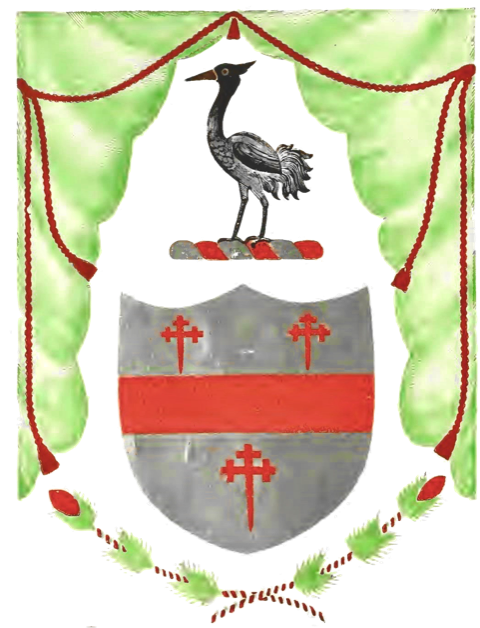
\includegraphics{../mouthOfHorse/crest1.png}
\centering
\end{figure}

\tableofcontents

\chapter{Introductory Material}

\section{Editor's Notes}

This is a \LaTeX $\:$ version of "Ellerey Crane's GENEOLOGY OF THE CRANE FAMILY, VOLUME 1." first published in 1895. This project can be viewed on github at \texttt{https://github.com/NolanC33/geneBook}

\subsection{Dedication}

For my father - happy belated birthday!

\subsection{Motivation}

I endeavored to create this project for the following reasons: 

\begin{enumerate}
\item I couldn't find a good place to buy a hard copy version of this book
\item There is a .txt version of this book found at \texttt{https://archive.org/details/genealogyofcrane02cran}
\item Creating a "modern" version of the book would be a fun project
\item I can put the end product online for anyone to see. 
\end{enumerate}

\subsection{Process}

This whole project is possible because somebody turned the actual book into a \texttt{.pdf} file, and then Optical Character Recognition (OCR) was applied to that \texttt{.pdf} to create a \texttt{.txt} file, which was the "input" to this process. All the errors in translation are the result of incorrect OCR, and there are plenty, which is unfortunate but can't be helped. 

The file \texttt{MakePretty.py} contains most of the details as to how this project was completed, which can be found on the project GitHub. What was ultimately being done here was converting the \texttt{.txt} file (the result of the OCR) to this \texttt{.tex} file, which can be compiled into \texttt{.pdf}.  Here is a rough overview of what was done: 

\begin{enumerate}
\item Removed all the unprintable characters. 
\item All the characters that are \LaTeX $\:$ control sequences were escaped.
\item Chapters and sections were added 
\item Manual revision
\begin{enumerate}
\item Fixed all the titles and sections
\item Added in the pictures
\end{enumerate}
\end{enumerate}

\subsection{Last Notes}

As stated before, there are a lot of spelling mistakes, unfortunately. The original index was also removed because the OCR did not interpret it in a way that makes sense as an index. 

The pages numbers referred to in the document reference the OLD page numbers, not the page numbers that you see in this document. 

\section{Preface}

THE observance of the Centennial anniversary of the Birth of 
our Nation as a Republic in 1876, drew the attention of every 
patriotic citizen to the charming picture to be seen by a careful 
retrospective view of the past history of the growth and develop- 
ment of our government and Nation. It also fanned into a tlame 
of activity the then smoldering desire among American people 
to know something of their ancestry. The brilliant achievements 
of men throughout the various walks of life became emphasized 
through the means and influence of that Centennial anniversary, 
inquiries regarding the earl\}' founders of New England l)egan 
rapidly to multiply, and during the past fifteen years family 
histories have appeared in comparatively rapid succession. 

It was about the year 1876 that tlie writer became interested 
in gathering materials for a history of the Ckaxe Family, and 
on Wednesday, the -Sth of September, 1880, a company of descendants from the early emigrants to this coiuitry who bore that [)atro- 
nymic, met at the Elliott House in New Haven, Conn., to con- 
sider the advisability of publishing a family history. It was an 
exceedingly enjoyal)le occasion, the expression on every hand was 
decidedly in favor of completing the undertaking. After the 
report of progress in collecting materials for the work, and the 
attempt to ascertain the location from whence our emigrants came 
to this country had been made ])y the writer, an organization for 
business was effected by the choice of Robert Crane, j\\1.1)., of 
New Haven, Chairman, and Mr. William R. Crane of Hartford, 
Secretary. A motion to form an association for carrying for- 
ward the work passed unanimously, and a committee was at once 
selected to rei)ort on a permanent organization. After full discussion had been given to the delectable dinner prepared by land- 
lord Samuel H. Crane, the party again entered the parlors to 



listen to the following report from their committee : ' ' Name of 
the Society to be The Crane Genealogical Association ; Presi- 
dent, Zenas M. Crane, Dalton, Mass. ; Vice-Presidents, Gen. 
NiROM M. Crane, Horn ells ville, N. Y., Phineas M. Crane, Jr., 
p]ast Boston, Mass. ; Secretary and Treasurer, Ellery B. 
Crane, Worcester, Mass. Executive Committee, Dr. Sajhel 
L. G. Crane, Hartford, Conn., James E. Crane, New York 
City, Robert Crane, M.D., New Haven, Conn., Rev. Elias N. 
Crane, Norfolk, Va., Augustus S. Crane, Elizabeth town, N. 
J., Albert Crane, Esq., New York City. President of the 
Association to be ex-officio member of the Committee." 

This report was accepted and its recommendations adopted. 
It was further voted that the P'xecutive Committee be empowered 
to take all necessary steps to perfect the organization and arrange 
for a general meeting of the family to be held in the future at 
such time and place as they might determine. An interesting 
sketch of Col. John Crane of Revolutionary fame, descendant 
of Henry of Dorchester, Mass., prepared by Mr. George Hay- 
ward Allen of Boston, was read by Albert Crane, Esq., of New 
York City, the author not being able to be present. It was then 
voted to open a subscription list for the piu'pose of raising funds 
with which to defray the expense of collecting genealogical data 
and for locating, if possible, the home of our emigrants on the 
otiier side of the Atlantic. The Executive Committee to see that 
jiropei- and economical use was made of the money. 

The next meeting was called by the Executive Committee in 
New York City, and held on Wednesday, October 5, 1881, at 
Chickering Hall. There were a goodly number present. Gen. 
NiROM M. Crane presided. Rev. Ethan B. Crane of Brooklyn 
delivered an address of welcome. Mr. James E. Crane read an 
eulogy on the character and services of Commodore Homer 
Crane Blake.* The Secretary and Treasurer reported progress 
oil the genealogical work, and after a sumptuous dinner the meet- 
ing dissolved. 



Descendant of Benjamin Crane of Wethersfleld, Conn. 



For a time the work was pushed witli cousideralile sdgor, but 
through too close application to business, which demanded atten- 
tion, and extra hours given to genealogical research and compila- 
tion the writer became overworked and forced to put aside his 
lalior of love. At no time, however, has the task been wholly 
abandoned, correspondence has l)een kept up, and as promptly as 
responses arrived were noted in the manuscript. 

The Treasurer has received in contributions to the genealogical 
fund three hundred and eighty-four dollars. Three hundred and 
nine dollars has been expended in the attempt, by examination of 
wills and other records in England, to locate our emigrants before 
coming to this country. Two hundred and fifteen dollars was 
expended in purchasing parish and other records in England with 
the hope of accomplishing the same purpose and at same time 
ol)tain a clue to the history of the Cranes in England. Twenty- 
live dollars was given to Mr. Phixeas M. Crane, at his request, 
to aid him in his work on descendants of Henry Crane of Dor- 
chester, Mass., and forty-seven and ninety-seven one hundredths 
dollars has been expended in obtaining genealogical information 
in this country. The object of the writer has been to secure 
Crane genealogical data from every source possible, and as a 
result has brought together long lists of descendants, not only of 
Henry and Benjamin of Wethersfield, and John of Bolton, 
Conn., Ijut those of Jasper of New Haven, Conn., subsequently 
of Newark, N. J., and Stephen of Elizabethtown, N. J. Should 
the present volume meet with such approval and endorsement as 
to warrant the outlay, an account of the descendants of each of 
the above mentioned progenitors will be published. That work 
is now so far advanced that, with prompt replies to inquiries, no 
great amount of delay would attend their publication. It often 
occurs, Jiowever, that in the final arrangements some break 
appears, necessitating the addition of a word or two, or the 
record of a family, that may consume weeks and even months to 
supply, owing to the slackness or disinterestedness with wliich 
some members of the family treat the subject. Some time ago 
members of the family were asked to subscribe for copies of the 
Crane Family History with the expectation that it would soon 
be published in a large volume at five dollars per copy, but not 
sufficient encouragement was received and the writer has deferred 
the work to a more convenient season, at the same time adopting 
the plan of issuing the work in more than one volume. 

That the work of compiling the Crane genealogy has been no 
easy task, will readily be understood, when it is known that there 
were six progenitors, the relationship between them unknown, 
who left numerous descendants, some of them locating in close 
l)i-oximity to each other, and bearing the same Christian names. 
Especially where records are received under such conditions, and 
lacking the age or place of residence of the heads of the families, 
the puzzle has been quite complete. Perfect accuracy in a work 
of the nature herewith presented can hardly be expected, for even 
names and dates vary, while intended for the same family, when 
reported ])y different memliers of the family; and not infre- 
quently, dates given in such records will not correspond with 
tliose of the Town or Church Records, and the compiler is then 
left to conjecture. 

To all persons who have in any way rendered aid in this work, 
the writer would return grateful acknowledgments, and especially 
does he desire to remember Robert Crane, M.D., of New 
Haven, Conn., by whom considerable assistance was rendered in 
furnishing some of the early records of Henry and his brother 
Ben.jamin ; also Mr. Geor<;e W. Crane of New Haven, Conn., 
William Wallace Lee of INIeriden, Conn., and Gen. Nirom M. 
Crane of Hornellsville, N. Y., who have been active in their 
efforts to help lighten the burden of the writer. 


Worcester, Mass., August, 189.'\}. 



\section{EXPLANATION} 



To find the name of a Crane consult Index 1., where their Christian 
names only are alphabetically arranged. The number after each name 
is the consecutive number. Turn to this number in the body of the 
l)ooli and you will And the person's /ffl\})7.v record; if the person had no 
family the number will refer to the birth under the father's name. 

When there are several names alike the year of birth placed before the 
name may help to indicate the one sought. 

The bracketed [ ] number after the name of a parent refers to the 

number where the person appears as a child. 

After the name of a parent the pedigree is indicated in parenthesis 

( ) -with small figures above, showing to what generation the name 

belongs, and giving the names as far back as our progenitor Henry'. 

In- Index II. will be found names of descendants and persons who 
have intermarried with the various families mentioned in the book and 
bear other names than Crane. 

The surnames are entered alphabetically and the Christian names fol- 
low in regular order, while the consecutive numbers appended refer to 
the several names in the body of the book. Where the person has no 
family the number in the Index may refer to the parent of that person. 

Some peculiarities in orthography have been produced by following 
records as they were reported. 

The following abbreviations have been used : b. for born, m. for mar- 
ried, num. for unmarried, s. for settled, d. for died. 

\begin{figure}[ht] 
  \begin{minipage}[b]{0.5\linewidth}
    \centering
    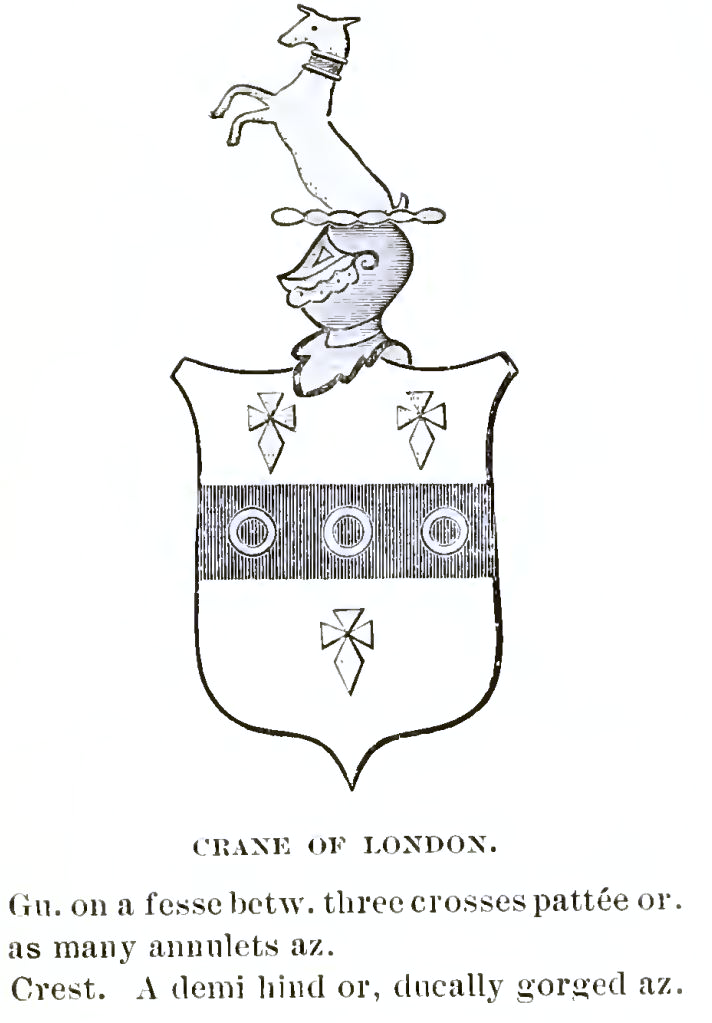
\includegraphics[scale=0.25]{../white/whiteCrest1} 
    \vspace{4ex}
  \end{minipage}%%
  \begin{minipage}[b]{0.5\linewidth}
    \centering
    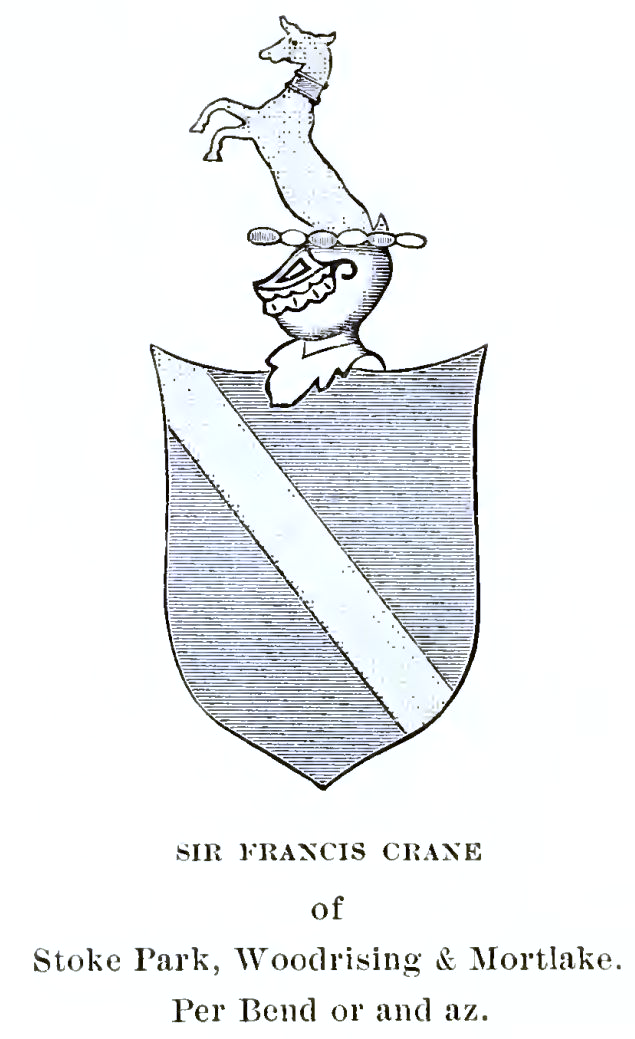
\includegraphics[scale=0.25]{../white/whiteCrest2} 
    \vspace{4ex}
  \end{minipage} 
  \begin{minipage}[b]{0.5\linewidth}
    \centering
    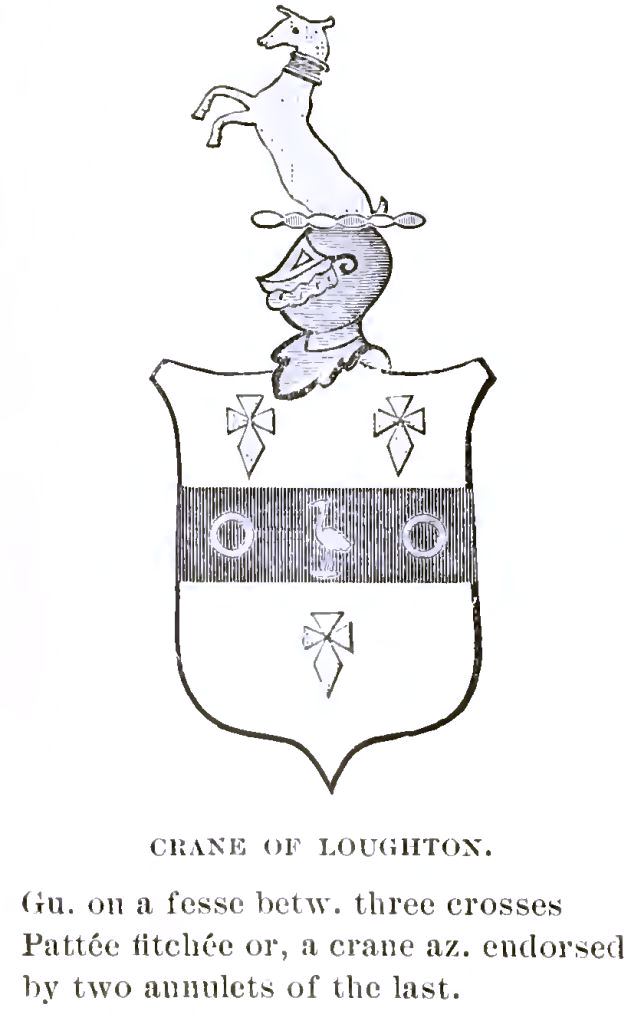
\includegraphics[scale=0.25]{../white/whiteCrest3} 
    \vspace{4ex}
  \end{minipage}%% 
  \begin{minipage}[b]{0.5\linewidth}
    \centering
    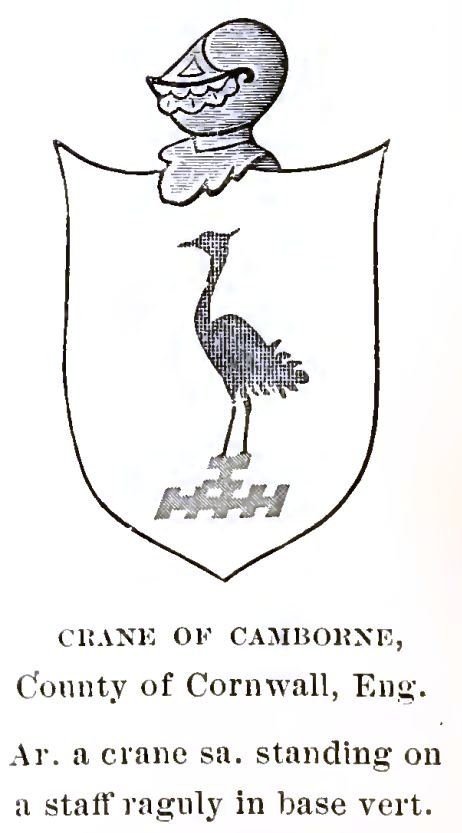
\includegraphics[scale=0.25]{../white/whiteCrest4} 
    \vspace{4ex}
  \end{minipage} 
\end{figure}


\chapter{CRANE FAMILY ARMORIALS.}


For mauy centuries coat armor has been used in England as a 
mark of honorable distinction among families whose representa- 
tives, back in the dim and misty historical past, rendered gallant 
or meritorious service to the crown, and for such service received 
in return a reward of merit or a coat of arms. These armorials 
have been placed on record, and are held as the absolute prop- 
erty of the family to whom they have been assigned. According 
to the laws of heraldry in England no person is entitled to bear 
arms without a hereditary claim by descent or a grant from the 
proper authorities. The use of a crest even is prohibited, and 
the bearer is subject to an armorial tax. Guillam, who is excel- 
lent authority on heraldry, says : " The right to property could be 
established by finding on the premises any known or recorded 
coat armor, and if any man be convicted of treason for betraying 
his country or of heresy to the end he should be branded with 
infamy, his arms are broken down and utterly defaced, and in 
the event that the last of a noble family should die leaving no 
issue, so that there is left no legal bearer of the family arms, the 
arms are placed in the grave with the deceased." It is also 
claimed that the coat of arms is stronger proof of the relationship 
of families than the names themselves, for names were instituted 
to distinguish persons, and in the early use of them brothers suc- 
ceeded to entirely different patronymics. Many families although 
bearing arms do not possess mottoes, and the several Crane family 
armorials that have come to our notice have been lacking in that 
respect, still one member of our family, a native of Cheshire 
County, England, on noticing his neighbor Corbett's motto, 
" Dea.H pascit corvos," "God feeds the' crows," wrote the follow- 
ing for his motto: " Qui pascit corvos non obliviscitur gras," 
' He who feeds the crows will not forget the cranes." At least 
three Crane family armorials have found their way to New Eng- 
land. One of them seems to serve as a connecting link between 
the Cranes of Old and New England. Kate E. Crane, in whose 
hands it was found some years ago, is a granddaughter of Col. 
Jonathan Crane, who was l)orn in 1747. This armorial can be 
traced in the family for more than one hundred and fifty years, 
and Miss Crane was confident that it has been preserved in the 
family since their arrival in this country. Col. Jonathan, through 
whose hands the coat of arms came down, was son of Joseph, 
who was great-grandson of Benjamin Crane of Wethersfield, 
brother of Henry, whose descendants we have attempted to 
record in this volume. 

This armorial, which 'you will iind opposite the title-page, is a 
copy of that of the Suffolk County family, England. The mant- 
ling or lambrequins as well as the ornamentations under the 
escutcheon, however, are not mentioned in the printed description 
of the ancient armorial and are quite immaterial, doubtless put 
there merely to help out the picture. It is described in heraldry 
as Argent,. a fesse between, three crosses crosslet titchee Guls, 
crest a crane ppr. The Cranes in England have borne five coats 
of arms, whether all were originally of one family it does not 
appear, although there are reasons for believing that they were, 
receiving special grants for special service. 

The frontispiece belongs to the Suffolk County family. 

No. 1. The Cranes of London., or that of John clerk of the 

No. 2. Crane of Stoke Park, Woodrising and Mortlake. 

No. 3. Crane of Longhton. 

No. 4. Cranes of Camborne., County of Cornwall. 

In regard to the armorials that have come across the water, the 
one found in the possession of Miss Kate E. Crane the reader is 
already familiar with. Another, similar to No. 3, is a copy of 
the Cranes of Loughton and was found with a Crane famil\}' in 
New Orleans, La., during the war, by the brothers of Hattie R. 
Crane of Collinsville, Conn., who sent the description' to the 
writer. 

Another, similar to No. 1, was used by the Cranes of Nova 
Scotia, descendants of Benjamin of Wethersfield, Conn., through 
Silas Crane who went there from Lebanon, Conn., about the 

Also another, said to have been granted to Sir Joshua Crane in 
1647, and taken from an old cutting found in London, Eng., by 
Mr. John Wells Crane, then a citizen of Paris, France. Copies 
of which were brought to this country by Mr. Waldworth Douglass
Crane of Philadelphia, Pa., some years ago, and is also similar 
to the arms of Craue of Loughton. 

An attempt has been made in producing the cuts of the four 
Crane armorials that appear on a foregoing page to have the lives 
represent the various colors according to the rules of heraldry, 
and the heraldic description is also given under each of them. 
But for convenience of the reader might here add in explanation, 
that the shields of Nos. 1, 3 and 4 are silver, while that of No. 
The crests on 1, 2 and 3 are a demi-hinc' or young deer, also in 
gold, which represented the office of Steward to the King. The 
fesse or horizontal band was red, while the annulets or rings and 
the bird were blue. The crosses gold. In No. 4 the bird is 
black, standing on a staff in base, green. 



\chapter{ORIGIN OF THE NAME CRANE.}


In common with other family names, great latitude has been 
taken in the spelling of our patronymic. The records in New 
England disclose the following styles : Crane, Cran, C'ranne, 
C'rain, C'raine, C'rayne. During the early period of our colonial 
settlements it often occurred that men were ushered into i)u1)lic 
ottice who certainly were, to say the least, adept spellers. lUit 
if judged by the present educational standard wonld be char- 
acterized as somewhat defective in their orthography; nevei-- 
theless they served their time and generation, making good and 
valuable citizens. It is not very many generations ago that the 
man who could write his name was the exception rather than the 
rule, l)ut we are now well past that period of our national history. 
Henry Crane could and did write his own name, and in the man- 
ner it is most commonly spelled, Crane. Careful investigalions 
in the Doomsday Book of England, a record covering the ];eriod 
from 1066 to 1086, have thus far failed to disclose our sur- 
name, and it is not until the year 1272 that we find it, in com- 
mon with other Norman family names, in the record publication 
styled liotull Hutidredormn. There, among the tenants of Sir 
AVilliam le Moyne, a Norman lord, we have Andreas, John, 
Oliver and William de Crane, the de undoubtedly conveying the 
intelligence that tliey were of or from Crannes in Maine, an 
ancient province in France. Thereby furnishing excellent reason 
for the assumption that the Cranes of England were of Norman 
extraction, and that they kjcated there at the time of the conquest 
or not long thereafter. Family names or surnames were not in 
general use previous to the Conquest, and their popularity was 
measured by an exceedingly slow growth. It was only when it 
became necessary to distinguish persons bearing the same Christ- 
ian name, then the only customary name, that it was found need- 
ful to add the second one, and the latter was suggested by some 
prominent characteristic or peculiarity of the person, his occupa- 




tion, or from the locality in which he lived or came from, or possi- 
bly it might be from some natural object. 

Many have supposed that our appellation came within the class 
last cited, for it has been so classed by writers on surnames. It 
doubtless was the easiest way for them to dispose of the subject. 
To be sure, members of the family have used the bird about their 
coat armor, but it was not only proper, but in the line of custom, 
that they should adopt a crest that would be the most appropriate 
pto the family name, and the Crane would certainly not be inap- 
propriate. 

It seems, however, possible and quite probable, that the source 
of one may also disclose the origin of the other. In the Dooms- 
Aay Book, before referred to, are to be found the following 
named places : Craneforda, Cranesford, Cranesforda, Cranesfor- 
dam, Cranewarda, Cranewisse, Cranefort, Cranawarda, Cranlea, 
Cranslea and Cranbone ; nearly all these names appear within the 
Counties of Norfolk and Suffolk, the very localities to which we 
trace the origin of our family pedigree. These words or rather 
names* are from cran, meaning water, and /ord, a shallow place, 
or a village by the ford, stream or lake. These words have for 
their root the Gaelic word an, water, with the prefix cr. We 
have cranmere, a water source or marshy place, also Crane, the 
name of a stream in the southerly portion of the County of Kent, 
England. 

In consulting ancient maps, bearing dates from the year 11 HO 
down to the present period, the town of Craon can be located 
within the province of Maine. This may not be the place referred 
to from whence Sir William and his associates went to England 
some seven or eight hundred years ago, yet it is quite certain that 
they went, from near that locality in France, and it may he the 
very town, surely it is located on the banks of the river Oudin or 
Oudon,* and the name has the same Gaelic root, and signifies a 
place by the water or stream. In the northern portion of France 
we find the name Cranne also located on a stream, and there are 
many other names to be found in this portion of France that 
would illustrate the point, so that there appears little doubt as to 
the origin of our patronymic. It is a loccd name from Crannes 
or Craon and has for its root the Gaelic cran or an, water, and 
the bird doubtless received its name also from being a frequenter 
of brooks or ponds of water and wet, marshy places. 

* Spelled both ways, and Oudiu is a family name. 




Other iiistauces may be fouud where the name has been used 
for a locality.* Cranae, an island of Laconia, and its inhabitants 
were called Cranates. Cranaus, a town of Caria, and there was 
a king of Athens bearing that name who succeeded Cecrops. 
Cranea, a small country of the Ambraciotji?. Crane us was the 
first king of Macedonia. Crania., the ancient name of Tarius in 
Cilicia. Crane, a city of Arcadia in ancient Greece, and it is 
quite likely that with the successive movements of population 
from east to west, which for many centuries continued throughout 
southwestern Europe during those ancient periods, the old local 
names, in a greater or less degree, were brought into use, 

Roger de Mortimer, William de Warrenne' William de Tracy, 
Ralph de Percy, are also local names. Roger was descendant 
from the barony of Mortimer in Normandy, William Tracy was 
from the castle and barony of Tracy in Normandy, while the 
names of Warren and Percy are found in the same class, with 
many others. But it does not seem necessary to multiply illustra- 
tions. It would thus appear that the name has no special refer- 
ence to the bird, that the name of the place, as well as the bird, 
may have been suggested by location and habits. While the 
family name is taken from the place from whence their representa- 
tives emigrated to England. 

A few members of our family write their names Grain or 
Craine ; in is termed one of the diminutive endings, and would 
imply a very small stream, rivulet or streamlet. In a dictionary 
published in London in 1627 we find cranie or craine or cleft, 
to cleave, divide, possibly a narrow opening, a cranny or crannie. 
In many instances the prefixes and also the sufltixes to the root 
an in Gaelic indicate whether the water or stream be clear, deep, 
shallow, stagnant or swift running, and when it stands for the 
name of a place, whether its location be at the source, confluence 
or outlet of the stream. 



' Cole's Dictionary. 



\chapter{CRANE FAMILY IN ENGLAND}



The Crane.s in England are classed among the families belong- 
ing to the County of Suffolk. Numerous families bearing the 
name have been found residents of other counties in Great 
Britain, but it is among the records of Suffolk County that we 
find delineated the long roll of aristocratic landholders in a line 
of succession from father to son covering a period of time marked 
by hundreds of, years. Here their estates are to be found recorded 
which have been retained in the family for nearly 300 years, 
beginning with the fifth year of Richard II., A. D. 1382, at 
which time William Crane of Stowmarket married Margaret, 
daughter and co-heir of Sir Andrew Butler, Knight, by whom he 
came in possession of Chilton in the Hundred of Stow. A number 
of pedigrees of this branch of the family may be found recorded 
in the Harleian Collection, British Museum, London, England, 
reference to their numbers is as follows: 155, fo. 34; 1103, fo. 
2; 1177, fo. 7; 1449, ff. 13, 88 ; 1484, fo. 42 ; 1560, ff. 8b, 17Gb. 
One of Crane of Camborne, County of Cornwall, 1079, fo. 8 ; also 
several of the family of Crane of Loughton, Buckinghamshire, 
1102, fo. G9b; 1151, fo. G.sb ; 1193, fo. 69b; 1234, fo. 51 ; 1391, 
fo. 73b; 1533, fo. 157b. The pedigrees here referred to were 
collected by officers commissioned by the crown for this special 
work. They were called Heralds, whose mission it was to make 
periodical visits over the territory assigned them for the purpose 
of recording the arms, pedigrees and marriages of the nobility 
and gentry within their respective districts. These records were 
preserved, and are known in England as the Herald's Visitations. 
The very earliest of them were made just after the close of the 
first quarter of the sixteenth century, and the custom was con- 
tinued for little more than a century and a half, the latest com- 
mission issued bearing the date of May 13, 1686. In many 
instances pedigrees were noted down as given, and were doubt- 
less believed to be correct by the informer ; but as it was pre- 
sented without documentary evidence opportunity was left for 




considerable variation in returns for the same family. But not- 
withstanding the errors or discrepancies that have been found in 
those manuscripts, they constitute a most valuable historical and 
genealogical record, and form tlie principal source of evidence 
establishing the hereditary right of persons in England to bear 
arms, and also in many cases furnish untold satisfaction to the 
patient student of family genealogy. 

The Crane family pedigrees that have been refoi-red to in the 
Harleian Collection for Suffolk County were collected in the years 
1561-1.577, 1611, and are intended to delineate tlie line of heirs of 
the family of Chilton, covering a period of from six to twelve gen- 
erations ; although they do not entirely agree in every particular, 
it can be readily seen that the heirs follow in the same general 
order. It appears by an examination of these pedigrees that this 
long chain of heirs had its origin in the County of Norfolk, some 
five generations prior to its settlement at the little village of 
Chilton, near Sudbury ; and in order to begin at the end most 
remote we must turn to the MS. for the County of Norfolk. 
Here, in No. 1552, fo. 183, we find the beginning or starting point 
for our Suffolk family pedigree. Although copies of the first men- 
tioned pedigrees have been obtained from England at considera- 
ble expense, we omit their publication here to give place for the 
one last referred to, it being, perhaps, the most accurate and 
complete. 

It begins with Sir Thomas Crane, ' Knight, who married Ada, 
sister to Giles de Kerdiston, and the line of descent proceeds 
through their sou and* heir, Sir Thomas Crane, ' who married 
Petronella Bettesley and had three sons, Richard, Clement, John, 
and a daughter Alice, who became the wife of Sir Edmond Berry, 
Knight. Richard Crane, ' eldest son and heir, married and had 
John C'raiie," wlio married Alice, daughter and heir to Sir 
Edmond Berry 1)v Alice, daughter and heir to Sir Joiui Jerl)ridge. 
Knight. The result of this union was two sons, Symond. Adam 
and a daughter Alice, who married first a Mr. Briggs and second 
.lohn Davis. Adam Crane" married and left Elizabeth, only 
daughter and heir. Si/jiiond Cnnir,-' heir of .lolni. mai'ried 
Margery Smallwood, and had Wil/iinn. C/vom\\" wliost' wives wei\\' 
Anne, daughter of William Forcey oi- Forrecy, and Margery, 
daughter of Sir Andrew Butler, Kniglit; l)y tlie latter lie liad two 
sons, .lohn, ' and Robert C'/v/z/e,"' who nuirrii'd first, Agnes, daugli- 
ter of Thomas Greene of Creeting, st'cond. a daughter of Thomas 




Shiugleton or Singleton, and was of Stouham and Chilton. They 

had Robert, John, and Agnes, who married Appleton of 

Suffolk. Robert Orane' was twice married : to Katherine, daughter 
of Robert Darcy, by whom he had no children ; and Anne, daugh- 
ter of Sir Andrew Ogard, by whom he had George, who died with- 
out issue. Elizabeth, who was Abbess of Brusyerd, Margery, 
who married Thomas Appleton of Little Waldingfield, County of 
Suffolk, ancestor of the Appletons of Ipswich, Mass. Rol)ert 
Crane' leaving no male heirs the line was perpetuated by his 
brother, John Crane,' who married Agnes, daughter of John 
Calthorpe of Norfolk County. They had Robert, Edward and 
Elizabeth, who married Richard Martin or Marton of Melford. 

P'dward' married Isabell ; owned Stratford Hall ; left a will 

dated March 19, 1558, in which no children are mentioned. 
Robert Crane,' heir of John,' married first, P'lizabeth, daughter 
of Richard Southwell of Woodrising, Norfolk County, by whom he 
had Robert,'" Anthony,'** Dorothy, i' who married Thomas Moul- 
ton or Moultinge of Dereham, Norfolk County, and second, Jane 
White of Pvssex County by whom he had John,'** Elizabeth,'" 
wife of Edmond Markauut of Dunham Hall, Suffolk ; Grisselli" 
or Cryssell, wife of Robert Bogas ; Anne,"' wife of John Sandon, 
also of Ambrose Coole, and Agnes, i" unmarried. Anthony'" 
married first, Elizabeth Aylmer ; second, Elizabeth Hussey. By 
first wife he had Elizabeth, who married Anthony Death of Lin- 
colnshire ; by second wife had Dorothy," wife of Thomas Baxster 
and Mary," wife of Gerard Gore, Loudon. Robert Crarie"' mar- 
ried Bridget, daughter of Sir Thomas Jgrmyn, Knight, and had 
Robert, '1 who died without issue, Elizabeth, " wife, first, of 
Edward Wright, second, Edward Reve, Ursula, " wife of Henry 
Smith, Agnes, 11 wife, first, of John Smith, second. Sir Edward 
Cleere, Knight, Anne,ii wife of Ralph Choppiu, Gent., Bridget," 
wife, first, of F'rancis Clopton, second, John Warberton, Mary," 
wife of, first, Bartholomew Strangman, second, Dudley Fortescue, 
Esq., and Henry Crane," who married, first, Anne, daughter 
Thomas Goodwin, by whom had daughter Rubice or Reuben, 
who married Sir Thomas Harvey, Knight; Henry Crane" was 
divorced from this wife and married, second, Catherine, third 
daughter to John Jernegan or Jerningham, p]sq., of Somerleyton. 
She was widow of Sir Wymond Carew of Snettisham, County of 
Norfolk, who was Knighted Feb. 20, 1546. The fruit of this 
marriage was a son Robert, " born after the death of his father. 




This Robert Grane'"' married, first, Dorothy, dauo-hter of Sir 
Henry HoTjart or Hubart, Knight, Lord Chief Justice of the 
Common Pleas, slie died witliout issue, April 11, 1624; second, 
Susan AlUngton, Sept. 21, 1624, she was daughter of Sir Giles 
Allington of Cambridgeshire. By wife Susan had Susan ,," born 
Oct. 12, 1626 ; died Aug., 1628. Dorothy," born Oct. 29, 1627 ; 
died Jan., 1638. Mary," born March 19, 1629; m. Nov. 26, 
1647, to Sir Ralph Hare of Stow, County Norfolk. Snscm," 
born May 26, 1630. Anne," born Oct. 17, 1631. Giles," born 
Dec. 13, 1632; died May, 1639. Elizabeth," born Aug. 18, 
be noticed that the pedigree given traces the line of heirs for 
thirteen generations, covering a period in the existence of this 
family in England not far from three hundred years. 

As a careful examination of the original Doomsday Book failed 
to reveal the record of a person bearing our appellation, it is 
possible that at the time when that famous survey was made, 
son by the name of Crane. Still it is not by any means certain 
that persons bearing that name were not there, for it is not 
claimed that the Doomsday Book furnishes a complete roll of the 
family names that existed in P'ngland at the time that record was 
made. That our family are descended from the Norman blood 
we are reasonably sure. Our ancestral stock may have been 
represented among the humble followers of William the Con- 
queror when he passed over into England to take possession of 
the government which Edward the Confessor had bequeathed to 
him. They were not all barons and nobles that formed that 
victorious army of the Norman conqueror ; all classes were repre- 
sented. It was, perhaps, a body of men fairly representing the 
Norman people of that period, many of them, it may be, of lium- 
l)le birth, who, through subsequent deeds of bravery and heroism, 
arose by promotion to exalted stations, receiving various marks 
of distinction as a reward for their services. It is claimed that, 
as a class, the Norman people were the most practically intelli- 
gent and energetic race of their age, and the author of a recent 
publication on "The Norman People," says, in addition, that the 
ancestry of the intellectual aristocracy of England was generally 
Norman. This quotation may give a comforting thought to those 
of the family who are sensitive to the value or reputation of ])lood. 
The American people generally have grown to place not so much 




stress ou blood alone, but no doubt the most of our family may 
be willing to accept that for what it is worth. It must, however, 
be conceded that good family blood seldom serves as an embar- 
rassment or obstruction to the formation of true manly character, 
but on the other hand it frequently proves to be the leaven that in 
the end works for good. King William, after he had gained 
possession of the lands in Phiglaud by conquest, and in order to 
better protect his followers in their acquired rights to the soil, 
sent commissioners into each county for the purpose of accumu- 
lating exact statements of the property and revenue of the king- 
dom wherever rents and services were due to the crown. These 
inquisitions or surveys were completed in the year 1 ()(), and 
afterwards arranged in proper order in a record called Doomsday. 
It did not constitute a complete survey of all the land in the 
country any more than it did a census of the entire population. 
Estates that were free from the claims of the crown, as well as 
the names of persons not under obligations or indebted to the 
king were omitted. Through the means of this record we learn 
that estates or manors were managed for the crown by stewards 
or lords as subtenants. Many Normans who had rendered assist- 
ance to the Conqueror were rewarded by being made tenants in 
chief to the king. Of these teyumts in chief there were about 
fourteen hundred in number. They were considered the most 
distinguished men of that period, and stood ready at a moment's 
notice to render any service that the king might require of them, 
whether of a civil or military nature. These lords of the manors 
could sublet to under-tenants of various rank in the boroughs 
where they lived, and known as cottagers, freemen, socmen, ten- 
ant by socage, and villein or bondmen. These numerous ten- 
ants, under their lords, constituted the standing army of the 
king, and furnished not only the defence, but support of the 
crown. From an EngUsh record, bearing date A. D. 1272, called 
Rotuli Iliiiidredoriiin, vol. II., 659, we learn that at that period a 
Norman, Sir William le Moyne by name, was lord over Saltrey- 
Moyne in Huntingdonshire, and that among the sixty-eight tenants 
under him the name of Crane appears. This ancient roll also 
gives the names of Andreas, John, Oliver, and WilUam de Crane, 
evidently taking the name from Crannes, a town then within the 
Province of Maine, from whence they emigrated to England. 

That the Sir Thomas Crane heading the pedigree we have 
quoted, was a son oi' not of one of the above named Normans 




we may never know, but a\\\\ data at hand seems to verify or eon- 
firm the predication that our family is of Norman extraction. 
Whether Ada, the wife of Sir Thomas, was a danoliter or a sister 
of Fulco de Kerdiston or, as the pedigree we liave quoted gives 
it, the sister of Giles de Kerdiston, it matters little, the Norman 
blood would still remain as the fountain head. 

The period at which our family pedigree is taken up would 
carry us back very nearly, if not quite, to the time when the 
record of our patronymic first appears in England. A mere 
record of names of a line of family heirs running down thi'ough a 
space of three hundred or more years, although furnishing evi- 
dence of wealth, rank and titles that have been shared and 
enjoyed by members of the family, it does not fully satisfy the 
curiosity of an American genealogist ; there is too much left out, 
it is not sufficiently complete, the very branches of the family 
tree that he desires most, perhaps, to find have been lopped off l)y 
the wayside, and he must content himself with examining the 
closely shorn trunk. The task of supplj'ing any considerable 
number of these missing branches would be confronted l)y so 
many almost unsurmountable difficulties that it could not lie 
undertaken at this time, but owing to the fact that the policy of 
the English government has been in years past to keep or hold in 
sight, by authoritative records, the proprietors of wealth\}- or 
landed estates for the purpose of drawing revenue therefrom 
whenever needed, we are able -to present to the reader a few addi- 
tional names of members of the family who arose to positions 
worthy of mention. As we turn again to the pedigree of the 
family in England let lis briefly consider the place of its origin 
or geographical starting point. Sir Thomas Crane married Ada, 
sister of Giles and probably daughter of Fulco de Kerdiston. 
The Kerdeston* Manor is situated in the Hundred of Elynesford, 
al)Out two miles northwest by north from Rupham in the County 
of Norfolk, and was in the possession of Tord, a freeman, who 
was deprived of it at the conquest. Geoffrey Bainard is said to 
have held it under his father, Ralph, Lord Bainard at the time of 
the survey ; but Rev. George Munford in his analysis of the 
Doomsday Book of the County of Norfolk, tells us that "William 
de Warren was tenant in capite of this manor, but held only (ne- 
lialf the clnirch. The familv of Kerdiston was earlv ensossed of 



Variously spelled Kerdestone, Cardiston. 




this lordship.* Fiilco de Kerdiston was lord here in the reign of 

For a period of more than a century after the first persons 
bearing our patronymic located in England they, for the most 
part, according to our record, continued to reside within a radius 
of twenty-five or thirty miles of each other. Within the extent 
of such a circle were also to be found the early representatives of 
the famiUes of Berry, Calthorpe, C.arbonel, Ogard, Botelir or 
Butler, and Jerningham or Jeringan, into which the Cranes sub- 
sequently married. John Crane, who married Alice, daughter 
and heiress of Sir Edmund Berry, Knight, was of Wood-Norton 
in the Hundred of Eyuesford, County of Norfolk, seven miles 
northwest of Rupham and within five miles of Kerdiston. Hugo 
or Hugh de Norton was early in possession of this manor. John 
de Norton was lord here A. D. 1250, and William de Norton A. 
D. 1361, who for some crime fled beyond the sea and the manor 
escheated to the crown. Nicholaa, the wife of William, married 
John Spoo, and they were in possession of it A. D. 1386. Sir 
Thomas Geney held it in 1401, and John Bryston, Esq., in 1424, 

The above John Crane was lord here A. D. 1428, and by an 
agreement made April 20, 1430, it appears that this John Crane, 
Esq., and Sir Edmund Berry were seized in the fee of Norton 
Hall, also Lyng Hall and their tenements. The records also 
show that Lyng Hall was A. D. 1414 in possession of Joan, relict 
of William Gerbridge, Esq., from whom it passed to the above 
John Crane, who presented it to All Saints' Church, as lord of the 
manor, in A. D. 1427. He also presented to St. Peter's Church 
the following year, as lord of, the manor of Norton Hall, there 
being two consolidated parishes in the village of Wood-Norton. 
In the year 1457 Alice Crane, presumably widow of John, pre- 
sented with Edmund Docking and Margaret, his wife, each. 
Crane and Docking, holding a moiety of presentation in, Lyng 
Hall to All Saints' Church. John Crane, Esq., of Wood-Norton, 
conveyed in 1437 to William Oldhall a moiety of the manor of 
Ilney, and two parts of the manor of Yaxham, which was the 
Gerbridge Manor. About the year 1473 Hugh Gerbridge was 
lord here and the manor was divided into two parts. Crane held 
one which he sold to Henry Stunner. Ilney was also divided 
into two parts, and Crane sold his to Stunner. In 1547 Richard 
Southwell held this manor and it fell into the hands of the Cranes 



Blomefleld History, County Norfolk. 



and Claytons. The family liad noAV liecome quite numerous in 
England, the greater number of them, perhaps, residing in the 
County of Norfolk. In 1416 John Pyke, late prior of the Holy 
Trinity of Ipswich, granted to John Crane and Roger Cottemower 
his manor of Minyots, paying yearly to the Church of St. Marga- 
ret's of Seething six marks. There was also a John Crane of 
Tilney, a yeoman, who made his will June 30, 1583, in which he 
mentions a sister Joan Peers, a brother Walter and wife Margery, 
children Margaret, Cyprian, Thomas, and John who was to have 
at the age of sixteen j'ears ten pounds yearly until he reached 
the age of twenty, then he was to have all lands, etc., in freehold 
and copyhold in Tilney, Islington, Wigenhall, and Terriugton 
forever, also the lease of Hilmoredikef Robert Crane of Wymond- 
ham, draper, gave by will, dated 28 May, 1620, to wife Margery 
house and tenements called "The Griffin," with other houses and 
lands, both freehold and copyhold, for life ; son Richard to have 
a copyhold estate of ten acres near Fiffard Bridge in Wymond- 
ham, and what his mother may leave ; also mentions son Thomas, 
daughters Johane, Elizabeth, Anne, and Frances, each receiving 
thirty pounds on becoming of age. 

But among the most prominent of the family in the County of 
Norfolk was Sir P'raucis Crane and his brother Sir Richard, both 
of Woodrising. Whether they were natives of the county or not 
the writer is unable to state, but there are many reasons for 
l)elieving that they were descendants from some of the earl\}' 
families there. Sir Francis was secretary to Charles I., Prince 
of Wales, and Knighted at Coventry, Sept. 4, 1617, by King 
James I., father to the Prince. He was also made Chancellor of 
the Order of the Garter, a mark of special and rare distinction. 
The emblem of the order is a dark ribbon edged with gold, 1)ear- 
ing the motto, "'Honi salt qui mal y x>ense," * in golden letters, 
with a buckle and pendant of gold richly chased, and is worn on 
the left leg below the knee. The mantle is of blue velvet, lined 
with white taffeta, and on the left breast a silver star is embroid- 
ered. The hood and surcoat are of crimson velvet, lined with 
white taffeta. The hat is of black velvet, with a plume of white 
ostrich feathers, in the centre of which there is a tuft of l)lack 
heron's feathers, all fastened to the hat by a band of diamonds. 
The collar is of gold and consists of twenty-six pieces, e:icli in 
the form of a garter. 

* " Accursed be he who thinks there 's evil in it." 




.Sir Francis in the year 1611) introduc3d into England tlie man- 
ufacture of curious tapestry and, with the assistance of King- 
James I., who contributed two thousand pounds towards the 
enterprise, built a mill at Mortlake, then a village on the river 
Thames in the County of Surry, about nine miles distant and in 
a westerly direction from London. This mill contained three 
rooms, one twenty feet in width by eighty-two in length, in which 
were set twelve looms, the second room was half the size of the 
first and contained six looms, the third was called the " Linning 
Room." He engaged workmen to come from the tapestry works 
at Paris, France, and from other parts of Europe, employing the 
highest skilled labor that was at that time to be obtained. To 
accommodate his Flemish ttipestry weavers he, on the 20 March, 
1()21 (O. S.), secured a license from the Archbishop of Canter- 
Iniry for them to assemble for worship in the parish church of 
Mortlake, at his house or in any other suitable place, and arranged 
that a minister and an elder should be sent out from the Old Dutch 
Reform Church, Austin Friars, in London, when necessary to 
perform the service. July 8, 1623, for the encouragement of the 
work, King James I. wrote to the King of Denmark asking that 
Francis Cleyne, a painter and native of Rostok, a town in the 
Doutehy of Mecklinbourgh, might be allowed to come to England 
for the purpose of being employed as a designer at the Mortlake 
Tapestry Works. About the close of the year Mr. Cleyne arrived 
in London with his family, and was immediately called into ser- 
vice at Mortlake. The success of the work was now doubly 
assured and great progress in the art of weaving rare and beauti- 
ful designs in tapestry was achieved during the years that followed. 

At the death of King James I., March 27, 1625, his son Charles 
I. ascended the throne, and during the first year of his reign became 
indebted to Sir Francis £6000 for three suits of gold tapestry. 
Through the assistance of Francis Cleyne Sir Francis succeeded 
in manufacturing many historical and grotesque pieces of gold 
tapestry, and the records state that the work was carried to singu- 
lar perfection. The five cartoons of Rafaele were copied in tap- 
estry and put up in Hampton Court, where they were to be seen 
in 1884. A suit of hangings, representing the five senses, were 
in the palace at Oatlands, and sold in 1649 for £270. The beauti- 
ful liangings at Houghton, Lord Orford's seat, containing whole 
length ])()rtraits of King James, King Charles, their queens, and 
the King of Denmark, with heads of the royal children in the bor- 



(HANK KAMILV IN EN(iLANI). "29 

(lers, are said to have been mamifactured at 'Nlortlake. Williams, 
Archbishop of York and Lord Keeper, paid Sir Francis £25U0 
for the four seasons. At Kuowl, the Duke of Dorset's, in Kent, 
there was in 1814 a piece of silk tapestry containing portraits of 
Vandick and Sir Francis Crane himself. In 1634 he was chosen 
one of a commission to purchase a tract of land to be used by 
King Charles I. as a game park. For seventeen years he was 
given by the King exclusive privilege of making copper farthings 
for circulation, at the yearly rent of one hundred marks payable 
into the exchequer. He contributed f 50U tOAvards the building 
of St. Paul's Church iu Loudon. 

This Sir Francis Crane has been styled as of Surry, on account 
of his tapestry works at Mortlake, and also of Northamptonshire, 
because he owned lands in that county. But he called himself of 
Woodrising, County of Norfolk. He married Mary, daughter of 
David and sister of Sir Peter de la Maire. He made his will 
Aug. 27, 1635, ])y which he gave to wife Dame Mary lands in 
Northampton and other places, and to brother-in-law Sir Peter la 
Maire iu trust to found five dwellings for five poor knights at 
Windsor; names his brother Richard Crane sole executor and 
heir to all his property. In a codicil, dated Paris, June 23, 1636, 
he expressed a desire to be buried at Woodrising. He died there 
three days later, leaving no children, and was buried at Wood- 
rising on July 10. His brother Sir Richard, who came in posses- 
sion of the tapestry factory at Mortlake, assigned it to the crown 
and retired to the Manor of Woodrising, also bequeathed to him 
by his brother. He was created a baronet March 20, 1642, and 
also knighted b\}' King Charles I. at Chester, September 26, same 
year. First wife was Mary, daughter of AYilliam, Lord Widdring- 
ttni, and after her death he married Jane , but left no chil- 
dren by either marriage. At his death, in 1645, by his will, 
Sept. 20, 1645, the manor passed to his adopted heiress and niece, 
Frances, youngest daughter of his sister Joan Crane, who became 
the wife of William Bond, of Earth, in the County of Connvall. 
Frances Bond married William Crane of Loughton, son of John, 
Clerk of the Kitchen to Kings James and Charles. AVilliam 
Crane and wife Frances sold the Manor of Woodrising iu Kills to 
Gabriel Bedle, citizen and stationer of Loudon. No elfort has 
been made towards furnishing, at this time, a complete list of the 
Cranes of Norfolk C-ounty, for they were at one time quite numer- 
ous in that portion of England, and as one generation after 




fiiiotlier came forth to face the necessities and responsibilities of 
life they became scattered about, finding new homes in other 
counties, some of them quite remote from the spot where the 
family name was first established. 

Several of the family early made their way into the neighbor- 
ing County of Suffolk. The year 1417 found a John Crane in 
the parish of Coddenham, situated not far from the centre of the 
county, and it is possible that some of the family may have estab- 
lished homes in this county even earlier than that period, but 
William Crane, who married Margery, daughter of Sir Andrew 
Butler, Knight, is the first person mentioned in the line of our pedi- 
gree (previously quoted) who settled in Suffolk. He was styled 
of Stonham and Creeting, villages in close proximity to Codden- 
ham. Their son Robert inherited through his mother the Manor 
of Chilton, situated near the southern boundary of the county and 
within less than two miles of the flourishing town of Sudbury. 
Here for more than two hundred years the Cranes remained lords 
of the Manor of Chilton Hall. Mr. William S. Appleton of 
Boston, Mass., who traces his ancestry to this branch of the 
Crane family, and who, after making a personal and careful 
examination of the records in England relating to this family, 
published a unique volume entitled, "Memorials of the Cranes of 
Chilton," in which he gives some very interesting statements con- 
cerning the family, including several pedigrees and illustrations, 
with full descriptions of the tombs and memorial tablets that 
were erected by members of the family in the parish church dedi- 
cated to St. Peter in honor and memory of Robert Crane and 
Lady Arundell, his wife, also Sir Robert Crane and wife Dorothy, 
daughter of Sir Henry Hobart of Blickling, in the County of 
Norfolk, Knight and Baronet, sometime Lord Chief Justice of 
Common Pleas. A more complete illustration of the latter monu- 
ment, however, may be found in Vol. I. of the "Visitations of 
Suftolke," edited by Joseph Jackson Howard, LL.D., F.S.A., in 
which also may be found some thirty pages devoted to the publi- 
cation of pedigrees, wills, extracts from parish records, etc., 
relating to the Crane family. In making up the narrative con- 
cerning this branch of the family advantage has been taken of the 
contents of that volume, as well as other data, including extracts 
from wills that have been copied expressly for the purpose of 
aiding in the compilation of this work. Robert Crane, the son 
and heir of William, above mentioned, resided at Chilton and left 




a clauiihter Agnes, who married Appletoii ; sons, Jolni and 

Robert, the latter became heir to his father's estate and married, 
first, Katherine Darcy, who died childless ; second, Anne, daugh- 
ter of Sir Andrew Ogard of Buckingham," County of Norfolk, 
Knight. He died Oct. 23, 1500. She was widow of Sir Renfrey 
Arundell, Knight ; the result of this union was three children : 
Greorge, who died 1491 without issue; Elizabeth, who became 
Abbess of Brusyerd ; and Margery, who married Thomas Apple- 
ton of Little Waldiugfield, and from whom are descended the 
Appletons of Ipswich of Mass., U. S. A. 

After the death of Greorge, the only son of Robert Crane' of 
Chilton, the latter made his nephfew, Robert,' son of his Ijrother 
John Craiie' of Stonham, heir to his estate at Chilton. This 
Robert' married, first, Elizabeth, daughter of Richard Southwell 
of Woodrising, County of Norfolk, who left three children : 
Robert, 10 Anthony, i" Dorothy i ' ; after the death of E'lizabeth he 
married Jane White of Essex, by whom he had John,!" Elizabeth, "' 
Anne,'*' Gryssellii*' and Agnes, i*' By will dated the 27 of Eeb- 
ruary in the ' ' fourth year of the most gracious reign of Edward 
\\T.," we learn that after providing for special gifts by various 
sums of money to five of the children, and in addition to Anthonyio 
" one annuitee of tenne marks yerely " during his natural life, and 
certain sums to be distributed among the poor of the parishes of 
Newton, Great Waldiugfield, Acton, Great Cornard, the three 
parishes of Sudbury, and among every household in Chilton. The 
residue of all his goods, movable and immovable, he bequeathed 
to his son Robert, i*' who was to be sole executor and he to answer 
l)efore God at the last day for the faithful performance of the trust. 
Anthonyi" married, first, Elizabeth Aylmer ; second, IClizabeth 
Hussey. He was cofferer to Queen Elizal)eth, and dying in Lon- 
Aug. and proved 9 Sept., 1583. He left two daughters, ICliza- 
beth,ii who married Anthony Death of Lincolnshire, and Mary,i' 
who liecaine the wife of Gerard Gore, whose father was alderman 
of London. Dorothy" married, first, Thomas Mantinge of Dere- 
liam, County of Norfolk ; second, Thomas Baxster. Elizabeth"' 
married P'dward Merchant. Annei*' married, first, John Saiiden ; 
second, Ambrose Coole. Gryssell'" became the wife of Robert 
Bogas. Robert Crane' died previous to Aug. 5, 1551, and his 
son and heir, Robert Crane, i" married Bridget, sister to Sir 
Ambrose, amL daughter of Sir Thomas Jermyn, Knight. By a 




will executed October 7, 1590, by the last luuned Robert Crane, 
we learn that he was born about the year 1508 ; that the death of 
his wife Bridget had recently occurred, as well as that of Henry, ' ' 
his only son and heir apparent. This Henry, i' however, left a 
son Robert,!' who by this will was to receive, on reaching the age 
of twenty-one years, substantially the bulk of his vast estate, 
which was of no mean proportions. It consisted of some fourteen 
manors or farms situated within the confines of twenty-one or 
more different parishes in the central and southern portions of the 
County of Suffolk. The young heir at the time of the execution 
of his grandfather's will being but about three years of age gave 
abundant opportunity for others* of the family to derive considera- 
ble benefit from the use of the estates before the grandson could 
arrive at the legal age as property holder ; consequently Robert 
Crane" devised it somewhat in this wise : the manors of Creeting 
St. Olive, called Woluhall or Wouhall, and Minetts, alias Min- 
cotts, with the appurtenances holden of her Majesty in chief, the 
advowson of the Church of Creeting St. Olive and the manors or 
farms called or known by the name or names of Thedwardes, 
Cookes or Cranes, Bacons or Bakens, with all the lands, tene- 
ments, etc., belonging to said mentioned manors or farms lying 
and being in Creeting St. Olave, Creeting St. Mary, Creeting All 
Saints, Earl Stonham, Stonham Aspall, G-osbeck, Coddenham, 
Crowfield, Mickfield, Bayleham, Barking and Brettenham were to 
be occupied and held in trust by his daughters Anne, wife of 
Ralph Choppin, and Dame Agnes, wife of Sir Edward Cleere ; 
gibbes at the barn and all lands, etc., in Acton not a part of the 
Manor of Waldingfield Hall, and in the towns of Melford, Great 
Cornard, Little Cornard was to be used and occupied by Thomas 
Smyth, son of his daughter Ursula, she being dead; the Manors 
of Fledhall and Waltam Hall and appurtenances with freehold 
and charter-lands, etc., being and lying in Little Stonham and 
Mendlesham were to be held by Robert Reve, son of his daughter 
Elizabeth, she being dead. This Robert Reve was also to come 
in possession of Chilton in case young Robert should not live t<j 
reach the age of twenty-one. The manor or farm called the 
Marshes, lying in Creeting All Saints and other towns adjoining, 
and all other lands or tenements of whatsoever description, not 
otherwise disposed of, were to be placed in the possession of Sir 
Robert Jermyn, Knight, whom he especially appointed guardian 
of the young heir, that the proceeds of same migjit be used for 




the purpose of giving young Robert a virtiunis education and a 
Godly bringing up. The Manor of Morereves in Waldiiigfield, 
which he held l)y copy of court roll, was during the minority of 
the young heir to go to the use of JMary, his daughter, now the 
wife of Dudley Fortescue. The Manor of Chilton was also to 
remain at the use of this daughter Mary and her said husband, 
and they to occupy his mansion house at Chilton until said 
Robert'- come of age. The ]Manor of Eav\\ Stonham, which 
was held by copy of court roll, with the appurtenances, was to go 
to the use of the aforementioned Robert Reve. Catherine, widow 
of his deceased sou Henry, is also provided for during her life- 
time, and all the leases are bound to Sir Robert Jermyn, Sir 
Philip Parker, Sir William Spring, and Sir John Heigham, 
Knights, for the faithful performance on their part of every obli- 
gation imposed upon them by the terms of the will, which is, in 
substance, that after the use of the estates during the minority of 
said Robert Crane" they shall, after doing all needed repairs upon 
the several estates during the terms in which they have held pos- 
session, yield and deliver up said estates to said Robert Crane" 
on his arriving at the age of one-aud-twenty. Two hundred and 
ten pounds was to be equally divided betn'een his twenty-one 
grandchildren. All the tools and farming implements, and house- 
hold goods, furniture, horse-mill, etc., about his mansion house 
at Chilton or elsewhere were to be inventoried and an account 
rendered for the said Robert when he should come of age. For 
the better preservance aud safe-keeping of all records, papers, etc., 
and for the better accomplishment of his good intent, a chest or 
" presse " was to have been provided with a lock, and each executor 
with the supervisor to have a key. His gold chain and signet of 
gold was also to be kept in the chest and go to said Robert Crane" 
at the age of twenty-one, and should he die under age the chain 
and ring were to go to Robert Straungman, from whose father the 
chain was purchased. He gave forty shillings to the poor people 
of Great Waldingfield and Chilton, three pounds to the poor peo- 
ple of Sudbury, forty shillings to the poor of Long Melford, 
twenty shillings to the poor of Acton, and the same amount to 
tlie poor people of Newton. Each man servant engaged in his 
employ at the time of his death was to receive the sum of twenty 
shillings, aside from their just dues. Dudley Fortescue and 
cousin Thomas Appleton, Esq., executors, with Mr. Justice 
Clenche supervisor. The young heir had the good fortune to sur- 




vive the allotted period and receive the valued possession. Sir 
Robert Jermyn of Rushbrook, Knight, in whose family young 
Robertas was reared, no doubt was faithful to his trust, no pains 
having been spared in giving the young heir a reasonable educa- 
tion, one that, as subsequent events proved, enabled him to take 
high and responsible positions among the people of his own neigh- 
borhood, and at last elevate him to a seat in the House of Parlia- 
ment. Before he was out of his teens honors began to be laid 
upon him, a fact that furnishes sufficient evidence of a certain 
amount of worthiness and high social standing that placed him 
among the favorites of King James I., who conferred upon him 
the order of Knighthood at Newmarket, Feb. 27, 1604-5. About 
two years afterwards, Jan. 19, 1606-7, he married Dorothy, 
daughter of Sir Henry Hobart, Knight, Lord Chief Justice of the 
Common Pleas, and soon came in possession of the extensive 
estates left him by his grandfather, taking up his residence at the 
old family mansion, "Chilton Hall." William S. Appleton, 
Esq., in his narrative, tells us of his being on terms of intimate 
friendship with the Appletons of Little Waldingfield and the 
Winthrops of Groton, and quotes from the diary of Adam Win- 
throp an invitation, under the date of Oct. 4, 1608, for himself, 
wife, and daughter to dine with Sir Robert Crane at Chilton, and 
that his coach was sent to bring them. Mr. Appleton also 
informs us that King James I., by letters patent, on the 22 of 
Nov., 1615, granted to Sir Robert Crane "Free Warren" in his 
extensive estates, which was giving exclusive privilege to keep 
and hunt certain beasts and fowls within the confines of his 
estates. The original charter, bearing the portrait of the king, 
was, in 1868, in the possession of Mr. Appleton. In the year 
of the County of Suffolk as one of the two candidates for ' ' Knights 
of the Shire." At this election, which occurred in the month of 
December, he was successful, and at once made himself conspic- 
uous as a member of Parliament, joining that body at its session 
which convened 50 Jan., 1621. His manifest faithfulness and 
thorough devotedness to the best interest of his constituents, 
together with the earnest zeal he displayed for the welfare and 
prosperity of the country in whose service he labored, brought 
him many renewals of the confidence reposed in him by the inhabit- 
ants of his district. The next election gave him a seat in Parlia- 
ment as a representative from Sudbury. April 11, 1624, his wife 





Donttliy (lied, and he married 21 Sept., foll()win<>-, Susau, dauuhter 
May, 1 627, he was created by King Charles I. a Baronet. In l(i.'32 
he was High Sheriff for the County of Suffolk. At the election 
in 1640 there arose a question whether Mr. Brampton Gurdon,* 
who claimed he had been chosen, or Sir Robert was entitled to 
the seat in Parliament. Oil the eighth of the month of December 
Mr. Maynard reported the question and a committee was chosen 
to hear witnesses and decide the case. After due consideration 
they reported "that Sii* Robert Crane is duly elected." This 
decision gave him his seat in the famous "Long Parliament," 
where he joined the party opposed to the course adopted by King 
Charles, although it does not appear that he took an active part 
ill the notable struggle. He affixed his name to the Protestation 
of May 3, 1641,t which declared strongly for the Protestant 
Religion and the Privileges of Parliament. By authority of the 
King's most Excellent majesty, and the Lords and Commons 
he was appointed one of the Commissioners for the County of 
Suffolk, whose duty was to attend to the enforcement of an act 
passed by that honorable body for the punishment of scandalous 
clergymen and others. This act begins as follows : "Whereas it 
is the duty of every christian Commonwealth not only to provide 
able and painful ministers for Preaching of Gods Word, whereby 
the Gospeil may be advanced, and mens souls saved. But also to 
l)urge the'. Church of insufficient, scandalous, and idle ministers, 
b\}' home Religion is defamed, the Church scandalized, and the 
souls of men endangered ; And when such are discovered, the 
Remedy ought to be as speedy as possible may be, which of late 
years hath been much neglected, as appears by several informa- 
tions, complaints, and examinations, had, made, and taken, in 
this present Parliament from the several parts of this Kingdome. 
Be it therefore Elnacted by the Kings most P'xcellent Majesty, the 
Lords and Commons in this present Parliament assembled, and 
by the Authority of the same, That the Lord Chancellor or Lord 
Kee[)er of the Great Seale of England, for the*time being, upon 
suit unU) him made in that behalf from time to time, from and 



* Brampton Gurdon was son of John Gurdon of Assington, County 
Suttblk, and in his will bequeathed five pounds to Mr. Rogers of Ipswich 
in New England. He was also connected by marriage to the Saltonstalls. 

t Memorials of the Cranes of Chilton. 




Shall award Commissioners under the Great Seale of England, 
to such persons of worth and credit in every County within the 
Realme of E'ugland, Dominion of Wales and the Isles of Gearnsey 
and Jarsey." Then follows full list of the Commissioners for the 
several counties. Three or more of these Commissioners were to 
constitute a board for the trial of cases, hear complaints, issue 
warrants for bringing before them the accused, who were to be 
tried before a jury of "twelve good and lawful men of the 
county," and also to summon persons who may testify in the 
cases to be heard. The crimes made punishable by this act were, 
not preaching the Word of God at least six times a year by any 
ecclesiastical person under forty years of age having care of souls 
and not hindered by sickness or imprisonment. Blasphemy, 
wilful and corrupt perjury, and subordination of perjury, fornica- 
tion, adultery, common alehouse or tavern haunting, common 
drunkenness, common profane swearing and cursing, done or 
committed within three years now last past before the first day of 
this present session of Parliament, or that shall be done or com- 
mitted before the first day of November, which shall be in the 
year of our Lord 1645, at which date power to try cases under 
this act was to cease. But whatever was executed in the mean 
time under the act was to stand in law and remain in force. 

It will be seen by the following incident related in the Life of 
Mr. Arthur Wilson, then steward to the family of the Earl of 
Warwick, that Sir Robert Crane, Baronet, remained l'aithful to 
the side of Parliament. Mr. Wilson relates that in August, 1642, 
a mob surrounded Long Melford, the seat of Lady Rivers, a 
recusant, and he was sent with some few men and a coach with 
six horses to fetch Lady Rivers to Leeze.* On reaching Sudbury 
he was stopped, and after a time, being recognized by the town 
clerk, was set free, but he could go no further to succor Lady 
Rivers, for there was so great confusion at Melford that no man 
who appeared like a gentleman l)ut was made a prey to that 
ravenous crew. So Mr. Man, my ladies gentleman, and Mr. 
Wilson took horse, leaving the coach at Sudbury, and went a by- 
way to Sir Robert Crane's, a little nearer Melford, to see what 
might be learned about the Countess. By Sir Robert they were 
told that Lady Rivers had escaped to Bury and was on the way 
to London, while he was compelled to retain a trained band in 



* Mr. Appleton says it refers to Lees Priory, near Braintree in Essex, 
a seat of tlie Earl of Warwick. 




his bouse to secure himself from the rabble who threateued him 
for assisting her to escape, although he was a Parliament man. 

Sir Robert was a subscriber to the equipment and maintenance 
of the army. He furnished in the years 1641 and 1642, besides 
a considerable sum of money, two gay geldings for Christopher 
Reps Troope, valued at £30. Four were sent, but two of them 
were returned, the Troope being full, "And in leiue thereof hee 
keepes fower horses for the service and defence of the Country." 

He died at London, Feb., 1643, and on the seventeenth day of 
the same month the House of Commons ordered "that the Lady 
Crane shall have Mr. Speaker's warrant to carry down into the 
country the body of Sir Robert Crane, lately a member of this 
House." The burial took place at Chilton the following day, 
Feb. 18, 1643. By his second wife he had ten children, two 
sons, who died very young, and eight daughters, three of whom 
died before their father and one soon after him. The remaining 
four, Mary, Susan, Anne, and Elizabeth, became his co-heiresses. 

Mary, born March 19, 1629; married in 1648, Sir Ralph Hare 
of Stow-Bardolpb, Norfolk, Baronet, and became the mother of 
seven children. Susan, born May 26, 1630; married 1649, Sir 
Edward Walpole of Houghton, Norfolk, Knight of the Bath, and 
was ancestress of the present P'arl of Orford and of all the famous 
members of the Walpole family; she died July 7, 1667, and 
was buried at Houghton. Anne, born Oct. 17, 1631 ; married 
Aug. 28, 1649, William Airmyne, Esq., afterwards Sir William 
Airmyne of Osgodby in Lincolnshire, Baronet, and left only daugli- 
ters ; after his death she married second, Hon. John Belasyse, 
Baron Belasyse of Worlaby, County of Lincoln, no children by 
this marriage; she died Aug. 11, 1662, and was buried at St. 
Giles in the P'ast, London. Baron Belasyse was a noted military 
commander under King Charles I. and also King Charles II. 
He raised six regiments of horse and foot for the civil wars of 
that period ; took part in the battles of Pxlghill, Newbury, and 
Naseby ; also the sieges of Redding and Bristol ; afterwards was 
Governor of York and Commander-in-Chief of the forces in 
Yorkshire. He fought the battle of Selby with Lord Fairfax, at 
the same time was Lieut. -General of the Counties of Lincoln, 
Northampton, Derby, and Rutland, also Governor of Newark, 
and enjoyed the honor of being General of the King's Horse 
Guards, He was three times imprisoned in the Tower of London, 
but at the restoration of King Charles II. was made J'ord-Lieiit. 




of East Riding, County of Yorli, Governor of Hull and General 
of His Majesty's forces in Africa, Governor of Tangier and 
Captain of the Guard of Gent. Pensioners. Elizabeth, born Aug. 
18, 1634; married Edmund Bacon, P'sq., afterwards Sir Edmund 
Bacon of Redgrave, Suffolk, Premier Baronet of England, and 
left only daughters; she died Dec. 6, 1G90, and was buried at 
Redgrave. 

Susan, Lady Crane, widow of Sir Robert, became the wife of 
Isaac Appleton, Esq., of Little Waldingfield, a descendant in the 
Margery, daughter and heiress of Robert Crane of Chilton. 
Isaac Appleton died about IGfU, and slie was ])uried at Chilton, 

With the death of Sir Robert Crane there came a break in the 
line of male representatives of the family at Chilton, and to 
wliom fell the honor of continuing that line we are unable to tell, 
possibly the descendants of his grand-uncle, John Crane of Nor- 
folk. Sir Robert had cousins Robert and John Crane, and a 
relative of the name of William Crane of Cavendish. It is a 
matter of record that Joseph Crane of Earl Stonham, Suffolk, 
bears the same coat armor as Sir Robert did, also that Robert 
Crane, Esq., of Suffolk was one of the gentlemen chosen by 
King Charles II. in 1660 to be made Knights of the Royal Oak. 
This Robert then had an estate of £1500 a year. There was 
another Robert Crane, doubtless of same family and cotemporary 
with Sir Robert of Chilton, he was of Coxall, alias Coggeshall, a 
parislj on the Blackwater and near Braintree, County of Essex, a 
man of considerable prominence in his day, having an estate of 
mucli value, was a generous supporter of the Parliamentary 
Party. He was active as a member of the original company to 
settle Massacluisetts and owned land in Dorchester, Roxbury and 
Ipswicli, to which latter place the Rev. Nathaniel Rogers, who 
married his daughter Margaret, came, and it is quite probable 
that the Cranes who came early to New England were related to 
this land-owner.* This Robert Crane was in 1643 appointed a 



*,Tohn Rogers, fifth President of Harvard College, born Jan. 23, 1630, 
in Coggeshall, Essex, England, and who arrived in New England with 
his parents Nov. 17, 1636, was grandson of this Eobert Crane. He was 
doubtless named for his grandfather, John Rogers, who was known as 
the famous preacher of Dedham, County of Essex,. England. His son, 
Rev. Nathaniel Rogers, Avho married in 162G Margaret Crane, resided 




member of the committee for the execution of the several ordi- 
nances of Parliament, and again, Feb. 15, 1644, on committee 
for raising and maintaining of forces for the defence of the king- 
dom, under the command of Sir Thomas Fairfax, in the County 
of pjssex. Five days later he was placed on another committee 
for raising and levying a monthly sum of twenty-one thousand 
pounds among the several counties for the maintenance of the 
Scottish army under command of the Earl of Leven. Again, in 
August of the same year, to raise the weekly sum of one thousand 
one hundred and twenty-five pounds from his own County of 
Essex to maintain the army of Parliament. It appears that Mr. 
Crane was a grocer, and may have been interested as a clothier, 
from his signing a petition with fifty-one others of Coggeshall in 
that trade, Nov. 3, 1652, to the Right Honorable the Council of 
State for the Commonwealths of England sitting at Whitehall, 
asking that they might have some assistance and protection in 
placing their goods among some of the foreign nations, in lieu of 
their having assisted Parliament to so large a sum of money, it 
being far beyond their abilities, greater in amount even than any 
other place in the nation, so far as they had been able to learn. 

This Robert Crane married, first, Mary ; second, Mary, 

daughter of Samuel Sparhawke of Dedham in Essex. He had a 
brother John Crane of Horram, County of Suffolk. His will was 
proved in 1658, in which he mentions a deceased brother Thomas, 
Rol)ert, son of "Cousin" Robert Crane of Braintree, and his own 
children : Samuel, Thomas, Robert, Margaret, wife of Rev. 
Nathaniel Rogers, now in New P'ngland;* Mary, wife of Henry 
Whiting of Ipswich; Elizabeth, wife of William Chaplyn. 

Samuel Crane, we suppose to be the son of Robert, made his 
will in November, 1669, and gave the rents and profits of his 



for a time in Coggeshall before emigrating to Massachusetts in 1G30. 
Three of their children were born there: John, June 17, 1027; buried 

* In view of the fact that Robert Crane of Coggeshall was personally 
connected with the settlement of Massachusetts ; that he owned lauds in 
various towns within this commonwealth ; that his daughter Margaret, 
wife of Rev. Nathaniel Rogers, came with her husband and settled in 
Massachusetts ; that the Cranes who emigrated to New England bore 
Christian names corresponding to those borne by members of this 
Robert Crane's family in England, it may not be assuming too much to 
entertain the idea that our ancestors were in some way related to this 
Robert Crane of Coggeshall. 




messuage in Stoneham Street, Great Coggeshall, to the use of the 
poor of Great Coggeshall forever, to he laid out in bread and 
delivered to them every five-and-twentieth day of December and 
so continue forever. He authorized his executors to make a 
feoffment of the property to at least twelve of the most substan- 
tial inhabitants of the town of Great Coggeshall, which they did. 
The deed also contained a provision for the appointment of new 
trustees when the number acting should be reduced to seven; 
and from the year 1669 to 1890, at which the latest report was 
obtained, the property has been continued from time to time 
through the hands of new trustees and the revenue expended in 
charity work, although a portion of the property was for more 
than a quarter of a century from 1837 occupied by the Hitcham 
School at the nominal rent of a peppercorn a year, the trustees of 
this School having expended quite a sum of money in repairs on 
the property. The object of this School, as described in the will 
of its benefactor. Sir Robert Hitcham, was to give opportunity 
for twenty or thirty of the poorest children of Coggeshall to read, 
write and cast accounts. Mr. Henry Emery, who died Nov. 4, 
1844, in the seventy-eighth year of his age, was master of this 
School forty-nine years during occupation of the Crane charity. 
We may infer that this very kind and generous provision for the 
poor, made by Samuel Crane, may have been suggested to him 
by the act of widow Johan Smith of London, who willed, April 
21, 1601, that the income from a certain sum of money in the 
hands of her son. Sir William Smith, should be used to purchase 
bread, five shillings' worth of which was to be distributed among 
the poor of Coggeshall every Sunday. This Sir William Smith in 
the above Samuel, being a member of this board  the rental of a 
certain piece of property to ensure the twenty marks that were to 
be expended yearly for the purpose above named. The property, 
the rent of which was donated for a charity fund by Samuel 
Crane, was called his messuage in Stoneham Street, Great Cogges- 
hall, then occupied by widow Elizabeth Starling, and doubtless 
consisted of a dwelling with more or less land and outbuildings. 
It is now, 1890, in the hands of "The Amalgamated Charities," 
an organization having the care and distribution of five different 
charity funds. Mr. Crane's being dealt out on Christmas Day. 

There was a family of the name of Crane in the County of 
Cornwall, England, (originating, according to records at hand, 




with John de Crane, ' who died May 20, 1503, leaving a son 
Richard," eight years of age, who left a son Stephen, ' who mar- 
ried Agnes, daughter and heir of John Newton, Their children 
were : John,"* who married Florence, daughter of John Cxodolphin ; 
William," buried at Camborne, 1580 ; Richard,' buried at Cam- 
borne, 1559 ; John,'* who had Thomas, ' baptized at Camborne, 
1565, who had daughter P'lizabeth,' who married, Nov. 21, 1614, 
John Jeffry ; Richard, ' who married Mawde, daughter of Nicholas 
Vyan; he died at Camboi'ue, Nov. 9, 1606, lea\\'ing Nicholas," 
buried Oct. 25, 1616; Henry,' Humfry,' Jane,' Elizabeth,' 
Cheston,' Katherine,' Margaret" and Richard,' who married Jane, 
daughter of Richard Lanyon of Gwynear, and left a son Richard,"' 
who was baptized at Camborne, May 8, 1576. He had Arthur,' 
died 1606; Eleanor,' died 1606; Thomas,' baptized Sept. 12, 

1606, married Elizabeth ; had Richard' of Crane, baptized 

July 18, 1631, who had Richard'o of Crane, who had Richard" 

C. S. Gilbert, in his "History of the County of Connvall," 
says the name originated with its principal residence in the Parish 
of Camborne, and that Sir Francis Crane, Knight, fifth in descent, 
who had resided at that place, was one of the Representatives for 
Penryii in the year 1620. But that the name appears in 1820 to 
be extinct in these parts. 

Among early records in England, the names of Richard and 
Alexander Crane appear in an agreement made between them- 
selves and Hugh Eversden, twenty-seventh Abbot of the Monas- 
tery and the Burgesses of the Borough of St. Albans, Hertford- 

Nicholas Crane was sheriff of London in 1337, and one of same 
name, possibly same person, was alderman of London. Hugo 
Crane was fifth sheriff of Hampshire in the reign of Richard 11. , 

William Crane owned a house and grounds near the ship-yards 
at Woolwich, Kent, and in March, 1511 or 1512, it was occupied 
by King Henry VIIL April 8, 1561, Queen Elizabeth, for the sum 
of £437-9-6, granted to Anthony Crane, gent., and P'lizabeth 
his wife, the manor and lordship Ockham, "parcel of the posses- 
sions lately of Pklward Courtney, P'arl of Devon, and the advow- 
son of the rectory of Ockham, as fully as they came to the crown 
by the attainder of the late Marquis of Exeter, to hold them and 




to the heirs and assigns of Anthony Crane." That person in 
trustees for the benefit of John Vaughu, Esq., and Lady Ann 
(Kinoitt) his wife. She was dau"iter of Sir Christopher Picker- 
ing, and Vaughn was her third husband. July 10, 1573, Anthony 
Crane purchased of John Massingberd and Dorothy his wife, she 
being one of the co-heirs of Lady Anne Bourchier, the Manor, 
Lordship or farm of Wickham Hall, Hadam, County of Hertford, 
'ne Sir William Say Knight owned this manor. There was a Sir 
James Crane of Christhall, County of Essex, Bart., who married 
Susan, daughter of Sir Peter Soame of Therlow in Essex, but she 
deceased a few months later. 

During investigations in England a very interesting pamphlet, 
entitled ' ' Memorials of an Old Preston Family of the Name of 
Crane," found its way into the hands of the writer, and as the 
Christian names as well as the characteristics of this family har- 
monize so well with the records of our own line of ancestors in 
America it seems proper that extracts from it should have a 
place here. The family was without much doubt an offshoot of 
the Norfolk or Suffolk line, some account of which has been given 
in the preceding pages, and seems to have originated with John 
Crane of Eccleston in Leyland Hundred, Lancashire, who was 
there as early as the year 1561. The same name appears as wit- 
ness to Dame Anne Langton's will in 15/2. It may have been 
his son William that Mr. Farrington commended to Oxford Uni- 
versity in the year 1573, and Henry Crane appears among the 
household of the Earl of Derby at Knowsley in 1590. The de- 
scendants of this John Crane of Eccleston, as did many others of 
our ancestral line of that period of the Civil War, 1642-51, sided 
with the Parliamentarian Party, and John Crane was appointed a 
member of the Commission of Sequestrators serving in 1643, and 
"John Crane of Eccleston, yeoman," was made a lay-member of 
the six classes of the Lancashire Presbytery in 1646. After the 
Restoration this family continued with the Presbyterians in their 
non-conformity. Samuel Crane, a son or grandson of John of 
Eccleston, was a prominent supporter of the Non-conformist 
meeting-houses at Rivington and Horwich, and a leading member 
of those societies. He died in Sept., 1698, leaving two sons, 
David and Roger. David was also a Presbyter dissenter, and 
opened liis own house about tlie year 1723 for the preaching of 
that doctrine, and was succeeded by his son Samuel. Roger 




Crane settled in Preston as a tradesman, was born about 1687, 
and admitted to the ancient guild known as the Smiths' Companj' 
of Preston, Sept. 7, 1717 ; in his !*eligious connection was a Pres- 
byterian Non-conformist. He left sons Edward, Thomas, Samuel, 
and possibly James. Edward became a Presbyterian minister 
and was settled to preach in Norwich, Norfolk County; for a 
time he was joint assistant pastor with Rev. John Taylor, after- 
wards the eminent Dr. Taylor, but was soon given a call by the 
Dutch Presbyterian Church in Noi'wich, which call he accepted, 
and acquired the Dutch language that he might preach to them 
when necessary in their own tongue. But in August, 1749, after 
a shoi't illness of a malignant fever, he died at the age of twenty- 
eight years, sorely lamented by all who knew him. The other 
brothers followed the occupation of their father. 

It would seem that during the last of the sixteenth and the 
early portion of the seventeenth centuries the representatives of 
the Crane family were enjoying the very zenith of their popularity 
at the hands of their fellow-citizens as well as the royal family. 
Anthony Crane, a descendant of the Chilton family, and in the 
tenth generation from Sir Thomas, was Master of the Household 
of Queen Elizabeth. John Crane, no doubt a relative. Clerk of 
the Kitchen to James I. Sir Francis Crane, Secretary to King- 
Charles I., Prince of Wales; his brother, Sir Richard Crane, 
also received numerous honors at the hands of the King, as did 
Sir Robert Crane of Chilton and Robert Crane, Esq., of Cogges- 
hall. The period in which these honors were principally enjoyed 

John Crane, Clerk of the Kitchen to King James I., was a 
descendant of the Norfolk County family, and his branch has 
been styled of Loughton, Buckinghamshire, and is as follows : 
William Crane, ' Esq., of London, born about 1520, left a son 
John, 2 born about 1550, and married Phillis, daughter of Greorge 
Morton of Morton in the County Palatine of Durham. He left a 
son John, 3 born 1576, Clerk of the Kitchen to King James I, and 
Chief Clerk of the Kitchen to King Charles I., who married Mary, 
daughter of Sir Thomas Tresham of Newton, County of North- 
ampton. They had eight sons and five daughters. William,' 
l)orn 1608; married Frances, daughter of William Bond, she 
being the heiress, through her mother, to the estate of Sir Francis 
Crane, deceased, at Woodrising, County of Norfolk. That pi'op- 
erty came into the possession of this William Crane, who sold it 




in 1668. Their children were : Francis,' William,' Mary,' Eliza- 
beth,' Jane.' Thomas,'* second son of the Clerk to the King, 
died without issue; John,' living in 1651; Robert' ; Henry' ; 
Valentine"*; Francis, ' died March 31, aged 82 years, buried 
April, 1703, at Stoke Bruern; Ricbard,' living in 1651; Mary,' 
married Thomas Fowkes of London, living in 1651 ; Dorothy, ' 
married Mr. Davenport of Wellesbourne, County of Warwick, 
living in 1651 ; Anne,"* married Francis Arundell and died Jan., 
1674; Fillis,' married Mr. Hilder of London; Elizabeth,'* died 

The origin of this Loughton branch of the family may be deter- 
mined by the following, taken from records of Buckinghamshire, 
Oct. 1,1612: Edmund Pigott and wife E'lizabeth conveyed by deed 
to John Crane, Esq., of Woodrising, County of Norfolk, the Little 
Loughton Manor. Later, Mr. Thomas Hopper conveyed to Mr. 
Crane the Great Loughton Manor. Subsequently he sold a por- 
tion of this estate to Edward Alston, Esq., reserving the Manor, 
but which he sold May 29, 1655, to Ralphe Holt, gent., and 
either his son or grandson, Francis Crane, P'sq., gave by deed, 
Nov. 14, 1678, the advowson of the church to Trinity College, 
Cambridge, of which society he had been a fellow. It was the 
Capital Mansion House at Little Loughton, where the Cranes 
lived and which they held for something over forty-three years. 

In the Commons Journal, vol. 5, page 313, among events of the 
Civil War, we learn that Sept. 22, 1647, it was resolved that this 
house doth accept £1080 fine for delinquency of John Crane of 
Loughton. His offence was that he deserted his house and lived 
at Oxford while it was a garrision held against the Parliament, 
and being there when it surrendered, was to have the benefit of 
these articles. His estate in fee per annum £218, for 80 years 
per annum £264. Personal estate £1505, for which his fine at a 
tenth was £1080. 

Another Crane manor was situated near Kidderminster. It was 
known as the Habberley House and has, since the time of Queen 
Elizabeth, been in the family of which Henry Crane of Oakham- 
ton, Worcestershire, was a descendant and Lord of the Manor of 

The Civil War wrought many changes among the inhabitants 
of the kingdom, persons occupying exalted political positions 
were glad to retire to private life, if only they might feel secure 
in the possession of that life. Soon as the political affairs in 




Eugluiul were brought under proper sul)jection Cromwell turned 
his attention to the subjugation of the Catholic people of Ireland, 
and with the army that accompanied him on that fearful mission 
were many persons from England who were given certain rights 
to the lands in Ireland and became settlers there. Among them 
were some of the name of Crane who may have left descendants 
bearing their name. Among them Symon Crane, Alice, daughter 
of Henry Crane, was wife of Major Solomon Cambie, a Crom- 
wellian otlicer who settled in Ireland. This Henry was son of 
Robert Crane of Chilton, Suffolk County, E'ngland. 

Jane, daughter of Richard Crane of Dorset, married George 
Evelyn of Maryland. 

There was a Gilbert Crane, master of the Ckuianj Merchant' 
a vessel used in transporting merchandise, etc., from England to 
Boston for the New England Corporation. But his name does 
not appear as a settler this side the Atlantic. 

We also have a record that John Crane, styled an Ambassador 
from Holland to Prussia, erected a chapel at Cologne, where are 
kept in store the relics of the church of Ursula, and the church 
proper contains a monument to the memory of St. Ursula, also 
erected by him in 1G43. 

There was a noted divine to whom at one time some of the 
New Jersey Cranes looked as their possible ancestor. Thomas 
Crane, M.A. of Exet College, Oxford, a native of Plymouth, 
Devonshire, where his father was a merchant. Upon his arrival 
from the university he became assistant to Mr. Richard Allein, 
and at length was put into his living by Oliver Cromwell, from 
whence he was ejected at the Restoration. He afterwards settled 
at Beaminster, where he continued till his death, which was a few 
days after that of Queen Anne's, 1714, aged 84. He was 
indicted in King Charles II. 's time, at the sessions at Bridport, 
for absenting himself from Church, but the word not happened to 
l)e omitted in the indictment so that itran\_/o/' roiiiiitg to diciiie 
service, etc., which occasioned it to be dismissed, so that Mr. 
Crane escaped the severe penalty. From the known character of 
the officer concerned it was plain that it was not the fruit of any 
design to do him service, but Mr. Crane viewed it as a kind inter- 
position of that Providence in his favor, the honor of Avhich he 
had so earnestly studied and eudeavored to promote. For he 
was so great an observer of the steps of divine Providence towards 
himself and others, and was so frequent in his remarks upon it 




that he was commonly called Pmvidence. He at length published 
a treatise on that subject, which is much commended by Mr. 
Flavel in the postscript to his own book upon the same topic. 
Mr. Crane was a hard student and had a penetrating genius. 
His composures were remarkably judicious. He was a good 
textuary and an excellent casuist, but much inclined to solitude. 
A mirror of patience and remarkable for his charity towards his 
bitterest enemies, if he found them in want. He continued the 
constant exercise of his ministry till within a month of his death. 
His works publis'ied were Isagoge ad Dei Providentiavi, or a 
Prospect of Divine Providence, printed in London by A. Max- 
well, 1672; a dedication of a posthumous piece of Mr. Lyford's 
(his father-in-law) upon conscience.* 

*rhe Nonconformist's Memorial, by Edmund Calamy, D.D. 



\chapter{FIRST OF THE NAME IN NEW ENGLAND.}


The earliest record of the Cranes found in New England appears 
in the year 1637. The day of their arrival, as well as the parish 
in Old P'ngland from whence they came, are questions 's yet 
unsolved. There are various traditions gathered from different 
brandies of the family as to who came and where they came 
from, but tradition without documentary evidence to substantiate 
it is of little avail ; certainly little credence should be given mere 
tradition, for investigation often proves that they were born of 
imagination and vanish before the light, like the morning mist 
before the rising sun. 

So far as existing dates indicate time of arrival in New Eng- 
land, John Crane., who was in Boston, January 8, 1637, heads the 
list. Jasper Crane, who early settled in New Haven, Conn., 
attended a general meeting of all the free planters there, held June 
4, 1639, in Mr. Newman's barn. Samuel Crane was in Dorches- 
ter, Mass., in 1640, at which time he was elected to serve on a 
committee to administer town affairs. Henry Crane's name also 
appears on the records there, 1654, presumably son of the latter. 
Benjamin Crane of Wethersfield, Conn., was in that place as 
early as 1655, as was also Henry Crane, his brother. The latter, 
however, went as one of the early settlers to Guilford, arriving 
there about 1660. StejyJien Crane, one of the original planters 
of Elizabeth, New Jersey, was there in 1666; and John Crane 

Now the important question arises, where did all these Cranes 
come from ? As yet no record has been found to solve the query. 
A tradition comes from the descendants of Jasper that he was a 
l)rother of John Crane, and came from London, P'ngland. The 
descendants of Benjamin, by same authority, claim descent from 
a John Crane from Norfolk County, P'ngland. While the line of 
Stephen of Elizabeth, N. J., with an equal degree of authority, 
announce that he came from England or AVales between the years 




Considerable time and money has been expended with the hope 
of tinding some trace of them in PLngland, especially of Jasper in 
London, and it would seem that such a peculiar or uncommon 
name might be traced, especially as he married and had children 
born before coming to America. But nothing has been discov- 
ered, although hundreds of Crane wills and various other docu- 
ments have been perused with the idea of connecting some one of 
our progenitors with the family on the other side of the water. 
The names John and Henry are quite common prefixes to our patro- 
nymic in England, also the Christian name Samuel may frequently 
be fqund, but the names Jasper and Benjamin have not as yet 
been discovered having connection with our name in that country. 
The Cranes who early came to New P'ngland were of the Puritan 
stamp, and owing to their religious views it may have been neces- 
sary for their personal safety to hold themselves for a time in 
comparative seclusion, until the opportunity came for them to 
take passage for .America, or they may have been driven into 
Holland and there made their home for a brief period bef(jre 
shipping for this country. 

Out of a list of many thousand names of persons who emigrated 
from Old England to New England but three of the name of 
Crane are found. Richard, thirty-two years of age, who took 
John, aged eleven years, who came in the Speedwell' Robert 
Lock, Master, which vessel reached Boston June 27, 1656; and 
John, who was convicted, together with a long list of other per- 
sons, of treason, for their association in the Monmouth Rebellion 
of 1685, and sent October 12, 1685, to Barbadoes, or some other 
of his Majesty's plantations in America. It is needless to say the 
latter was too late in arriving, if he ever did arrive here, to be 
the progenitor of any of our New England families, and as to 
Richard, that name does not appear among our early settlers, 
thus leaving the John aged eleven years, born in 1645, to fill the 
place of John Crane of Coventry or Bolton, Conn., he being the 
only one of that name in New England whose birth has not been 
reasonably accounted for. But as this John of Coventry or 
Bolton was born in 1689, forty-five years later than the John 
Crane who came in the S2?eedwell' it would seem very difficult to 
make them out to be one and the same person. As to what 
became of this emigrant John our records are silent. He possibly 
died without issue. 




From the best information :it liand it appears that l)et\\veen the 
years l6So and KMO John, Samnel, and Jasper Crane came to 
Massachusetts ; John making a home in that portion of Boston 
now BroolvHne, Samuel in Dorchester, and Jasper removing 
about 1639 to New Haven, Conn. ; whether they were brothers 
or not is yet an open question. Jolm was in Boston as early as 
January <S, l(Jo7, but must have died or returned to England 
within a few years, as did also Samuel. The latter was succeeded 
by Henry Crane, who was born about the year 1621, probably, 
in England, and married Tabitlia, daughter of Stephen Kinsley, 
settled in Braintree, and left a large line of descendants. With- 
out evidence to the contrary it may reasonably l)e supposed that 
Samuel was the father of this Henry. 

Jasper removed to Branford, Conn., in 1652. He was a very 
pi'ominent member of the New Haven Colony, Init became dis- 
satistied with the action of the Colony when it united with the 
Connecticut Colony. It is understood that he wished the New 
Haven Colony to renuun independent. The change or union not 
being satisfactory to him lie joined the movement to settle New- 
ark, New Jersey, and IxM-ame one of Iier oi'igiual settlers, in 
went with him to New Jersey, and mnnerous l)ranches of his 
descendants are scattered throughout the Middle, '\\'estern, and 
Southern States. There was a Phebe Crane, who l)ecame the Avife 
of Sargent Thomas Camfield of JMilford, Conn. The descendants 
spelled the name Canfield. They had Jeremiah, Phebe, the latter 
born at Milford, May 8, 1()56, and possibly other children. Sar- 
gent Thomas Camtield died 1G<S9. His wife Phel)e may have 
been daughter of Jasper Crane and born in England, or she may 
have been sister of Benjamin and Henry of AVetherslleld. The 
name Phebe follows in the family of Henry of Guilford, Conn., 
and Stephen of Elizabeth, N. J. The writer is inclined to asso- 
ciate hei- with Jasper. 

As to the ancestry of Ijcnjamin and Ileni-y, whom we tnid in 
Wetherslield, Conn., in Kioo, and wliom we claim to have been 
lirothers, the records are neither complete or satisfying. 'Messrs. 
Trumbull and Hinman, historians of considerable repute, both 
claimed that they were from Massachusetts. And Benjamin 
Crane, ])elieved to have been the person who settled at Wethers- 
ileld, testified on May 15, 1653, at Flushing, "that he had lived 
some time at Dedham witli INlr. Joseph Clark (nine years) and 




with Mr. Howard of Dorchester (one year), then aged twenty- 
four years. Also that he lived up Hudson River ten miles 
with one Mrs. Vandunkes dau' Mr. Daughty that his Mrs. 
could speak good Indian, and that she told him 3 Sagamores that 
lived up the country said that the Dutch Gov" had hired them to 
cut off all the english and kill all they could, for which they were 
to have a shipload of powder, kettles, \&c." Putting this with 
the tradition that has long existed in the family, that they were 
descendants from John Crane, and supported by the fact that 
the families who settled Wethersfield went there mainly from the 
eastern portion of Massachusetts, it would rather lead us to con- 
nect them with John Crane of the "Muddy Brook" section of 
Boston, which is now known as Brookline, where, January 8, 1637, 
he was the possessor of sixteen acres of land adjoining the homes 
of Benjamin Ward* and Robert Houlton, family names that were 
more or less associated with that of the Cranes in their Connecti- 
cut homes. Other families went from Muddy Brook district to 
Connecticut. This John Crane was, about 1642, recorded as 
having 26 acres of land in Roxbury. He must, however, have 
died or returned to England, for the latest date in which his name 
appears is 1649, as Deputy to the Great and General Court. 

At this time Benjamin was about twenty years of age and 
Henry about fourteen. They doubtless were either bound out to 
serve until they were of age, or taken into the family of some 
friend who should properly care for them during their minority. 
Nothing is known of their early life, except what is given in the 
deposition of Benjamin at Flushing. Thus, in the absence of 
complete or specific data, the parentage of Benjamin and Henry 
Crane of Wethersfield, Conn., has been accounted for. That 
there was a kinship existing between them and the family of 
Henry Crane of Dorchester, Mass., there appears strong proba- 
bility, not only in the close proximity of their first settlement, but 
in similarity of the Christian names adopted in their several 
families. 

In looking for the parentage of Stephen Crane of Elizabeth, 
N. J., there seem several reasons for placing the honor upon 
Jasper. The latter had children born before arriving at New 
Haven, and as they went to New Jersey about the same time, 
and Stephen occupied lands adjoining lots owned and occupied 

* Trial Meggs, sister of Concurrence, who was wife of Henry Crane 
of Guilford, married Andrew Ward. 




by cliildreii of Jasper, with suitable age, and family names that 
were more or less adopted in common, are, to say the least, 
strong indications that there existed close family ties between 
them. 

As to John Crane of Coventry, Conn., there are various reasons 
for believing that he was grandson of Benjamin of Wethersfield, 
and possibly son of John who married Abigail Butler, October 
27, 1692. He was then twenty-nine years of age, and may have 
l)een previously married. There seems to be considerable varia- 
tion in dates relating to this family of Benjamin Crane of Wethers- 
tield. 

\chapter{HENRY CRANE AND DESCENDANTS}

HENRY CRANE OF WETHERSFIELD AND GUILFORD, CONN., AND DESCENDANTS



\section{FIRST GENERATION.}


1.' Henry Crane, born about 1635, was first engaged in lousi- 
ness with his brother Benjamin in Wethersfield as farmers, and 
tanners and curriers of leather. He was there as early as 
1655, possibly earlier. Aug. 17, 1658, he with Benjamin and 
forty-eight other persons signed a petition for the dismission of 
Rev. John Russell from the pastorate of the Church at Wethers- 
field. He doubtless soon after this date removed to Guilford, 
where in 1660 he is recorded as a planter, although at the 
Quarter Court held at Hartford, June 6, 1661, action was taken 
in a suit of Leonard Dix against Benjamin Crane and Henry 
Crane to recover pay for the use of a man (perhaps a slave), and 
said Dix was awarded the sum of £20. Again, at a court held 
in Hartford, Sept. 4, 1662, George Tonge, administrator on the 
estate of Robert Loveland, represented an item of £2 8s. due 
from Henry Crane at Hartford. As further records show that 
Loveland was interested in the sale of hides at New London, it is 
fair to suppose that the above account referred to may have con- 
nection with the tanning business, and while he was associated 
with his brother. In October, 1663, the Legislature of Connecti- 
cut resolved that it was important that a settlement be made at 
Hammonnassett, a place lying between Guilford and Saybrook. 
That same month twelve planters located land there, among them 
the above Henry Crane, although lie held a residence in Guilford 
as late as Sept. 24, 1669. About the year 1663 he married Con- 
currence, daughter of John Meigs, who removed from New 
Haven, first to Guilford, his residence fronting on the public 
green or burying-ground, recently the estate of Ralph D. Smith, 
Esq., and later became one of the first planters at Hanunonnassett. 
Vincent Meigs, his father, then an old man, came Avith his son. 
The name of this place was changed May 9, 1667, to Kenil worth 
or Killing-worth, and that portion of the town is now known as 
Clinton. While in Guilford Henry Crane's residence was on the 
east side of the town, near Killingworth line. The deed by which 
he conveyed his land in Guilford is dated June 29, 1670. The 

It is a misfortune not to have further information concerning 
the early life of the progenitor of this branch of the Crane family 
in America. Whether born in Old or New England Ave knoAV not, 
but tliere is no lack of evidence to confirm tlie statement that his 
early ti-aiiiiiig Avas of such a character as to prepare him for the 
active au<l useful life wliich lie eventually pursued. He acquired
somethino- of an education, and was called upon hy a vote of the 
town of Killinoworth to l)ecome the schoolmaster at eleven shilliniis 
per week, so that fi-oni the very starting-point in the history of 
the plantation Henry Crane was one of the leading spirits, and he 
continued to merit the confidence and esteem of his fellow-towns- 
men throughout his entire life. How much of the spirit that 
finally took shape in the founding of Yale College at this place, 
was due to the teachings imparted by this first schoolmaster of 
the town we do not venture to state, but he may have sown the 
seed that in due time l)rought forth fruit a hundred fold, thereby 
making it possible to establish the school in 1701, which for six 
years was carried on in Killingworth, and which was in the year 
appellation of Yale College. 

The period from the year 16(51 to 1(367, covering the inceittion 
and culmination of the Church and town organization of Killing- 
worth, was one of peculiar interest. The political and religious 
affairs of both the Connecticut and the New Haven colonies had 
assumed a most serious aspect, while the commotion and excite- 
ment of the existing contest seemed to centre in and about the 
territory of Guilford and Killingworth, for certain it was that the 
then great questions pertaining to the civil and religious agitations 
of the day had much to do with the settlement of the latter named 
place. Perhaps no period of the colonial history in Connecticut 
was more eventful or critical. The alarms and dangers from 
savage warfare had scarcely subsided when internal excitements 
and disturbances arose, followed by dissensions and jealousies 
between the New Haven and Connecticut colonies, and what 
promised for a time to lead to the clash of arms and bloodslied, 
was averted by the union of the two colonies in 1665. Among 
the leaders in behalf of the New Haven Colony were Jasper Crane 
and Gov. William Leete, while the cause of the other*faction was 
supported by Henry Crane, John Meigs, his father-in-law. Dr. 
Bryan Kossiter, and others to the number of sixteen, who finally 
petitioned the General Court at Hartford in May, 1664, for pro- 
tection and redress against the grievous oppressions and exactions 
of the New Haven Colony. The additional powers acquii'i'd 
under their new charter, granted by King Charles H. in 1(>62, 
gave the Hartford Colony courage to assume a firm position and 
present a l>old front as to their governmental authority, thereby 
defeating the attempt of the Dutch at New York from extending 
tlieir arm of protection over this locality and making the settlers 
in this portion of the territory subject to their will. 

AnT)ther cause of the unrest and disturbed condition of society 
was the fact that Guilford was without a pastor. Kev. John 
Iligginson had severed his connection Avitli the parisli in KI.V,) and 
taken his departure for England, and from that time until the 
settlement of Rev. Joseph Kliot, son of the noted apostle to tjie 
Indians, John Eliot of Koxbury, Mass., in 1664, the Church at 




Guilford was without a head, and as a sequence the members 
exercised their own wills and independent ideas to such an extent 
that confusion seemed to have her sway. But political considera- 
tions, no doubt, had much to do with increasing the difficulties, 
while the social turmoil conspired to facilitate the settlement of 
Killingworth and the formation of the Church there, and many 
families residing in the eastern portion of Guilford attached them- 
selves to the Church at Killingworth or contributed to its support, 
among them that of Henry Crane. This feeling of discord con- 
tinued to smoulder in the minds of the people of Guilford quite a 
number of years, and as late as 1672 the Church there entered a 
complaint, and the subject was brought before the General Court 
at Hartford, and by order referred to the mutual consultation of 
the inhabitants of Guilford and Killingworth, aided by the good 
offices of Lieut.-Gov. Leete. According to the records the meet- 
ing was rather of a spirited character, John Meigs, Dr. Bryan 
Rossiter, and Henry Crane representing their faction and the 
Hartford Government, while Lieut.-Gov. Leete and others pre- 
sented the side of the New Haven Colony. This " case of molesta- 
tion in a hostile manner" was finally terminated, although Dr. 
Rossiter, and John Meigs, Senior, also, removed to Killingworth, 
but some years later, after the excitement attending this political 
and religious controversy had subsided, they returned to Guilford. 
It is to be presumed with the union of the two colonies, harmony 
and contentment found their way into the hearts of all the con- 
testants. 

Nov. 26, 1669, the inhabitants of the town purchased of the 
sachem of the Mohegan Indians, Uncas, and his son Joshua, all 
the lands in the township which had not already been conveyed to 
George Fenwick, Esq., excepting six acres on the "big hum- 
mock," which lay on the eastern shore of the harbor, reserving, 
however, fre liberty to hunt in the woods and fish in the rivers, 
and to use any trees for making canoes, and rushes and flags for 
mats. The deed bears the signature of Henry Crane, and his 
name very often appears in succeeding records, up to the time of 
his death, in connection with various public trusts, civil, military, 
and religious. A freeman Sept. 24, 1669; Representative from 
Killingworth to the General Court, May, 1675 ; chosen Lieu- 
tenant of Killingworth Train Band in 1676; was also Justice of 
the Peace for the County of New London, serving several years, 
1698-1701-2-3. He was one of the assistants in the upper 
Lieut. Crane was deputy May 11, 1676, and with Edward Gris- 
wold, again May 10, 1677. For twenty-seven years, iintil*1703, 
when his sou John succeeded him in that office, he served the 
town as Representative to the General Court of Connecticut, his 
nephew, Jonathan Crane of Windham, also being a member of* 
As a first settler in Killingworth he was granted by the town com- 




mittee sixteen acres of land; subsequently, Feb. 25, 1698-9, he 
purchased of Mathew Bellamy of Wallingford all the land of 
Mathew Bellamy, Senior, of Killing-worth, then deceased. 

Mr. Crane became captain of the militia, and was frequently 
called to serve on committees and arbitrations involving varied 
and important questions relating to public and private affairs. 

At this remote distance from the scene of events in the life of 
our progenitor, it does not seem strange that with his endowments 
of talent and for that period uncommon training, he should desire 
to carve out for himself character and standing, a reputation for 
manhood and citizenship, and that, too, without the help of his 
elder brother, with whom in a business way he had been associ- 
ated at Wethersfield. In casting about for a location in which to 
plant himself, he may have been attracted to Guilford by sucli 
names as Hubbard, Ward, Rossiter, Clark, Howard, Bartlett, 
Stone, Stevens, Dudly, Ruggles, and Eliot, family names that 
may have been familiar to him from childhood.* Thither he cer- 
tainly went, and there he met the family of Mr. John Meigs. It 
is possible that this patronymic may not have been entirely strange 
to him, for both he and Vincent Meigs, John's father, formerly 
lived in Weymouth, Mass. It was there that John Meigs, Jr., 
was born about 1641, also a sister of John, Jr., Concurrence, 
born about 1643, and who afterwards became the wife of our 
progenitor. Another sister. Trial, married Andrew Ward, and 
became the maternal ancestor of Henry Ward Beecher. Mr. 
John Meigs removed from Weymouth to Rehoboth about the year 
1643, at which time his estate was valued at £120. Four years 
later he removed to New Haven, Conn., and thence to Guilford, 
about March 3, 1653-4, at which time he purchased a hundred- 
pound allotment at Hammonassett. Vincent Meigs, then quite 
an elderly man, came with his son John to Guilford, and died at 

Hon. Ralph D. Smith, historian of Guilford, writes that .lohn 
Meigs seems to have become unpopular there and removed to the 
plantation of Killingworth on its first settlement. It appears 
that Dec. 4, 1657, John Meigs was complained of for Sabl)ath 
breaking, because he came home from Hammonassett late on 
Saturday evening ; but was forgiven on acknowledging his fault 
and promising to declare it on the next Lecture or Fast Day. It 
may be he was not sufficiently strict to the letter, and on account 
of such indiscretions as cited above, made himself unpoiular in 
the eyes of those models of religious sanctity. He died at Killing- 
worth, Nov. 9, 1713. Many of his descendants proved them- 
selves to be worthy men and valual)le citizens, among them 
Return Jonathan Meigs, a colonel in the Revolutionary ai-my, 
who received a vote of thanks and a sword from Congi-ess for 
meritorious service at Sag Harbor, May 23, 1777, and his son, of 



' Same names appear anions settlers of Muddy Brook, tliuu a part of Boston, now Brook- 
line, Mass. 




same name, a jurist and statesman, United States Senator, and 

It is a fact well known to readers of our colonial history that 
about the year 1G75 there was a determined attempt on the part 
of a number of the Indian trilies to drive out from New England 
all the English people who had there established homes, and con- 
fiscate or destroy their property. And the Connecticut colonies 
had not recovered from their fright over the expected attempt of 
the Dutch to disposses them of their valuable lands, and subse- 
quently of the action of that unpopular official. Major Andross, 
who sought to coerce them to a place under his dictation before 
this struggle for extermination, known as King Philip's war, was 
upon them. The united strength of all the eastern colonies was 
l>r()ught into requisition for the defence of their homes ; nearly 
all male persons between sixteen and seventy years of age were 
compelled to attend their course of watch or ward, as the com- 
manding officer should assign. In the Connecticut Colony, from 
the "shutting in of the evening and continuing until sunrise," a 
watch was to be kept in each plantation, and one-quarter of the 
soldiers or Train Band of each town were to be in arms every 
day, by turns, to constitute a guard ; all to be under direction of 
their chief military officers, and whenever a requisition was made 
foi- a i)articular number of soldiers from any town the constable 
of tliat place was instructed to see that they responded with 
promptness. When there was work to be carried on in the fields, 
if lialf a mile distant from the town, no less than six persons were 
allcjwed to go to attend to it, and they must have arms and ammu- 
uition at hand, well fixed and fittexl. It is a matter of public 
record that Henry Crane was an active member of the Killing- 
worth Train Band during this troublesome and anxious period in 
the history of the Connecticut Colony, that he gained the posi- 
tion as lieutenant, May, 1676, and in due course of time reached 
the rank and title of captain, goes far to support the assumption 
that he was not derelict in the duties and responsibilities that fell 
to him as a citizen during those perilous times. Nov. 2"), 1675, 
he, with Mr. Griswold, were ai)\})ointed by the Council of Connecti- 
cut to sign l)ills for Killingworth that were contracted for defence 
of the C'olony. His signature also appears as witness on the will 

In October, 1678, the General Court ordered that Thomas 
R()l)inson and William Stone, both of Guilford, appear before 
Lieut. Henry Crane and Mr. Edward Griswold and present tlieir 
case regarding the sale of a house and lot of land, there being 
some disagreement as to the amount due between them, and that 
they report their findings at the next session of the Court. 

Oct. 8, 1685, the General Court appointed Lieut. Henry Crane, 
Sergeant John Chapman, and Mr. Josiah Rossiter to distribute 
the estate of Benjamin Wright, Senior, and Jane, his wife. This 
estate gave the committee considerable to do, owing to disputed 




lioundary lines and other complications. Their linal report on 
this matter was not rendered the Court until June 17, 1701, at 
which time it was accepted, approved, and confirmed, making a 
final disposition of the whole case. 

The town of Killingworth having failed to hand in their list of 
persons and estates to the General Clonrt, the latter, October, 
KS'.tO, ordered and appointed Lieut. Henry Crane, John (Jriswold, 
and Samuel IJuel to prepare a list and send the same to the kSecre- 
tary of the Court. The year following the town again omitted to 
furnish the list, and the Court appointed Lieut. Henry Crane and 
John Griswold to si;pply the needed list. From the year 1600 to 
1(51)8 Lieut. Crane was also appointed by the assembly one of the 
commissioners for Killingworth. On the death of his brother 
Benjamin of Wethersfield in 1693 he was appointed one of the 
distril)utors of his estate. 

In October, 1703, the Assembly of the Colony of Connecticut 
granted to Lieut. Henry Crane, William Stephens, Samuel Buel, 
John Kelsie, and their associates, the present proprietors and 
inhalntants of Killingworth, their heirs, etc., forever, a tract of 
land lying between the towns of Saybrook and Guilford, Haddam 
and the sea. This grant was, no doubt, made by the General 
Court to confirm, or fix more securely, if possible, the title of the 
lands in Killingworth to the settlers there. 

One year later, October, 1704, the Assembly appointed Lieut. 
Henry Crane as captain of the Train Band for the town of Killing- 
worth, Ensign John Kelsie to be lieutenant and Sergeant John 
Hull to be ensign. 

Captain Crane in signing his name to the rei)ort of findings on 
the estate of Benjamin Wright wrote it Henerie Crane. 

At a town meeting held in 17U6 he was appointed one of a 
committee of five to report some action in regard to the further 
continuance there of the collegiate school, now Yale College. 

The following inventory was found among the Records of the 
Probate Court, New London, Conn. The original form and 
clhrography have been followed as far as possible. 

" An Inventory of the Estate of Captain Henry Crane of Killing- 

Taken by us whose names are su1)sci"ibed 
Imprmes 

£ s p 


Item. Books, Razor and Spectels  13  (> 
" Old Oxen 7£ Young Oxen 6£  6s two bores 


" One three year old 1 of two year old 2  1 ")  

" One Mare 3 f Swine £1  l-Ss 4  IS  

" 23 sheej) (;£ 1-Ss Ten lambs £1 10s -S- S o 

Feather beds, bolsters. Fellows 10  !)  










Iron potts, Kittels and pott hooks 2  o  





to wooden boles, ways, dishes, ladels and 


Tabels 15s  6p Joyn Stools 5s chaiers and 

Hogshead, barrels and tubs 17s  7p bottels 



to wheals Linen and woolen 18s wool cards 

meal sives, tubbs and Lumber 14s Shoe 

Syeths and tacklin 8s  (5p pease hook Is 

Augor, hand saw. Chisel gemblets and ham- 
Axes lis  6p forks and rakes 4  10 hoes, 

Betle rings and wedges 6s  9p cart and 


Chains plough chape 13s  6p grinding stone 


fire tongs Slice and gridiron 7s  6p Tramels 

Sickels 3s Tayler and sheep shears 4s Hetchel 


looking glass and bottels 6s  4p Earthenware 

Sheeps wool and yarn 9s cow bell 4s Red- 
the homested 90£ ye pasture 12£  10s ye 





The neck lott 12 £ lono' point 4£ little lott in 








£280   

John Griswold 
William Wellman 
Nathaniel Parmele " 



Jnne 12, 1711, the widow of Capt. Henry Crane appeared 
before Richard Christopher, P'sq., Judge at New London, and 
requested that Capt. John, eldest sou of Capt. Henry Crane, 
deceased, be appointed administrator for his father's estate. The 
appointment was made, aud Capt. John Crane signed a bond for 
£400 same day for the faithful discharge of his duties as admin- 
istrator, with Joseph Harris of New London as surety. 

June 15, 1711, the above inventory, handed in by the widow, 
was filed in court. During the summer Capt. John Crane joined 
an expedition against Canada, aud died in New York on the way 
home. Nov. 13, 1711, Theophilus Crane, brother of Capt. John, 
was appointed administrator of his father's estate by the same 
judge, Richard Christopher of New London, and signed a bond 
the same day for £400, Joseph Harris also signing with him. 

April 8, 1712, the following report was placed on file with the 
Probate Court at New London, showing that even in those early 
days there was some profit to be gained in farming or that the 
appraisers in the first inventory filed a safe and conservative 
statement. 

" Theophilus Crane admins on the estate Capt Henry Crane of Killing- 
worth desceased gave into this court an account of the payment of sun- 
dry debts and of charges on the crop of graine the last summer amounting 
in the whole to £50  15  1 and of 5  9  8 in debts that are not yet paid 
which account is on flle. He hath also made an addition to the inventory 
£34 which makes the whole inventoryed estate now to amount to £327  
2s  8p out of which the above sums in the administrations amt being 
taken there remains for distribution as foUoweth viz. To the widow and 
Kelict i part of the Real Estate during life being £56140, l- of the 
personal estate forever being 31120. To thechildren of Capt John 
Crane deceased who was eldest son of the above said Capt Henry Crane 
a double portion being £44  2s  4p and to the surviving children who are 
Theophilus, Henry, "Mary, Concurrence, Phebe and Marcy 22  1  Ga 
piece, and whereas the homestead of said Capt Crane cannot be divided 
without predudice to or spoiling of it. Therefore this court do order it 
to the said Theophilus as it shall be apprised by the persons hereafter 
named he paying to the other legatees their equal and proportionable 
parts or thirds thereof within two years next coming and give good 
security for the same and for paying after the rate of 6 pr cent pr 
annum in the mean time, and this court appoint Deacon John GrisAvold, 
Mr Peter Ward and Mr John Nettleton of Killingworth to divide the 
estate according to this distribution and to apprize the homstead, to be 
sworn to that service by Mr Nathaniel Lynde or Mr Daniel Taylor of 
Saybrook, and all further charges in the divission of the estate and also 
of this present court or if any further debts appear to be due from the 




estate it must be paid by the several legatees in proportion to what they 
are to receive pr this distribution." 

Capt. Henry Crane married Concurrence, daughter of Mr. John 
Meigs of Guilford, about the year 1663. She died in Killingworth, 
Oct. 9, 1708. He then married, Dec. 26, 1709, Deborah Champ- 
ion, widow of Henry Champion of Lyme, Conn. After the death 
of Mr. Crane, which occurred April 22, 1711, his widow married 
Richai'd Towner. The remains of Mr. Crane were linried in the 
old cemetery at Killingwoi'th. 

Births of his first tin-ee children are recorded in Guilford, the 
others at Killingworth. Children : 





supposed to be son of Jabez, and b. at Taunton, Mass., Julv 


Killingworth, Conn. She d. Oct. 19, 1728. He d. March 8, 




\section{SECOND GENERATION.}


married Martha, daughter of John Daggett of Rehoboth, jNIass., 
iNIay 2H, 1(!U4, and settled in that part of the town of Killing- 
Avorth now Clinton, Conn. He in many respects was much like 
lii.s father, an intelligent, self-reliant, enterprising man. In all 
his endeavors and aspirations thoroughly devoted to the general 
good of the public. Although he was cut down in middle life, 
yet l)y virtue of the confidence reposed in hhn by his fellow-citi- 
zens he already had assumed the high position in the affairs of 
state which his father had so long and acceptably occupied before 
him. In minor public matters Mr. Crane was also ever ready to 
contribute his full share of time and energy. 

He was delegate to the General Court for thirteen sessions, 
from 1703 to 1711, the year of his death. In 1708 he received a 
captain's commission, and went in command of a company with 
the expedition under the command of General Sir Francis Nichol- 
son against Canada, which proved so unsuccessful, in the year 
York, which place they reached in the month of October on their 
way home. Worn out and completely exhausted, and diseased 
in consequence of the exposures and hardships attending this dis- 
astrous campaign, he was unable to journey further, and died in 
New York, October, 1711, and w'as there honored with a State 
funeral. The expense of that funeral in New Y'ork was paid by 
the Colony of Connecticut, as will be seen by the following vote 
passed by the General Court in October, 1711 : 

" Whereas by the Providence of God Captain John Crane of KiUing- 
worth on his returninsr from the Expedition aiiainst Canada, died t)y the 
way at New York, It is therefore ordered by this Assembly, that the 
cost and charges of his fnneral there be borne and paid out of tiie pnbhc 
treasnrery of this colony, and the Honorable the Govenor and council 
are desired to examine Lt Col Livingstons account of the said charge 
and to make out an order to the treasurer to pay what is reasonable and 
just therein." 

At a meeting of the Governor and Council held in New J.on- 
don in the month of I)ecenil)er following, we find that the account 
of Captain Josei)h Aspinwall for the charges of Captain Crane's 
funeral, amounting to £11)  lis  6p, was laid before that board 
and allowed; that an order was given the treasurer to pay the 
same. Tliis Capt. Aspinwall was Ixjrn at Muddy River, Mass. ; 




went with others of his father's family to Couuecticut, resided at 
Seabrook and perhaps Wethersfield. 

It also appears that Captain Crane took part in a previous 
expedition against Canada, for at the session of the Assembly in 
February, 1711, an order was passed "To pay 5* company 
Captain John Cranes £150  13s  4p for pay and Bounties due." 

He was captain of the 5th company in the regiment of the 
Colony of Connecticut. At the request of his stepmother he was 
appointed administrator of his father's estate, but died before the 
duties of the office had been fulfilled. 

Nov. 13, 1711, his widow Martha was appointed administratrix, 
and Nov. 11, 1712, she presented to Richard Christopher, Judge 
of Probate at New London, an inventory of the estate. At Court 
of Probate held in New Loudon, June 9, 1713, before the same 
judge, the following report was made and distribution ordered : 

"Mrs Martha Crane of Killingworth admhiistratrix on the estate of 
her deceased husband Capt John Crane of said place presented to this 
court an account of sundry debts paid by lier and costs and cliarges on 
the estate and in housekeeping together witli £10 towards the repairing 
of the house and barn to which account she made oath, and it is accepted 
by the court and now on file, amounting in the whole £53   9 money. 
She also made an addition to the inventory of said estate to the value of 
£23  154 money. And this court do now proceed to make distribution 
of the said estate the whole whereof after the £53  09 is taken out 
being £348  12s  lOp of which this court distributes to the widow one 
third of the Real Estate during life being £78132 and one third of the 
personal forever being £3712  1. To the eldest son a double portion 
being £66  83 and to the other Ave children single portions being 
£33 4 li a piece, and this court appoints Mr John Gi'iswold, Mr John 
Kelsey and Mr Nathaniel Pamerly of Killingworth to divide the said 
estate accordingly. And desire Mr Justice Taylor of Saybrook to sware 
them accordingly to that office. The charge of this court and of the 
division of said estate to be born in proportion to what they receive by 
the widow and children. If any debts hereafter appear to be due from 
said estate they must be paid by them in like proportion." 

The above named persons each appeared Nov. 13, 1711, and 
signed a bond to the court for £500, and subsequently rendered 
the following report : 

Janizary 25, 1721-22. Distribution of Capt. John Crane's 
estate. 

We whose names are hereunto subscribed being appointed by 
ye Honorable Court of Probate for ye county of New London to 
make distribution of the estate of Capt John Crane late of Killing- 
worth deceased accordingly we have done as followeth. 
Imprimis. 

To the widow and Relict of ye deceased A of the 
homestead witli meadow adjoining, appraised 

One third of ye meadow at ye neck poynt on AYest 


One third of ye meadow at ye farm bridge on ye 





Oue third of the Lott at ye hamock poyiit next 

Theopliilus Cranes Lott o   

One third of the Lott iu the planting Held West 


The two acres within the planting tleld gate ap- 
The pasture that was Capt Henry Cranes at ye 


half the long the lott in the neck ye west side of it G   




To John ye eldest sou for his double por- 
tion Right in homestead 10  I)  (> 

the Lott on long hill by John Lanes ap- 

I of the A' acre lott in ye planting field ye 


f of the meadow above the farm bridge at 
ye south side 

' of the Lott on Roast meat hill 

the laud at the place called Rodges meadow 
(or soopers) 

half ye long lott in ye Neck east side of it 

6619-6 
To Ebenezer the 2" son ye land on ye long hill 


I of the lott of meadow below the farm bridge that 

was formerly Wm Wellmans the north part of it 8  (!  iS 


3316-8 

To Hannah right in ye homestead according 

to inventory 6  10  Hi 


Right in the land at West meadow accord- 

in money that was due from John Kelsey 7  4  1) 


movable inventoried estate in ye guardians 






- 6- 


 (S 


5- 


-10- 




3- 


- 0- 




6- 


- 0- 





To Jane, Right in the homestead according to inven- 
tory ' 6\_l()\_iy 
right in ye land at woolf meadow according to 






To Concurrauce. Right in homestead ac- 
cording to inventory 6  10  IH 

The lott of upland on long poynt in ye 


Right in the land at Woolf meadow ac- 

moveable inveutoryed estate in the guard- 
To EUina. Right in the homestead according to in- 
ventory ' " (') 10 lU 

i part of ye \})lanting llekl lott formerly Capt Henry 


Right in ye land at woolf meadow according to 

inventory 312  G 


Made out in liandwritiug of -lohn Keleey at Killingworth April 

John Gkiswold 
John Kelcey 
Nathaniel Parjiele 

Estate entered in Killingworth -'J" book of Records Jany 25, 
1721-2 l)y John Kelcey Town Clerk. 

This inventory or statement of account Avas entered in New 
London Probate Court records at request of Isaac Kelsey, husband 
of Jane Crane, daughter of Capt. John, and who presented the 
above paper Sept. 23, 1737, when it was recorded by order of 
the court. Children : 







I'J. CoNCiniUENCE Crane' [4], (Henryi). She married Daniel 
Bartlett for his second wife, Feb. 11, 1691. Mr. Bartlett's first 
wife was Sarah Meigs, by whom he had a son Daniel. Concur- 
rence Crane died Oct. 9, 1703, and Mr. Bartlett married for his 
tliird wife Susannah Lord, l)y whom he had four children. 

Children : 










Lane, Dec. 5, 1699, and settled in Killingworth, Conn. Nov. 13, 
1711, after the death of his brother, Capt. John Crane, he was 
appointed administrator of his father's estate. April H, 1712, he 
rendered account of the estate to the Probate Court at New Lon- 
don, the original paper now (1880) being on file at that office, 
made out and signed in his own handwriting. His share of the 
personal property was £22  Is.  6p., and as the homestead of 
his father, Capt. Henry Crane, could not be divided at this time 
without injur\}', the court ordered it to Theophilus at an appraised 
valuation, he to pay the remaining heirs for their portions of the 
estate within two years from date, April 8, 1711, with interest at 
six per cent, per annum. By this we learn that he purchased the 
old homestead and we presume resided there. The town records 
give him the title of sergeant. He died Oct. 24, 1732, leaving a 
will which he executed Marcli 29, 1731, in which he disposed of 
his property in the following manner : 

" To my beloved wife Margaret one third of all my ijoods chattels and 
moveable estate also nse and profit of all buildinss dowellings itc and 
my tract of land called the srcat pasture Avith the meadow thereunto 
belonging and laud lying in the planting field near the landing place and 
my lot lying at the great Hammock until my sou John arrises to the age 
of twenty one, then the widow is to have but one half of the above. 
To my son Nathaniel his heirs and assigns forever my tract of land east 
side of Orchard Meadow which I have secured to him by deed of gift, 
my lot of Salt meadow lying in the planting field near long point also my 
lot of meadow lying between the Neck and the Quarter. To my son 
John all my buildings my houselot and great pasture and meadow there- 
unto belonging and my lot lying in the planting field near the landing 
place and my lot at the great Hammock half the said buildings and 
several parcels \&c to be his on reaching twenty one. At the death of my 
wife or if she marry again then all belong to him. Also to John my gun 
and sword and half my waring apparel, the other half of my apparel to 
my son Nathaniel, my right to common and undivided lands to Nathaniel 
and John equally to be divided between them. All moveable estate 
goods \& chattels not above mentioned to my daughters Elizabeth, Mary, 
and Jemima equal parts and portions to each of them, 
My wife Margret to be sole Executrix 

Signed Theophilus Ckane " 

The widow presented an inventory of his estate amounting to 
At same time she was appointed guardian for her son John. She 
died May 1, 1741. Children: 








of Robert Flood of Wethersfield, Conn., Jan. 27, 1703-4, and 
settled in that part of Killingworth afterwards set off to Durham, 




Oil the place now (1866) occupied by Heury E. Nettletou. Mr. 
Crane was one of the thirty-four original proprietors of Durham, 
and in March, 1708, was one of a committee of three to run out 
the boundary line between KiUingworth and Durham. In June, 
same year, he with his brother John Crane were on the committee 
to adjust the laud claim between the said towns. He was chosen 
deaecni of the Congregational Church at its organization in 1710, 
and performed theduties of the office with signal acceptance and 
usefulness up to the time of his death. Oct. 8, 1714, chosen one 
of a committee to seat the meeting-house. For twenty-eight 
sessions, from 1718 to 1740, he represented the town in the State 
legislature. He was justice of the peace for the County of New 
Haven from 1728 to the time of his death. It is recorded of 
Deacon Crane that on a certain Sabbath Rev. Nathaniel Chauncey, 
the pastor, did not make his argument quite clear to the mind of 
the Deacon, who after the service arose and said, "Reverend Sir, 
will you please to explain further on that point of doctrine in 
your sermoii?" "Deacon Crane, if you will walk to my study I 
will explain it to you," was Mr. Chauncey's reply, and went 
immediately home, while nearly the entire congregation followed, 
eager to hear the explanation which he gave them on their arrival 
athis house. May, 1716, commissioned as lieutenant. Oct., 
1718, he was confirmed captain of the Durham Train-Band by the 
General Court of the Colony, and ranked among the most esteemed 
and influential men in that community. 

About 1732 he purchased for £30, of Jonathan Rose of Guil- 
ford, sixty acres of land near Black Rock, just south of Durham 
l)ouiid8. He had a negro servant named Holland, who died Jan. 
7, 1728-9. He died April 11, 1741, leaving a large estate for 
the time, which the two sons, Silas and Henry, after having 
settled with their sister, divided the real estate between them by 
a partition deed dated Nov. 10, 1741, granting to Heury three 
hundred and fifty-eight acres and three hundred and ninety-one 
to Silas, besides undivided land rights. This transaction exhibits 
a spirit of brotherly affection not often met with in these later 
days. His widow died Aug. 31, 1754, aged 78. Her mother 
was Abigail, daughter of Nicholas Desborough. 

In 1734 the General Assembly of Connecticut appointed Cap- 
tain Crane and James Wadsworth, Esq., a committee to return 
the thanks of the Assembly to Rev. Mr. Nathaniel Chauncey for 
the sermon he preached before that body May 9, that year, and 
solicit a copy of the same for printing. 

Oct., 1738, Capt. Crane was again appointed by the Assembly 
on a committee with James Wadsworth, Esq., both of Durham, 
and Captain Samuel Hall of Wallingford, to locate a site for a 
meeting-house in the parish of Amity in New Haven County (the 
place is now known as Woodbridge) ; after viewing the place the 
committee selected a spot on laud belonging to Lieut. Ebenezer 
Beecher, and May, 1739, so reported to the Assembly, also stat- 




ing that said Beecher would give two acres of the hand for tlie 
purpose. The report was accepted and the location coutirined. 
Children : 





John Hoadly of Branford, Conn., son of William. Their first 
child was born in Ivillingworth, but the other children were born 
in Branford. He died in Branford, Nov. 1, 1725. The widow, 
July 11, 1733, married Capt. Josiah Stevens of Killingworth, and 

Children : 







Killingworth, Oct. 21, 1736. She d. Feb. 13, 1769. He d. 


47-8. Nathan'iel (Hoadly), b. April 11, 1721; m. Dec. 12, 1745, 

Anne Scarritt. 



\section{THIRD GENERATION.}


Seward, Jr., of Killingworth, April 26, 1720, by Rev. Jared 
Elliot. They settled in Durham, where their children were born 
and baptized. She inherited from her father's estate a piece of 
land in the salt marsh called "Nod," also another lot near Roast 
Meat Hill. Children : 











Kelsey, April 21, 1723. She survived her husband, who died 
leaving a large fortune for that day. He left a will making her 
administratrix of the estate, which amounted to £5604  18s.  Op. 
Their sons Isaac and Aaron were minors, and she was appointed 
their guardian. She also inherited from her father Capt. John 
Crane's estate at the time of the redistribution, March 5, 1754, 
one-half the tract of salt marsh near the Farm Bridge. 

Children : 







Wilcox, Sept. 6, 1723, and settled in Killingworth, Conn. The 
share of his father's estate which fell to him at the time of the 
first distribution was valued at £33  16s.  8p., and consisted of 
meadow land lying below the Farm Bridge, the west end of a lot 
at the "great Ilaniack," also a lot on " Roastmeat field." That 
he was industrious and frugal in his habits is attested by the foot- 
ing of the inventory of his estate ; although he lived to be but 
thirty-four years of age he left the sum of £484  8s.  8p. to be 




divided among his children. He died April 14, 1736, leaving a 
will dated March 29, 1736, by which his wdfe was to receive one- 
third of all his movable estate and the improvement of all lands 
until the legatees hereinafter named are of age to receive the same. 

" To ray son Joliu £20 worth of land and best gun and beyonet, 

" To my son Daniel, my long gun, 

" To my two daughters Martha and Ruth all movable estate not already 
disposed of to share equally and £-10 cash to be received out of my lands. 

" All right to lands meadows and c to my two sons John and Daniel 
to share equally my wife Anna to be sole administratrix. 

" Signed Ebenezer Crane." 

Oct. 17, 1738, widow Anna Crane was appointed guardian of 
her minor children. 

Nov. 2, 1745, the daughters Martha and Ruth chose their 
brother John to be their guardian and the court made the appoint- 
ment, and on the eighteenth day of the month of February follow- 
ing John applied to the court to have his father's estate distrib- 
uted. 

£ s p s 




Children : 







Jeremiah Stevens, March 9, 1732, and lived in Killingworth, 
Conn. She died previous to March 5, 1754, having given right 
of dowry to her husband. Children : 




Hull, Sept. 5, 1737. March 5, 1754, there was a redistribution 
of a portion of the estate of Mrs. Hull's father, Capt. John Crane, 
at which time the children of Mrs. Hull received one-half the salt 
marsh near the Farm Bridge, western side of the marsli, with a 
lot near Jeremiah Buel's farm and seven acres near the dwelling- 
house of John Crane, ' also part of six acres being at Roast Meat 
Hill. She died Sept. 25, 1753. Children: 









Eunice Kelsey, May 2, 1723, and settled on a farm in Killing- 
worth given him by deed of gift from his father. His home 
adjoined that of his brother John. Children : 








private in Capt. Edward Griswold's Co., Col. Thomas 
Belden's Reg., State Militia, Gen. Erastus Wolcott's Brigade. 


Josiah Baldwin, Jan. 29, 1730. Mr. Baldwin's first wife was 
Mary Nettleton, to whom he was married Dec. 1, 1724. After her 
death he married Elizabeth Crane. They lived in Clinton, Conn., 
where she died April 2, 1789, aged 84. He died June, 1787, 
aged 88. Children : 


Daniel Lane, Jan. 8, 1736, and settled in Killingworth, Conn. 

Children : 









ried Hannah Griswold, Sept. 16, 1742. Oct., 1754, he was con- 
firmed as ensign of 4th company of militia in 7th regiment of the 
Connecticut Colony and commissioned accordingly. Served as 
first lieutenant in Capt. Redfleld's regiment in the cami)aign of 
paign and made his returns at Hartford, Jan. 20, 1761, the pay- 
roll amounted to £1422  19  4i; was commissioned captain in 
inherited his father's military qualities, as well as the gun and 
sword that was bequeathed by will, and it is evident that his sons 
were not wanting in patriotism. Out of twelve children three 
only were males, and each of them served in the Revolutionary 
war. John, the eldest sou, enlisted in the 8th company, Samuel 




Gale of Killingwortli captain, May 10, 1775 ; discharged Dec. 
19, 1775. This company, Sth, belonged to the 6th Continental 
regiment. Col. Samuel H. Parsons ; were on duty at New London 
until June 17, when the order came to march to Boston Camps, 
where they remained until the expiration of their term, and were 
reorganized under Col. Parsons for service of 1776. Jan. 3, 
1777, John Crane reenlisted in the 7th regiment Connecticut line, 
whicli went into the field in the following spring and located at 
camp Peekskill, N. Y. In September ordered under Gen. Mc- 
Dougall to join Washington's army in Pennsylvania. Fought at 
Germantown, Oct. 4, 1777, where they suffered some loss. The 
winter of 1777 and 1778 they passed at Valley Forge, and June 
28, following, were present at the battle of Monmouth. During 
the summer encamped at White Plains, assigned to Huntington's 
brigade ; wintered at Redding. Served during the summer of 
a portion of this regiment was engaged at the storming of Stony 
Point, July 15, 1779. John Crane was discharged Dec. o, 1779, 
and succeeded Lieut. William Elliott of the Connecticut Guard at 
Killingworth, and in 1781 was lieutenant in Col. Samuel Canfield's 
regiment of militia at West Point, N. Y. Sept. 28, 1790, this 
John Crane was resident of Stephentown, Rensselaer Co., N. Y. 

Children : 




109-4. John, b. Sept. 11, 1750. : . r r Jl-uj>' lc 

110-5. Mary, b. March 29, 1753; m. Mr. Tewll. " s'S "' <J 




115-10. Chloe, b. Oct. 1, 1765; m. Mr. King, and was of Albany, 

116-11. Anna.- 
117-12. Elizabeth, b. 1770; m. M". Tewell, and was of Albany, N. 


Mercy Griswold, daughter of Samuel Griswold, Nov. 27, 1729, 
and settled in Durham, Conn. He received the military title of 
sergeant and rendered service during the French and Indian wars, 
and was quite prominent in all matters relating to the welfare of 
the town, serving on the connnittee to settle the Rev. EHziu' 
Goodrich as pastor of the Church and many other important com- 
mittees. He resided on a portion of the farm that was once his 
father's, and which he with his brother Henry came into posses- 
sion of at the death of their father. This large farm, consisting 
of more than 750 acres of land, was occupied and owned by tliese 
two brotliers more than twenty year" Avith but a partition deed 




dividing their estates, they being as near equal in area as it was 
practical to malce the division. And so far as it has been possi- 
ble to learn perfect harmonj' existed, such a thing as strife and 
contention being unheard of in the neighborhood. The frequent 
wranglings over the settlement of estates leads us to ask the 
question, whether our New England or American people have not 
in some respects departed from the teachings and examples given 
them by their forefathers? 

Oct. 8, 1756, Mr. Crane was, at a meeting of the Church at 
Durham, chosen one of a "committee to make all proper and 
necessary measurers to have Rev. P'lizur Goodrich ordained Pastor 
in and over the church," and where Mr. Goodrich remained until 

Mr. Crane made a will dated Nov. 13, 1760, iu which he named 
his wife Mercy and eleven children. The will was probated Feb. 
18, 1763, he having died Jan. 15. The estate was inventoried 
May 3, 1763. His Mddow made her will Aug. 17, 1782, naming 
the eight surviving children and appointing her son Frederick the 
executor of the will. She died Aug. 29, 1782. The will was 
exhibited iu court October 8, following. 
Children : 



d. April 9, 1794. He was one of a committee of 7 chosen 
by vote of the town of Durham, Sept. 16, 1777, to supply 
the families of officers and soldiers of the Continental 
army belongino- to that town with clothing and provisions. 
In 1763 was one of the executors of his father's will, 
appointed jj;uardian for his brother Nathan, March 6, 1769, 
and administrator of the estate of his brother Eli's widow, 
Mehitable Crane, in 1792, and died Aug. 26, 1794, leaving 
no children. 

129-11. Nathan, b. Sept. 18, 1754; d. in Middletown. 1771. Inven- 
tory of his estate taken March 4, 1772, amount £171  180, 
probated April 6, 1772, and distribution ordered. It was 
equally divided among his five brothers. 

Ensign, afterwards Lieut., Nathaniel Seward of Durham, Feb. 
She died Sept. 1, 1776. Children: 








Mercy, daughter of Robert Francis, Jr., of Wetbersfield, Conn., 
June 7, 1732, and settled in Durham, occupying a portion of his 
father's farm, which he and his brother Silas inherited. When 
these two brothers came in possession of the extensive tract of 
land left them by their father they divided it by a partition deed, 
conveying to Henry 358 acres and to Silas 391 acres. In addi- 
tion they owned jointly several other parcels of land in and about 
Durham. Mr. Crane was active in civil and religious matters, 
and one of the leading men of the town. He also displayed a 
readiness to share with others in the hardships and responsibilities 
of guarding the institutions of home, town, and State. For that 
purpose he served in the militia, performing his duties with such 
acceptation as to reach in 1748 the rank of sergeant. He was 
frequently called upon to occupy places of public trust and 
responsibility. 

Henry Crane made his will June 7, 1759, in which he gave his 
wife Mercy one-third of all his property; his sons then living, 
" P>lihu, John, and Henry, to have equal portions, Elihu to have 
the house and lot where he now (1759) lives, and Henry to have 
the house and lot where I now (1759) live." The sons to pay 
their sisters Phebe, Mary, Concurrence, and Ann £100 each. 
Elihu was one of the executors of the will, which was probated 
March 1, 1768. The value of the estate was fixed at £2177  
lis.  lOp. according to the inventory made June 29, 1768, and 
Widow Mercy Crane disposed of her property by a will dated 
Jan. 25, 1786, and died Sept. 19 of that year. Children: 












\section{FOURTH GENERATION.}


ried Phebe Wheeler, Dec. 10, 1747. He, together with his brother 
Daniel, inherited from the estate of his grandfather, Capt. John 
Crane, the lot called the "Long Lot on the Neck," also the 
' ' Little Lot on said Neck and the meadow being at the point, and 
the Long Lot lying in the field." For many years this family 
resided in Killingworth, Conn., where their children were born. 
Previous to the year 1775 they removed to Barkhamsted, where 
in 1782 Mr. Crane was town clerk, subsequently the family re- 
moved to the town of Haddam or Hadlyme. 

His son John enlisted. May 11, 1775, as private in 10th com- 
pany, Capt. Oliver Hanchetts of Suffleld, 2d regiment volunteers, 
Col. Joseph Spencer, and served around Boston, Mass., includ- 
ing the Battle of Bunker Hill. This is supposed to be the John 
Crane, pensioner as a private, then, in 1818, residing in the State 
of New York. Children : 








He then married 2d, Hannah Stevens, July 24, 1754. Oct., 
1755, she was administratrix on estate of Ensign Samuel Stevens 
of Killingworth, deceased. She died Sept. 21, 1758, and he 
married 3d, Elizabeth Isbel, Dec. 20, 1759. They lived in 
Killingworth, now Clinton, Conn. He died Jan. 27, 1784, leav- 
ing a will naming his son Elias and his wife Elizabeth executors. 
It was recorded in Probate Court April 20, 1784. He gave his 
wife Elizabeth one-third of his whole estate, real and personal ; 
his son Elias the remaining two-thirds of his real estate, and to 
the rest of his children, sons and daughters, two-thirds of his 
personal estate to be equally divided among them. Amount, 

Children : 








the Hudson Eiver. 

2d, Mr. Lee. 

married Philip Gray, April 23, 1749. Had daughter: 


ried Cornelius Holmes, Sept. 23, 1749. Children : 






Henryi), married 1st, Ruth Wellmau, Sept. 8, 1749. She died 
She died March 27, 1769. Married 4th, Mehitable (Post) Red- 
field, Feb. 21, 1770. She died June 15, 1814, aged 73 years. 
She was widow of Roswell Redfield, nephew of his second wifer. 

He was called Captain Samuel Crane and was representative 
to the General Court from Killingworth in 1787. He died Jan. 

April 4, 1815, Geo. Elliott, David Dibbell, and Jared Elliott 
were appointed to distribute the estate of Capt. Samuel Crane, 
late of Killingworth. June 6, the same year, his son Samuel 
exhibited a statement of a distribution of that part of the real 
estate of his father which had been improved, in which each of 
the heirs received an equal share, except the eldest son, Samuel, 
who was awarded a double portion. 

His son Jared enlisted Jan. 5, and died April 7, 1777, was a 
private in Capt. Aaron Stevens' company of Killingworth, Col. 
Hemon Swift's regiment, 7th Connecticut line. Another record 

April 4, 1815, James P. Redfield was appointed administrator 
on the estate of Mehitable Crane of Killingworth, deceased. The 
estate included twenty acres of land and dwelling-house situated 
on north side of the stage road against Mr. Jonas Dibbell, Jr.'s 
place, and other lands. 




She d. Feb. 26, 1780. Nov. 11, 1799, Samuel Crane of 
Killiugworth was appointed guardian for Jennet M. 
Towner, aged about six years. July 6, 1815, he was unani- 
mously chosen deacon of the Church. He d. at Middle- 
town. No children. 






ISZs! 'le,\}'-N-1"1'"*'- 



183-11. (Perhaps) Mary, who m. Lester. 

Henryi), earned Daniel Redfleld, Nov. 21, 1749. He was a 
farmer and blacksmith, lived in that part of Killiugworth now 
Clinton, Conn. In 1775 he was clerk of the committee of corre- 
spondence on affairs relating to the defence to the public liberties 
for the town ; was a prominent citizen of the place. Died Jan. 
20, 1788, aged 59. Children: 











Henryi), married Elizabeth Stevens, Sept. 26, 1754, and settled 
in Killiugworth, Conn., where he remained until his death, which 
occurred Dec. 28, 1805. According to the town records he had 
gained the title of Lieutenant Crane. He left a comfortable 
estate, which was inventoried April 1, 1806, and included about 
thirty acres of land situated on Tower Hill, which land adjoined 
the estate of his son Rufus, then deceased. The widow Elizabeth 
Crane and Aaron Stevens were appointed administrators Feb. 4, 
the rank of lieutenant. Enlisted, May 17, 1775, as private in 2d 
company, Capt. Experience Storrs, od regiment. Gen. Putnam, 

His eldest son, Nathaniel, enlisted July 9, 1775, as private in 
6th company, Capt. Edward Shipman, 7th regiment. Col. Charles 
Webb of Stamford, volunteers ; served along Long Island Sound 
and in and around Boston, Mass. ; discharged Dec. 18. Feb. 1, 
1777, enlisted for the war as corporal in Capt. Aaron Stevens' 
company, 7th regiment, Connecticut line, Col. Heman Swift. 




Sergeant July 10, 1780. Was sergeant iu Capt. Ephraim Cham- 
berlain's company of AYallingford, 2d regiment, Connecticut line. 
Col. Heman Swift commander. Enlisted Jan. 1, 1781 ; dis- 
charged Dec. 31. Children: 

War and was a pensioner in 1818, was then living in Con- 








Henryi), married , daughter of Ira Ward, and lived in that 

part of Killingworth now called Clinton, Conn. He died Feb. 

May 2, 1809, David Dibbell, Jr., was appointed administrator 
to settle the estate of Mr. Theophilus Crane, late of Killingworth, 
and on the 9th of May, following, Jared Elliott and George 
P'Uiott were appointed appraisers of the above estate, it having 
been represented as insolvent. Oct. 3, 1809, they presented the 
following inventory : 

Personal, \$13.52 

Real, one-half of old house and 20 rods of 



Claims against the estate, Ezra Crane, \$2.84 

June 12, 1810, the estate was ordered to be sold subject to the 
widow's dower, and appraisers were appointed to set out her 
dower. The property was tlien sold to David Dibbell, Jr., who 
bid it off for \$30. Children : 









married Prudence Leigh. He was sergeant in Capt. Peleg Red- 
field's company in the campaign of 1759, having been mustered 
into service the 2.Sth day (if April of that year, serving in the 
second Connecticut regiment. In the campaign of 17(10 he served 
as private in Capt. Kedlield's comiiany, .Io])n Crane of Killing- 
worth, Conn., being first lieutenant of the comi)any at the time. 




He also served iu the Revolutionary War with the 7th regiment, 
Connecticut line, Col. Heman Swift commander. Enlisted June 
27, and discharged Dec. 9, 1780. In service about Peekskill and 
along the Hudson River. He was a shoemaker and died in Ver- 
mont. His wife survived him and died in Middlebury, Vt., at 
the advanced age of about 93 years, at the home of her son James. 

Children : 








220'8. Aaron. 


222-10. Prudence ; m. Mr. Tittany, who afterwards engaged in the 
lumbering business on the Delaware or Susquehanna Kiver. 


married William Griffin, Aug. 17, 1767. Settled in Killingworth, 
Conn. Children : 









married Anne Easton, Jan. 9, 1783, in Suffield, Conn. ; was 
living Sept. 28, 1790, in Sheffield, Berkshire Co., Mass., at 
which time there was executed a deed of release unto him, signed 
by several of his sisters and a brother, of a certain house lot with 
house and barn upon it, situated in Killingworth, Conn. This 
property formerly belonged to Benjamin Griffith and a one-half 
interest formerly was the property of his (Simeon Crane's) brother 
Joel Crane, then deceased. P'ighth of Feb., 1791, Simeon con- 
veyed this property to Daniel Redfield, and describes it in the 
deed as once having been owned one-half by his honored father, 
John Crane, and the other half by his brother, Joel Crane, de- 
ceased. They having received it by deed from Benjamin Griffith, 
Dec. 4, 1780. He served as private in Capt. Kent's or Kert's 
company of 112 men, who volunteered iu response to the call for 
troops after the "Lexington Alarm"; was in service 51 days. 
He also served as private in Capt. Benjamin Harmond's company, 
8th of Suffield, Conn., Col. Erastus Wolcott's regiment State 




Children : 


married Ezekiel Cook, and, Sept. 28, 1790, was of Salisbury, 
Couu., where the following named children were born, according 
to records of that town : 





married Selleck Adams; settled in Salisbury, Conn., where the 
following children were born : 







ried Brotherton Seward of Durham, Conn., Nov. 9, 1752. About 






Lucretia , "and settled in Durham, Conn., where his children 

were born. Silas Crane made his will Aug. 1, 1773, in which he 
gave one-third of all his property to his wife, and to his five 
daughters £20 each, to his two sons, Euos and Silas, each £64  
19s.-; 4p. He named his brother Jesse as one of the executors 
of his will. His death occurred at Durham, Aug. 12, 1773. The 
estate was appraised and inventoried at £399  6s.  Up., pro- 
bated Nov. 8, 1773, and distributed Nov. 10, same year. 

His son ICnos, when fifteen years of age, enlisted, Feb. 6, 1777, 
for three years in Capt. Barker's company of Branford, 6th regi- 
ment, Connecticut line. Henry Crane of Durham had been 
appointed, Fel). 5, 1776, his guardian. Dec. 7, 1777, Enos was 
serving in the Revolutionary Army, but April 16, 1779, he 
deserted ; was doubtless reinstated, for he was pensioned as a 
inivate, and in 1818 was residing in the State of New York. 

Children : 







appointed his guardian in 1778; but have been unable to 

trace him further. 

Heuryi), was married at Durham by Rev. Elizur Goodrich to 
Mary Camp, Oct. 31, 1765. She was daughter of Eleazer Camp 
and was admitted into the Church at Durham, Conn., June 21, 
Sybilla Judson, who died Jan. 12, 1808. After a few years' resi- 
dence at Durham, Mr. Crane on April 7, 1769, removed with his 
family, then consisting of himself, wife, and two children, Mary 
and Robert, to the town of Bethlehem, where he had previously 
purchased the farm of Mr. Hezekiah Hooker, one of the early 
settlers of that town. This large farm was situated in the south- 
erly portion of the place and near the Woodbury line. Mr. 
Crane's deed was dated Oct. 26, 1768, Here the remaining 
children were born and here he died March 6, 1820, at the age 
of 80 years. 

Eleazer Camp, father of Mr. Crane's first wife, died Oct. 30, 
1774, aged 77 years, and his wife, also named Mary, died Sept. 
30, 1776, aged 76 years. 

Children : 









Mehitable Chapman, Jan. 18, 1768. Settled in Durham, Conn., 
years. He was appointed guardian for Hannah, Sarah, and 
Made freeman Sept. 16, 1777, and Dec. 8, following, took the 
oath of fidelity to the State of Connecticut. Dec. 3, 1781, Mrs. 
Mehitable Crane and Mr. Frederick Crane were appointed admin- 
istrators on the estate of Mr. Eli Crane, late of Durham. The 
inventory was filed Dec. 19, 1781, and the estate probated March 
4, 1782. On the 4th day of the month of November, following, 
widow Mehitable Crane was appointed guardian for her six minor 
children. June 26, 1768, Mr. Crane and his wife were both 




admitted into the Church at Durham. Eev. P'lizur Cioodrieh in 
making the record spells his name Elah. Children: 

About 1812 she m. 2cl, Kev. Jeremiah Higby, but left no 
chiWren. After remainiiis a AvicloAv many years she d. Sept. 
24, 18(;2, at Turin, N. Y. She is said to liave been a woman 
of rare Christian qualities, retainina; to the very last days 
of her li;"e the full strength of her faculties, and taking a 
lively interest in everything going on about her. From 
her recollection of incidents which occurred during the 
Revolutionary War she was able to entei-tain her friends 
for hours at a time in the most interesting and instructive 
manner. 







ried Gurdon Hull, son of Josiah Hull, Jr., Nov'. 10, 177*3. 

Children : 


married Anne Babcock, Jan. 1, 1778, and settled in Durham, 
Conn., where he took the oath of fidelity to the State Dec. 8, 
1778, and the freeman's oath April 10, 17<SQ. About the year 
Oneida County, N. Y., where he died. Children : 









ried ]Mary Fowler, April 2(5, 1759, and settled in Durham, Conn. 
He inherited fr<jm his father a grist-mill, also a house and home- 
lot, and other land described as being south half of Pisgah Plain, 
the whole valued at £50(3. 

At a meeting of the Governor and Council of Safety, or the 
Committee of War, for Connecticut, held A\})ril 10, 1777, an 
account due INIr. Crane was referred to the |)ay table for carrying 
a load of Hints from Durham to Peekskill during the previous 
winter season. He was obliged to terminate his trip at Peekskill 
as his team became exhausted through trave'llinu' in the deei) snow. 




He took the oath of fidelity to the State of Couuecticut at Dor- 
ham, Aug. 26, 1777. That he was an energetic, careful, and 
prudent business man is shown by the fact that at his death, at 
the early age of 43 years, he had accumulated a large estate for 
the time. His wife Mary and Amos Fowler were appointed Oct. 
5, 1778, administrators for the estate of Elihu Crane, late of 
Durham. They presented to the court au inventory of the same, 
dated Oct. 10,"' 1778, amounting to £2137 7s. Op., including 
£500 cash on hand. Feb. 25, 1779, Mrs. Mary Crane was 
appointed guardian for her four minor children, all of whom were 
born in Durham. 

His son Elihu enlisted, April 3, 1781, in Capt. Edwards' com- 
pany, Gen. Waterbury's State brigade (militia) ; served at Dobbs 
Ferry, N. Y., and about Westchester and along the shore in 
Fairfield Couuty. 

Children : 


tiflelity to the State of Connecticut at Dnrham, and was 


ried 1st, Mr. Bradley. She was admitted to full communion in 
the Church of Christ in Durham, Conn., Rev. Elizur Goodricli, 
pastor, May 7, 1758. She, Jan. 19, 1763, m. Jonas Bishop. 

Child : 

29S 1. AsiiHEL (Bradley) 1). Dec. 10, 1757; bapt. May 7, 17rs, by 
Rev. Elizur Goodrich at Durham. 

born in Durham, Conn., and jn-obably resided in that town the 
greater portion of his life, although in his will, dated May 7, 
1784, he styles himself John Crane of New Haven. He took 
freeman's oath and the oath of fidelity to the State of Connecticut 
at Durham, Sept. 16, 1777. In his will he gives one-third of all 
his property to his wife Abigail, and to his eldest son £15 more 
than an equal share with the other sous, the rest tt) share equally. 
His wife Abigail and Joseph Camp of Durham to be executors. 
June 29, 1784, an inventory of the estate was exhibited in court, 
at this time he is called John Crane, late of Durham. Amount 
of the estate, £1018 10s.  lip. He is reported as having been 
a school teacher, also a merchant in New Haven. He inherited 
from his father 100 acres of land in Saybrook and other land 
situated on Pack Hill, total value estimated at £507  13s.  Op. 

He married Abigail Camp April 7, 1761. She died in 1788, and 
Zelek, her eldest son living, was appointed administrator of her 
estate Oct. 6 of that year. June 24, 1790, the father's estate 



300- 




301- 




302- 




303- 




304- 




305- 




306- 






was distributed. May 2, 1791, Zelek was appointed guardian 
for his brotlier Timothy B., and May 7, 1792, Joseph Camp was 
appointed guardian for Oren Datus and his sister, Abigail Crane. 

Children : 

Clarissa, b. July 81, 17(52: m. Curtis Bates. 

OiiooNDATKs, b.'Nov. 10, 17i3; d. May 12, 17<;(]. 

Zelek, b. Feb. 23, 176(5. 

Elam, b. July 23, 17C8. 

Miranda, b. Jan. 20, 1771 ; m. Mr. Rose and settled in Hart- 
ford, Conn., and where she d. leaving ten children, one of 
them m. a Mr. Oakes. 


Eejoice, b. Oct. 10, 1775; bapt. Jan. 14, 177(5, and d. Feb. 
south part of Pack Hill, Durham, Conn. ; is said to have 
gone to Detroit, Mich. 
(Jrleans, La., it is also said he d. in Providence, R. I., 
leaving no family, although he had two sons, one of whom 
d. at sea. 

married John Johnson, Jan. 15, 17()5. They lived in Durham, 
Conn., where she died F'eb. 24, 1803. He was deacon of the 
Church. March 9, 1778, Mr. Johnson was appointed guardian 
for Silas Crane, son of Mrs. Johnson's deceased cousin Silas. 

Children : 


Daniel Ilall. Jr., Sept. 21, 17(56. They lived in Durham, Conn. 
She afterwards married Robinson. Children : 


316-2. Elizabeth (Hall), b. Dec. 25, 17(58. 




ried Jerusha Parmalee, June 24, 1773, and settled in Durham, 
Conn., where they both joined the Church, April 2, 1775. Feb. 
5, 177(J, he was appointed guardian for Enos Crane, a minor son 
of his deceased cousin Silas. He took the freeman's oath and 
He received from his father's estate a tract of land on which there 
was a dwelling-house and two barns, total valuation of which was 
£505  2s.  Op. His mother, Mercy Crane, made him executor 
of her will, dated Jan. 25, 1786, and gave him all her property. 




About 1792 he went with his family to Whitestown, Oneida 
County, N. Y. He was of stout build, although rather under 
medium height ; was a well-to-do, thrifty farmer. Both died at 
Sanquoit, Oneida County, N. Y., he Jan. 25, 1823, she Nov. 9, 


,Tei:u.siia, b. 1777; bapt. March 28, 1779; m. Kisley; 

Mauy, b. March 10, 1779; d. aged K! years. 



321- 




322- 




323- 


-3! 


324- 


-i. 


325- 




326- 


-G. 


327- 




328- 




329- 





\section{FIFTH GENERATION.}


Henry'). In the yeav 1771 his father gave him a deed of a piece 
of land iu the town of Barkhamsted, Coun. He married Jemima 
Tiffany of Hartland, INIay 21, 1778. Slie was daughter of Con- 
sider :ind Sarah Tiffany! She died July 24, 1784, at Barkhaui- 
sted, Conn. He then married iu 1786 the widow Eunice Cran- 
dall, whose maiden uame was Neff, and lived for a time in Burl- 
ington, Conn., where it is said his sous Arnold and Russell were 
born. He was a blacksmith by trade. Served through the Rev- 
olutionary War and held the rank of sergeaut major. He was 
among the first to offer his services in the great war for Indepen- 
dence. Immediately after the "Lexington Alarm" he enlisted 
as private in Capt. Seth Smith's company of New Hartford, com- 
posed of 90 men, for the relief of Boston. As more troops 
offered their services than the Colony could at once equip, this 
company was obliged to disband and return to their homes, and 
await the next opportunity. Children : 






married Elihu Parmelee for his second wife, Oct. 18, 1781, aud 
lived in Killingworth, Conn. Child : 


Henryi), married Betsy, daughter of Sherburn Johnson of Bark- 
hamsted, Conn. About the year 1807 removed with his family 
to Sullivan County, N. Y. He was flfer in Ensign John Norton's 
company, 18th regiment, Connecticut State militia; served in the 
Revolutionary War ; arrived in camp Aug. ID and discharged 
Sept. 25, 1776; stationed during the time about New York City. 

Children : 









3I1-3' Mm'/v' i"'*"' "' * Sullivan, N. Y., about iso 




Henryi), married Sylvia Marrium iu 1782. She was boru Dec. 
10, 1761 ; they settled, first, in East Haddam, Conn., after a few 
years they removed to Walliugford in the same State. About 
served in the Revolutionary War, enlisting for three years as 
private in Capt. Charles Bond's company of Milford, under Col. 
William Douglass; was discharged April 12, 1780. He had 
previously served as trumpeter iu Capt. Isaac Sergeant's company. 
Major Backus's regiment of light horse, from Sept. 7 to Nov. 2, 


unm. 


34G-3. Horatio, b. March 23, 178, at WaUingford, Conn. 









Henryi), married Mary Rossiter, May 27, 1791. She was born 
Jan. 14, 1770, and died Aug. 5, 1843, aged 74. He was a ship 
March 2, 1813, was appointed administrator on the estate of his 
brother. Major Timothy Crane, late of Killingworth. Children : 












Children : 









356- 




357- 




35S- 




359- 


-4, 


360- 


-5, 


361- 




362- 


\_7. 


363- 


-8, 


364- 




365- 














Hannah M. (Graves), b. 1820; m. Geo. F. Tracy. 
Sarah E. (Graves), b. 1823; m. Wm. Waterbury. 
Henry Seymour (Graves), b. 1'2"); m. Julia Betts. 
Francis Sherman (Graves), b. 1827; m. Josephine Black- 

man. 










Bailey. 





Henrietta Loveland. 





North; 2d, Lucy A. Atkins. 















Brown. 

dren : 
Francis Henry (Graves), b. ls57; m Nettie J. \\yalker. 
H)A Jane ((iraves), b. ISCU; m. Dwight J. Finnigan. 
Charles Tracy (Graves), b. LS63. 
Earnest Westerly (Graves), b. 1S77. 

Harriet R. Dudley [1] ; m. Nathan W. Selden. Children: 
Phineas C. (Selden), b. 1S39. 





























Ha 


































Children : 








land. Children : 





4(;() J. \\VillisEd:mund (Dowd\}, b. 1855; m. Isabel Cheeseborough. 






Lucy A. Atkins. Childi'en : 



4<;9 Henry Mansfield Dowd [7]; m. Susan A. Penfleld. Children: 











HeuiTi), married Elizabeth Dibble, May 26, 1791, and settled 
in Killiugworth, Conn., where they both died ; she Jan. 10, 1815 ; 
he Nov. 10, following. Dec. 5, 1815, their eldest son, David D. 
Crane, was appointed administrator on the estate of Mrs. Eliza- 
l)eth Crane, late of Killingworth, and Jan. 7, 1816, he presented 
an inventory of the same, in which he mentioned the mansion- 
house with one and one-fourth acres of land adjoining, four acres 
of Whortleberry swamp and two acres of salt meadow at Ham- 
mock Point. The estate also included a valuable set of carpen- 
ter's tools. He was a ship carpenter. Children : 









John,'-' Henryi), married Grace Hull, May 3, 1792, and lived in 
years. He then married Amelia Morgan, April 21, 1801, but 
left no children by second wife. He was drowned at New York, 
Jan. 3, 1813, aged 42. Children: 


Long Island. 

Henry 1), married, first, a Mr. Towner, by whom she had a 
daughter; second, Samuel Elliot, a native of Killingworth, Conn., 
born April 3, 1770. He was a sea captain. She died March, 
1802, aged 34. He died in 1817. They had one child born in 
Killingworth. Children : 


Hewett of Lansingburgh, N. Y. He d. in 182G at Cincin- 
nati, and .Jan. 19, 1830, she m. John W. Turner of Oswego, 
N. Y. 

lus,2 Henryi), married Nathaniel Wilcox, Nov. 23, 1799. Church 
records say Nov. 23, 1800. She may have afterwards married 
Mr. Cone. Child : 





lus,2 Heuryi), married George Carter, Oct. 10, 1801. Children: 






Clinton, Conn. 





Heuryi), married Sylvia Newell, Feb. 6, 1786, and previous to 
Oct., 1806, became a resident of Woodbury, Conn., for in that 
month and year he, then of Woodbury, deeded a piece of land 
situated near the landing in Killingworth, he having acquired 
this land through distribution of his father's, Elisha, estate. The 
record also notes, April 17, 1808, the death of a daughter of 
Sylvia Crane, aged eight years. Aug. 26, 1810, widow Sylvia 
Crane united with the Church at AYoodbury, and Nov. 3, 1811, 
Thaddeus and Harriet, children of Elisha Crane, were baptized 
by the pastor of that Church. Mr. Crane was a private in Capt. 
Bristol's company and served at the defence of New Haven, July 
7,1779. Children: 









lus,2 Henryi), married Olive , and resided for a number of 

years in Windsor, Conn. March 22, 1808, he was appointed 
administrator on the estate of his mother, Elizabeth Crane, late 
of Killingworth, and May 10 of that year presented an inventory 
of the same. He afterward removed to Sutlield, where he died 
Sept. 13, 1822, aged 60. She died there March 1, 1840. Both 
were buried in the old cemetery at Suttield. He was private in 
Capt. Bristol's company and served at the defence of New Haven 
at "Tryon's Invasion," July 7, 1779. Children: 





Betsey. 




Polly. 




Thursten. 




Olive. 




Ebenezer. 




RUFUS. 




AURELLi.. 




LORINDA. 




lus,' Henryi), married Joanna Wiug about 1791. About Oct., 
1806, he was in Killing worth. Children : 


524-4: mIrvin, \} *'*" '- ""S-, 103 ; d. in Mass. 

Henryi), married Tamar, daughter of Abraham Brooker, and 
his family lived in Killiugworth, Conn. He was a seafaring man 
and died at sea just previous to the birth of his youngest son. 
April 25, 1804, Tamar Crane was appointed guardian of her son 
William, then about fifteen years of age. In 1807 she received a 
like appointment for her remaining children. She died Dec, 







lus,- Henryi), married Elizabeth Lane, May 26, 1792. She was 
daughter of Thatcher Lane. Children : 










Henryi), married Lydia Squares, and settled in Middlebury, Vt., 
where he lived until his death, which occurred April 30, 1845, at 
the age of 84 years. She died Oct. 3, 1836, aged 74. From 
Connecticut State records it appears he was a member of the 
Connecticut vState militia and joined the Revolutionary Army, 
arriving in camp June, 1778, and served in Col. Roger Enos' 
regiment three months. He was also private and corporal in 
Capt. David Parsons' company of P'nfield, 3d regiment, Connecti- 
cut line. Col. Samuel B. Webb; enlisted Jan. 1, and discharged 
Dec. 31, 1781. Children: 








Henryi), married Rachel Thompson, a native of Salisbury, Conn., 
born June 15, 1767, and settled at New Haven, Vt., where he 
died Nov., 1847. He is said to have rendered service during the 
latter portion of the Revolutionary War. She died at New 
Haven, yt., Jan. 8, 1840. Children: 





55G 5. Belden, b. March 9, 1802; m. Jerusha P. Hoyet, March 8, 


558-7. AuRELLi, b. June 21, 1806; m. H. Greenslitt. 


Henryi), married Martha Goodrich. She was born April 27, 
years. Children : 










Henryi). jje owned land in Salisbury, Conn., in 1799. Re- 
moved in the year 1801 to Canfield, Mahoning Co., Ohio, where 
he resided until 1809, when he removed to Shalersville, where he 
died. Child : 


Henry 1), married Sarah Owen, and settled in Salisbury, Conn., 
but afterwards removed to Tompkins County, N. Y. Children : 


Henryi), married Rachel Catlin, Eeb. 8, 1796. She was born 
Aug. 30, 1774, at Salisbury, Conn., where they were married. 




they remained until 1809, when they removed to Shalersville, 
Ohio, where he died ; a farmer. Children : 


Shalersville, Ohio, havinsi; several daughters. 





Henryi), married Amelia , and settled at Shalersville, Ohio, 

where he died. He had one or two daughters, but their names 
the compiler has not been able to obtain. 


Henryi), married Polly Conklin, and for many years was a resi- 
dent of Salisbury, Conn., where his wife died. He removed to 
Rondout, N. Y., w'here he died. Children: 






phia. He was a lawyer by profession, lived and d. in 
Honesdale, Pa. No children. 

Henryi), married Hannah Wilkins. They lived in Fairfax, 
Franklin Co., Vt., also in Middlebury, Vt. He afterwards, in 
the year 1841, went to Shalersville, Portage Co., Ohio, where he 

Children : 








Henryi), married Elisha Stoddard, Nov. 22, 1791, and removed 
to Massachusetts. He died Feb. 8, 1833. She died Sept. 11, 
1.S43. Children : 












He was a Oougregatioual minister and for a number of years 
preached at Sherbrook, Canada. He removed to Ohio previous 
to the year 1825, and continued preaching there until within a 
few years of his death, which occurred at Greeusburg, Trumbull 
Co., Dec. 13, 1845. Children: 




aged 21 years. 






Henryi), married Augustus Ray at Bethlehem, Conn., Feb. iS, 
1800, and died at Montieello, N. Y., Feb. 29, 1813. Children: 









trade. After leaving Conn., for a time they resided in Livonia, 
Livingston Co., N. Y., but in spring of 1841 removed to Beloit, 
Wis., which was their home for'many years, and where he 
carried on farming, also worl'ed at his trade. After the 
death of Mrs. Peck he went to California and d. there, but he 
was buried in the cemetery at Beloit. Children : 




Oakland. Cal. 



Co., ria. 



in Stratford, Conn. Children : 





and for a time lived in New Haven, but later removed 
to Bridgeport, Avhich place for many years has been 
their home. Children : 









Henryi), married Anna (afterwards called Nancy) Prudden, 
Dec. 9, 1798. He was born in Bethlehem, Conn., and first, after 
his marriage, settled on a farm (the one owned by Mr. Daniel 
Prentiss at the time of his death), in the town of Woodbury, 
where he remained about four years ; here his two eldest children 
were born. During the summer of 1802 he removed to Cole- 
brook, N. H., which place was then a wilderness. Here he pur- 
chased wild land, cleared up a farm and built a saAv-mill on 
Mohawk Creek, within a very few miles of Dixville Notch, where 
he manufactured lumber until the spring of 1807, when he was 
compelled to abandon all his property, including houses, lands, 
and mills, with considerable manufactured lumber, for which 
there was no sale at that time, and with other settlers remove fur- 
ther away from the Canadian line. Theft and murder had become 
so frequent in that vicinity that neither life nor property were safe. 
His saw-mill on Mohawk Creek was about three miles distant 
from his house, and the long walk to and from was over a path 
through a dense growth of timber, where roamed various wild 
beasts then common to that region, and as men were expected to 
make long days, working from daylight until dark, much of his 
travel had to be performed before light in the morning and after 
dark in the evening, consequently for personal safety Mr. Crane 
was in the habit of carrying a fife on which he played while tak- 
ing his lonely walks to frighten away the bears and wolves which 
were frequently the terror of that neighborhood. In 1807 he re- 
turned to Bethlehem, Conn., arriving in May, and with the help 
of his father ol)tained a small farm, where he made a comfortable 
home until the year 1824, when he sold that, and again made his 
wa\}' to Colebrook, N. H., and with a capital of about '800 began 
the erection of a new home on the old site, as nothing of either 
buildings or fences was found that fire could consume or raiders 
carry away. In April, 1836, this farm was sold to William 
Covil for S325, and the year following removed with his son 
years. His widow in 1850 went to live with her son Orlando and 
(latighter Emeline in Connecticut, where she died April o, l<s5i), 
aged .S4. Children : 

fill 1. Emelink E., b. .Tan. 1, isoo. 


Conn. ; no children ; was a farmer ; d. in Litchfield, Conn. . 

Tune 80, ISfifi. 
(Ua 3. Sakah Theat, b. Mav 2'., 1S04 ; d. March, 1S48, at Beloit, Wis. 
fiU 1. KoHEKT I'lU'DDEX, b. April 17, 1.S07. 
fil")  ."). Nathan F., b. Dec, 1S12; d.aged is months. 

Henryi), married Irene Nichols of Woodbury, .Ian. 2;l, INOO. 
(She was daughter of Gideon and Abigail Nichols, both of whom 
died in Nov., 1812, of " New Milford fever"). He was captain 



619- 




r.20- 




(;2i- 


 f). 


(;22- 


-(i. 


623- 




624- 




625- 




626- 




627- 






of the militia and iu the latter part of his life deacon of the Con- 
greo-atioual Church, holding the office at the time of his death, 
She died at Stratford, Conn., March 20, 1856. Children : 

daughter Elizabeth, who m. Mr. Stone. 
Cathakixe, b. Dec. 3, 1806; m. 1st, John S. Kasson, Nov. 

17, 1831; 2d, Zorah Skidmore, June -1, 1851 ; no children. 

Abigail, b. March 6, 1813; m. Wilson Burritt; no children. 

Henryi), married Charles Prindle and settled in Bethlehem, 
Conn., where their children were born. Children : 












62'.). Nathan Ckane" [-'4], (Eli,'* Silas,' Henry,- Henryi), 
married P'lizabeth Benton, and for some years resided in Durham, 
Conn. In the year 1813 he disposed of his property and removed 
to Westmoreland, N. Y. ; was a farmer. He died at Clinton, 
N. Y., April 27, 1838. He took the freeman's oath at Durham, 
Conn., April 7, 1800, and was among the last of the Crane 
family to leave the town of Durham, which had been the birth- 
place of so many of that family name. Children : 



children. 



3, 1839, leaving no children. 

married, Oct. <S, 17*J0, Fen Robinson, M.D., who was boru in 
(iranville, Mass., Dec. 11, 1772. She died iu Chester, Meigs 

Children : 












b. in New Hampsliire, Aug. 16, 1799, the son of Charles Rice. 
He was a farmer and resided in Chester, Meigs Co., Ohio, 
where they were ra. Mr. Rice d. Aug. 21, 1874; she d. April 
8, 1877. Children : 










Meigs Co., Ohio; settled in Athens, Athens Co., Ohio. Chil- 
dren : 









married Annie Parsons. He Avas a wheelwright by ti-ade. Set- 
tled at Turin, N. Y., of which place his wife was a native. He 
served in the War of 1812 and contracted a fever, from the 
effects of which he died in 1813. Mr. Crane removed to Turin 
about 1802. His widow afterwards removed to Denmark, where 
she died in March, 1863. Children : 


died in the town of Marcy, Oneida Co., N. Y., at the advanced 
age of ninety odd years. Children : 











Henry'), married Wilson. Children : 






G48. ZiNA Ckane' [288] , (Frederick,' Silas,' Heury /' Henry i ) , 
married Harriet Hall; settled in Marcy, Oneida Co., N. Y. ; a 
farmer. He died April 2, 1848, in Knox Co., 111. Children : 


(1502. Edward; m. His wife d. Aug., 1893; no children. 

fi51  3. Emma. 




Heuryi). She went from Marcy to Rochester, N. Y., in the year 
She died Oct. 28, 1875. Children : 


1844, and now (1880) resides there. 


now (1880) resides in New York City. 

Henryi), married Joseph Summers of Milford, Conn., who had 
been a soldier in the Revolutionary War. After the death of her 
husband, which occurred in the year 1813, she went to live with 
her daughter Julia, who married Henry B. Lee, at whose house she 
died in 1833, and was buried in the old cemetery at Barkhamsted 
Centre. During the last years of her life she became an invalid 
and entirely lost her eyesight, but was tenderly cared for by her 
children. Children : 




Daniel), b. Aug. 26, 1790; was a soldier in the 1812 War; 
settled first in Milford, Conn., but early removed to Bark- 
liamsted, where most, if not all, the children were b. He d. 
April 20, 1847. She d. Aug. 26, 1865. Children : 



d. July 9, 1891, unm. 




Horace A. Radford of Seymour, Conn., where they 
reside. 


bury, Conn., b. March 25, 1815), Nov. 20, l.s36. They lived, 
at times in New Haven, New Hartford, Seymour, and I5ridge- 
port, at which latter place he was drowned about the year 
1864, and the widow went to reside with her daughter Ellen 
in New York City. Children : 









uative of Naugatuck, Conu., b. Feb. 6, 1S21 ; resided in Sej'- 
raour, Conn., where he d. Nov. 9, 1851. Children : 




After the death of Mr. Stevens th"e widow m. Wallace M. 
Tnltle of Kenosha, Wis., at Seymour, Conn., ,Tau. 22, ls5:!. 
In 1801 they removed to Kenosha, Wis., but the year follow- 
ing removed to Chicago, where he was employed as foreman 
in the machine shop of the Northwestern R. R. Co. Child : 



Dec. 23, 1849, and settled there. Children : 






Simpson. 







was b. July 22, 1800, in Granby, Conn., son of David Lee, a 
native of Farmington, Conn., a soldier of the Revolution and 
great-grandson of John Lee, one of the pioneers of Farming- 
ton, b. in Essex Co., England, in 1620, came to America 1634, 
proprietor at Farmington 1644. Mr. and Mrs. Lee lived and 
d. in Pleasant Valley, Barkhamsted, Conn. "Sir. Lee was called 
to occupy many places of public trust by his fellow-citizens, 
and was Avidely and favorably known and respected. She d. 
Feb. 13, 1835. He then, Sept. 17. 1835, m. Mary Goodwin 
Austin of New Hartford, Conn. She d. Dec. 4, l,s63. He m. 
3d, Annis Case. April 6, 1864, widow of Orsemus Ransom of 
Barkhamsted. He d. Sept. 17, 1865. He and his five sons 
voted for Lincoln in 1860. Children : 










Flint; reside in New Britain, Conn. ; no children. 

()62. Henry Bryan Lee [1] ; m. Arre Ann Hocum, daughter of Stiles 
Hocum of Tolland, Mass., Nov., 1851; settled in New Hart- 
ford; removed to Derby, Conn., in 1859. In 1861 he enlisted 
as sergeant in Co. F, 7th Reg., Conn. Vols. ; served two years 
or more; promoted to lieut. and was killed in battle at Deep 
Run, Va., Aug. 16, ls(i4; was buried on the field by the enemy 
and his grave is unknown. Children : 










(J(;3. William Waixace Lee [2] ; m. Mary Jane Carrington, b. July 
24, 1851, at Ansonia, Conn. She was b. in Westville, Aug. lU, 
1833, dan. of Samuel and Asenath Carrington. Mr. Lee is a 
skilled mechanic and machinist, also engineer. Has lived at 
times in Winsted, Guilford, Hartford, Derby, Bridgeport, New 
Haven, but for the past 20 years or more has made his home in 
Meriden. Has held various offices of public trust Avhere he 
has resided ; served several terms as alderman and member 
of the Conn. Legislature; an active Republican and temper- 
ance advocate; has been Grand Master of the Free Masons 
as well as Odd Fellows, also member of the Grand Lodge of 
the U. S. He delivered the centennial historical address of 
his native town in 1879 and published the proceedings in book 
form. Has frequently delivered addresses at celebrations and 
on Memorial Days, and for several years engaged on the Lee 
family history; delivered the address at a meeting of that 
family held in Hartford, Aug. 5 and 6, 1884; prepared and 
published the proceedings of the same. Enlisted in the late 
war, but was rejected on account of an arm which was not 
properly set when broken, although he made several attempts 
to get into the service. Children : 
1' Charles Carrington (Lee), b. in Bridgeport, April 14, 






1, 1884, Edwin E. Smith of Meriden, where they reside. 

Child : 
Edwin Ruthven Lee [5], unm. ; was by trade a machinist ; was 
for several years employed at Colt's Armory. Hartford, Conn., 
also at Sharpe's Rifle Factory. An ardent Republican and in 
and was commissioned Captain Co. D, 11th Reg., Conn. Vols. ; 
served in the Burnside Expedition and was killed in battle at 
New Berne, N. C, March 14, 1862, the body was brought 
home and laid to rest in the family lot at Pleasant Valley, Conn. 


of New Hartford, Conn., and widow of Austin Dickinson of 
New Britain, Conn. He served some time as sutler in the 
army. She d. in 1876, and he m. 2d, Sarah Pratt, then 
widow Kellogg, in 1878. He d. Oct. 12, 1883. Children : 





He was quartermaster of the 19th Conn. Vols., and promoted 
to brigade Q. M., with rank of major; gave more than three 
years' service, and at the close of the war received an honor- 
able discharge. In 1866 he removed to St. Louis, Mo., where 
for many years he has been a very successful lawyer. 
Although many times solicited to accejjt public honors has 
always preferred to remain aloof from public office. Children : 






married Sally Chalker and emigrated to New York State aliout 
distribution of his mother's estate, June 24, 1790, he had six 
acres of land at the Dead Hills, so called, in Guilford. He lieiug 
the eldest son had the larger share in his father's estate, besides 
having to look after the portion which fell to his brother Timothy 
B., their lauds joining. Mr. Crane first settled on a farm in the 
town of Hopewell, about two miles south of what is now tlie 
village of CUfton Springs, Ontario Co., and here his children 
were born. About the year 1805 the family removed to Cauau- 
daigua, a town in the same county, wliere Mr. Crane died tlie 
following year. The widow died at Hopewell in 1848, whither 
she and her children had returned after the death of Mr. Crane. 

Children : 






was born in Durham, Conn., where he received Oct. 6, 1788, from 
his mother's estate, six acres of land at Dead Hills, so called, in 
Guilford, to this was added in 1790, June 24, his portion from 
the estate of his father. About this time he married Anna Bishop 
of Connecticut. She died Jan., 1798, leaving two sons and a 
daughter. He then married Grace Clark, a native of Granville, 
Mass. She died Dec. 29, 1844. Mr. Crane very soon after his 
marriage with Miss Bishop removed to New York and settled in 
Ontario County, which was then comparatively a new country for 
settlers. Here he immediately took the lead in educational mat- 
ters, a log house was built and fitted up for the purpose, and jNIr. 
Crane was employed to teach the first school in the county, and 
for many years continued iu that occupation, gaining quite an 
honorable reputation as a promoter of everything pertaining to a 
high standard of moral and intellectual training. His noble and 
worthy example proved of great service in shaping the individual 
character of that community. He died Nov. 27, LS50, at Canau- 
daigua. He was a graduate of Yale College, and a member of 
the Society of Friends at the time of liis death. He was also a 
member of the first grand jury empanelled in Ontario Co., N. Y. 

Children : 


Mich. 


Canandaigua. 









082-10. Elam W., b. Jan. 30, 1816; m. and lived in Fenton, Mich. 



Henry,2 Henryi), received from his fatlier's estate land on north 
end of Park's Hill, so called, in Durham, Conn. Married 1st, 
Sarah Teller and settled in New York City, where five of his 
eldest children were born. He removed about 1813 to Paterson, 
N. J., where his other children were born. Here the death of 
his first wife occurred, and in Feb., 1827, he married 2d, Maria 
Ryerson, a native of New York City, and sister of the late Martin 
Ryersou of Chicago, 111., by whom he had four children. Mr. 
Crane's occupation was that of an architect and builder, and con- 
ducted an extensive business both in New York City and Pater- 
son, N. J. He died Sept. 10, 1845. He must have left Durham, 
Conn., in 1795, for at that time he deeded away a part of his land 
there, and in 1801, being then of New York City, executed two 
more deeds of property, at that time the last of his possessions in 
Durham. Children : 

68G 1. Thomas Jekfeksox, b. Aug. 11, 1801, in New York City. 










696-11. Jaxe Abkjail, b. 1829; d. at Chicago, June, 1883, num. 



Henryi), married Robert Dier at Sauquoit, N. Y., in 1813, and 
died at Loughboro, Ontario, Jan. (>, 1875, nearly 95 years of age. 

Child: 


N. Y., Sept. 13, 1840. He was a native of Marcellns, N. Y. 
They removed to Ontario, Canada, where he was school com- 
missioner. Of late years he has resided in Violet. Children : 


July 25, 1841; graduate of Wesleyan University, 
Teacher at Wilbraham, Mass. 


ton, N. Y. 









Henryi), married Oetavia Huugerford of Litchfield, Herkimer 
Co., N. y.. May 29, 1811. He was a farmer and settled at Sau- 
qiioit, Oueida Co., N. Y., where he died Aug. 13, 1850. She 
was born Jan., 1790; died June 1, 1840. He married a second 
wife by whom he had a son James A. Children all l)orn in Sau- 
quoit. Mr. Crane was a strong, robust man, nearly six feet in 
height, and always walked with a military bearing. A very suc- 
cessful as well as worthy farmer. Children : 





no children. 

Oneida Co., N. Y. ; no children. 

Henry'), married Nicholas Giles, and settled in Paris, ()iieid:i 
Co., N. Y., where she died Oct., 1850. Children: 





Henryi), married Priscilla Jones Eddy, Nov. 19, 1829, at Fre- 
donia, N. Y. She was born in Hoosick Falls, N. Y., June 21, 
1809, and died at Fredonia, Dec. 28, 1878. He was a graduate 
of Yale College, class of 1812 ; a lawyer by profession, having 
he went to Fredonia and there began the practice of his profes- 
sion. He at one time having as an associate in his law j'ractice 
Hon. Daniel G. Guernsey, and subsequently the Hon. James 
Mullett, the partnership with the latter continuing until iNIr. 
Crane's appointment as County Judge, about the year 1822. He 
was an active and influential citizen, having for several years 
previous to the above appointment, held the otttce of .Justice of 
the Peace and Supreme Court Commissioner, as well as l)eing an 
efficient member of the Presbyterian Church at Fredonia. He 
was the first Secretary of the Board of Trustees (jf tlie Fredonia 
Academy. The first institution of the kind incoi-porated in Cliau- 
tauqua County, and now one of the most fiourishing iiiid pronii- 
uent institutions in western New York. This office he held about 




Children : 


d. June 18, 1894, unm. 


nary, Utica, N. Y. ; teacher at Clinton, Iowa, for 20 years ; 
d. April 29, 1889. At time of lier death was principal of 
11th Avenue school, and had been for six years. She was 
widely known and universally respected. 

deceased. 

1861-65, in field service three years in Dept. Va., N. C, 
and in the Dept. of the South; 1889, residing at Randolph, 




\section{SIXTH GENERATION.}


John, 2 Henryi), married Sibyl Adkins, Oct. 25, 1804, at Hart- 
land, Conn., and settled there. She was born Oct. 2, 17<S5. He 
was a blacksmith by trade; served in the War of 1812; was 
She died there Jan. 25, 1875. Children : 


had Marilla, b. June 5, 1830; d. July 2, 1830. Resided in 

Barkhamsted, Conn., where he was b. 

John, 2 Henryi), married Elizabeth Snath at Burlington, Conn., 
where he settled and carried on blacksmi thing. He died there 
years. Children : 




Conn. 

Conn. 

John,' Henryi), married Anna Ooodrich of Berlin, Conn., JMarch 
20, 1806. She was sister to the late Deacon Cyprian (Goodrich 
of that place, where she was born P'eb. 10, 1787, He not long 
after his marriage removed to the then western country, New 
York, and settled in Yates County, following the occupation of 
farmer. He died in Penn Yan, April 0, 1845. Tlie Avi(h>w died 

Children : 











John,2 Henryi), married Catherine Chissom, who was born in 
Penn Yan, N. Y., Sept. 27, 1793. Removed to Michigan and 
located not far from Ypsilanti, where he died. Chiklren : 





Ypsilanti, Mich. 



Heuryi), maxried at Milo, Yates Co., N. Y., Patience Champlain. 
She was a native of Vermont, and was born Oct. 15,- 1792; died 
at Addison, Mich., May 2, 1869. Mr. Crane served in tlie War 
of 1812, being for a time stationed at Niagara. He settled at 
Bath, N. Y., where he died March 30, 1826." Children : 

7481, Daniel C, b. May 14, 1817, at Bath, N. Y. 

John,' Henryi), married Clarissa Stevens and settled at Clinton, 
Conn. ; was a ship carpenter by trade. He died May 20, 1859, 
of consumption, aged 67 years. Belonged to the Connecticut 
militia and served in the War of 1812. Children : 


Henryi), married John Moore, Feb. 22, 1815. He was son of 
Joshua and Lucretia Moore of Lyme, now East Lyme, Conn. 
About the year 1822 the family removed to Westbrook, Conn., 
where Mr. Moore died Sept. 26, 1831, at the age of 41 years. 
She died March 17, 1871, aged 77. Children: 


Almira Post; went to Toledo, Ohio. 








South Toledo, O. 













where for a time lie lived. He subsequently resided in New 
Yorli City. 


Westbrook. 

Henry'), married Capt. Benjamin Wright. She died from a 
paralytic stroke in Clinton, Conn., April 14, l.S.So, aoed S4 years 
and 5 mouths. Children : 








ezer,3 John,' Henry'), married Philip Gr. Hill at Killingworth, 
now Clinton, Conn., Jan. 25, 1825. He was born Oct. 31, 1792, 
and died April 29, 1876. She died Jan. 11, 1858, aged 57 years. 
Both buried at Westbrook, Conn. Children : 








Conn., Nov. 25, 1859. Child: 

Champion of Lyme, Conn. 


brook, Aug. 27, 1862. Childreu : 








March 16, 1852. He d. March 12, 1855, and she m. Gilbert II. 
Linsley, Nov. 29, 1858. Children: 














Conn., March 23, 1851. Children : 




Conn., Jan. 5, 1865. Children : 








Joliu,2 Heuryi), married Nathan Merrill. She died Aug. 26, 
1888, aged 85 years. At her funeral a large number of relatives 
and friends gathered to pay their last respects to one whose mem- 
ory they cherished. More than 50 relatives, none as distant as 
a cousin, followed her to her last resting place. Had fourteen 
children ; one of them, Nathan, resided at Old Saybrook, Conn. 

Henryi), married Adeline Buell. Had one daughter. 


ezer,3 John,' Henry'), married Sylvia Barker. He died March, 
1834, aged 27 years, and his widow married a Mr. Jordan and 
has lived in Texas, Colorado, and Oregon. Child : 


ezer,3 John,' Henryi), married Delia Wheeler of Syracuse, N. Y. 
He died April 28, 1849, aged 38 years. Child : 


John, 2 Heuryi), married Henry Talntor, Esq., Aug., 1834, and 

Children : 






, of Norwich, Conn., where they now (1894) reside. Children : 


1892, Edward D. Griffin of Hamburg, Conn. 







772- 




773- 






775- 




776- 




777- 









Densen, Jr., of Hudson, N. Y. Children: 




Norwich, Conn., June 7, 1893. Child : 

Ebenezer,3 Johu,' Henryi), married Catheriue Hardeubrook of 
New York City about 1818. He and his brother Charles were 
engaged as flour merchants on West Street, New York City. He 
was also a sea captain; died June 19, 1872. He outlived all his 
children excepting his son George. Children : 

Daatcd D. 

Henrietta; m. Francis S. Turner, and had two daughters: 
Emma and Fanny. 

Catherine; m. Charles , and had one dan. : Catherine. 

Edward M. 

George ; who lived at 222 Spring Street, Xew York City. 

Walter. 

P'beuezer," John,- Henryi), married Eliza, daughter of Dr. John 
Montgomery, in New York City in 1822. He was a sea captain 
and a skilful and daring navigator. It is related that about the 
year 1840 he crossed the ocean in an iron steamer measuring only 
ten feet in width. He died Nov. 3, 1854. Children : 



at Galveston, Texas, Aus. 18, 1S44. 

ezer,3 John,' Henry'), married John Hardeubrook of New York 
about the jear 1827, and died in 1887. Child : 


John, 2 Henryi), married Jay Mary Hutchings of New York City, 
where she was born Nov. 11, 1805. He began business in New- 
York City, but about 1836 he went to Baltimore, Md., and was 
there engaged in trade, making silk goods a specialt\\', being a 
large importer of that class of merchandise. Here he died ( )ct. 
27, 1864. Jay Mary (Hutchings) Crane died at the home of 
1879, and w'as buried in Greenmouut Cemetery, Baltimore, Md. 

Children : 

in Baltimore, Md, 





1877, in NeAV York. 
78(i 8. Benjamin Tranklin, b. 1831, in Clinton, Conn. 

Jolin,' Heuryi), married Abel Jones of Westbrook, Conn., July 
3, 1817. Five children were born unto them ; all grew to maturi- 
She died in Westbrook, Feb. 2, 1882. Children : 






Nathaniel, 3 Theophilus,' Henryi), married Eunice Wing at 
Rochester, N. Y., May 2, 1825, and settled at Prescott, Ontario, 
Canada, and became engaged in the forwarding business, asso- 
ciating himself with one of the most influential and popular firms 
in that line of business on the St. Lawrence River. Mr. Crane 
was prospered and acquired a large property, but the failure of 
the firm in 1857 swept away his fortune, and being stricken with 
paralysis died Nov. 13, 1858. From 1840 to 1844 Mr. Crane 
represented the counties of Leeds and Granville in the Canadian 
House of Commons; was in 1849 made a member of the legisla- 
tive assembly of Canada for life, thereby acquiring the title of 
Honorable. Children : 




Prescott, Ontario; no children. 









Theophilus,' Heuryi), married Hammond at Windsor, 

Conn., in 1814, and soon settled in Gorham, Ontario Co., N. Y. 
She died in Rochester, N. Y., May, 1885. Children: 


Mass.. in 1846, and carried on shoe business; d. at Feather 


ter, N. Y. 


office in Canada for several years ; d. in Sherman, Texas, 




Theopliilus,2 Henry'), married Norman Minor, and resided at 
Windsor, Conn. Children : 




Theophilus,2 Henryi), married, Oct., 1832, at Ontario, N. Y., 
Robert W. Henry. He was a native, of New Jersey, and l)()rn 
Nov. 4, 1808; a farmer, and died at Ontario, Dec, 1847. Chil- 
dren born in Ontario, N. Y. : 


ing the late war ; by profession a lawyer. 



1890, Chapinville, N. Y. 

Theophilus,' Henryi), married Ann J. Ball. She was a native 
of Massachusetts, and born about 1791. He was a shoemaker 
He died in 1826. She died at Port Huron, Mich., March 3, 
1874, whither she had gone with her children. Children : 


Theophilus,' Henryi), married John Nettleton, April, 1813, and 
settled in Killing-worth, where she was born. Mr. Nettleton was 
born Oct. 2, 1783, also in Killingworth, and served in the War 
of 1812, with rank of sergeant. He was a farmer and died 
March 19, 1852. Children all born in Killingworth. Mrs. 
Nettleton lived to a rare old age, being over 98 years old at her 
death in 1890. She was the last resident of the Crane name in 
Killingworth. Children : 





Nathaniel, 3 Theophilus,' Henryi , married Bradley Cntlin of 
Harwinton, Litchfield Co., Conn., where she died lenviug out- 
child : 

ter, Genio by name. 

Theophilus, 2 Henryi), manied Sabra AYilcox in l.S2(i. She was 




born July 14, 1804, and died at Killiugworth, April 6, 1882, 
aged 77 years. Lived on Chestnut Hill in western part of Killing- 
worth. He was a carpenter and joiner, and noted for his quaint 
jokes. He died in Killing-worth, Feb. 6, 1885, aged 84 years. 
Children : 


812-2. Eliza Adelett, b. April 1, 1829; m. Charles Robinson. 










Theophilus,2 Heury'), married and went to Marietta, Ohio. 
Before leaving Clinton, Conn., had two children: 

823-1. AD.iLADE, ) ..' 
824-2. Adaline, l""'- 

Theophilus,' Henryi), married 1st, Caroline Nevens at Methuen, 
Mass., Dec. 1, 1834; married 2d, Nancy A. Knowlton at P>ank- 
lin, Ohio, Dec. 6, 1837. She was born at Brandon, Vt., June 5, 
the ministry at Newton Theological Seminary, leaving that insti- 
tution in 1834. He was for a time settled at Garrettsville, Ohio, 
but Dec. 6, 1880, was living at Mt. Pleasant, Iowa. Children : 





Baron H., b. Nov. 20, 183s, 




Hervey N. 




Caroline E. 


829-4. 


Julia A. 




Ella W. 




Mary F. 




Eber I'. 




WiLLLUI K. 



Nathaniel,' Theophilus,' Henryi), married Elihu Norton, Dec. 
Dency died Dec. 15, 1861. Children: 


















Children : 




Theophilus," Heuryi), married Joshua Tucker, and for many 
years resided in Middlebury, Vt. She died in Brandon, Vt., 
Dec. 11, 1866, aged 79 years. Children: 










at Middlebury, Vt. Cliildren : 







ophilas,' Henryi), married William Fulton at Canton, N. Y., 
Jan. 15, 1818. He was a farmer and died in Lisbon, N. Y., 
May 9, 1832. She had two daughters by a second marriage to 

Children : 











Hampton, N. Y. He is by trade a carpenter and resides at 
Castleton, Vt. Children : 





and for a time resided there, also lived for quite a number of 
years at Saratoga Springs, N. Y., but of late years their 





home has been in Minneapolis, Minn. Mr. Bishop is a native 
of Wallinsford, Vt. ; a contractor and builder. Children : 



Tor some years they lived in Canton, also Mexico, N. Y., 
but in 1895 were resklinp; in Clinton, N. Y., where Mr. Allen 
is engaged with his son Walter in the hardware and furnish- 
ing business. Children : 




rian minister. 



G. Herbert Erwin (Allen). 



ophilus,' Henryi), married Demis Clarissa Beach, and settled in 
Middlebury, Vt., where their children were born. He died at 
Greenbush, N. Y., Jan. 22, 1865. She died at Bath, N. Y., 
Aug. 8, 1869. Children: 






Theophilus,2 Henry'), married Fidelia Case. He spelled his 
name Crain. She was born in Middlebury, Vt. For many years 
the family lived in Stockton, Chautauqua Co., N. Y., where all 
their children were born, excepting Martha J., her birthplace 
being Le Roy, Ohio. Mr. Crain was twice married, but we have 
not the name of his second wife. Children : 



Pepin Co., Wis. 


85G 7. Andrew J., b. 182G; a farmer; m. Frances B. Crane. See 


ophilus,'-' Henryi), married Dec. 16, 181i', Bezaleel Brooks, born 
March 22, 1785, a native of Canaan, Conn. ; settled first in New 
Haven, Vt., but about 1822 removed to Middlebury, Vt. She 
died at Brooksville, Vt., Au"'. 15, 1849. Her sous were the 




founders and owners of tlie Brooksville Edoe Tool Co. of that 
place. He was a blacksmith by trade ; served in the War of 
He had a sou Thomas McDououuh Brooks )y a former wife. 
Children : 







Goodspeed, Oct., 1846, and settled in Brooksville, Vt. ; an axe 
nianufactnrer ; but removed to Wilmette, Cook Co., 111., 
where he d. March 4, 1873. Children : 


in. 



Rebecca Snooks, ,Tulv 5, 1842. She was a native of Trenton, 
N. J., b. Dec. 14, 1820. They settled at Brooksville, Vt. Me 
was an axe maker by trade. Children : 


Ward. 


Smith. 



Erank Bazf-lekl Brooks [3] ; m. 1st, Engenie Barmalee, Jan. 
28, 1856; 2d, Kittie Gray, Nov. 11, 1888, his first wife having 
d. Jan. 9, 1888. Is a merchant, residing (1894) in Wichita, 
Kansas. Their first two children were b. in Brooksville, Vt., 
and the youngest in Ashland, Kansas. Children : 




Mara' Brooks [4] ; m. George W. Ilibbard, a native of St. 
Johns, Canada, May 19, 1880; now, 1894, residing at Mar- 
quette, Mich. Child : 




Mariah S. Hawley. She was a native of Cambridge, Vt., b. 
Oct. 20, 1827. They settled at Brooksville, Vt. fie was an 
axe manufacturer. He d. Aug. 17, 1883. Children : 



Milton Albigence Brooks [2] ; m. Oct. 2, 1887, Louise Good- 
He is a graduate of Middlebury College, class 1881, and has 
held the" offices of Town Clerk of Middlebury, Vt., Village 
Trustee, Justice of the Peace, and Clerk of the School District. 
Children : 








1840, Emily A. Atwood, native of Brandon, Vt., and b. Marcli 
2G, 1827. For more tlian 20 years Mr. Broolvs was the man- 
ager in cliief of the edge tool business at Brooksville, Vt. ; a 
business that began about 1843 in a rather small way under 
the style of Brooks and Brother. In 1858 the firm name was 
changed to Brooks Brothers, and was so conducted until 1861, 
when the business was purchased by Norman C. Brooks and 
Company, his brother Milton having an interest in the iirm. 
In 1866 it took the style of Brooks Edge Tool Company, and 
was continued under that name to the year 1889. The busi- 
ness was steadily developed until it assumed considerable pro- 
portions, shipping axes, hatchets, and various kinds of edge 
tools to supply a large part of the territory east of the Missis- 
sippi lliver. Mr. Brooks having retired from active business 
resides at present (189-1) on a farm at Middlebury, Vt. 


b. April 13, 1825. He was a farmer and settled at Trempea- 
leau, Wis., where he d. Sept. 24, 1879. Children : 



Wis. 


Wis. 

Alice Atwood [1] ; m. William Thompson, March 16, 1870, at 
Trempealeau, Wis. He is a farmer at Galesville, Wis. Chil- 
dren : 










Lizzie B. Thompson [1] ; m. Frank A. Kellman, Oct. 26, 1892 ; 
reside at Galesville. Wis. Child : 

Grace M. Thompson [2] ; m. William P. Veitch, May 27, 1891; 
reside at Galesville, Wis. Child : 


Erwin Luther Atwood [2] ; m. Feb 24, 1874, Eda M. Noyes. 
She was a teacher and native of Beaver Dam, Wis., b. May 
21, 1850. He is a farmer, residing (1894) at Trempealeau. 
Children : 











Herman Brooks Atwood [3] ; m. March 25, 1886, Jennie Barker, 




a native of Horicoii, Wis., b. June 28, 180S. He resides ( is'M) 
at Erwin, South Dakota; a grain buyer. Cliildren : 




He was an axe manufacturer and for many years resided at 
Brooksville. He d. in Chicago, 111., Oct. 2, 1S!)2. Children: 



unm. and in the railway mail service. 

Alice Cleora Brooks [1] ; m. William B. Townsend at Chicago, 
III., June 17, 1884. He is a broker, and they now (1894) reside 
in Hartford, Conn. Children : 




Theophilus,- Heiiryi), married Mary Tapliii, Feb. o, 1.S20. She 
was born Sept. 14, 1798; died March lo, 18(3'J. lie died at 
Vergeuues, Vt., Sept. G, 1875, wliere the family resided. 

Children : 




bury, Vt. 




Theophilus,"' Henryi), married Persis Cummings, and for a time 
resided in Malone, N. Y. He was drowned July "ilt, 182;5, by 
the upsetting of a boat on the St. Lawrence River, altout seven 
miles from Ogsdeuburg, N. Y., where he was at that time resid- 
ing. Children : 


ophilus,2 Henryi), married 31ehitable English. .May b'. b'i'*",. 
She was born Aug. 17, 18U1. Settled in Middlebury. \\'t., where 
he died April o, 1867. She died April 6, l.s,s2. Children : 

Emelixe, b. Feb. 11, 1828; d. Dec. 22, is.'.f. 
Horace, b. June 2, 1830; d. :\\Iarch c, issu. 
Martix, b. Jan. 4, 1833; d. Aug. i;'., is.",,-). 

S.VRAH M., b. March s, is4i); ni. .Vuiasa S. Tracy, March 8, 
18:)8. 

Ellex A., b. Oct. ."), 1842; m. Dr. ,1. J. Kstee, Sept. 22, 18G2; 



877- 




878- 




879- 






881- 




882- 






Theophilus,2 Henryi), married Heury Greenslett at New Haven, 
Vt., Nov. 11, 1826, and settled there, but before 1850 removed 
to Wisconsin. She died at Fairfield, Wis., Jan. 18, 1874. He 
was a shoemaker; born at Warren, Vt., June 8, 1804, and died 
in Mitchell, So. Dakota, Oct. 10, 1892. Children : 


Hinckley, Ohio. 



from for more than 30 years. 






Nov. 15, 1869; no children. 


she had a dan.; m. 2d, at Baraboo, Wis., Nov. 31, 1850, 
George Hiclvcox Murray, a native of Canandaigua, N. Y. He 
d. at Altoona, Wis., April 3, 1886. Children : 








mistress at Altoona, Wis. 


fanner and served in the Union army during the late war. 
Children : 





Baraboo, Wis., Sept. 10, 1859; a farmer. Children, all b. in 
Fairfield, Sauk Co., Wis. : 






.SS7. Belden Alonzo Gkeenslett [5] ; m. Rhoda A. Olmstead, Nov. 
11, 1S5,S, at East Franklin, Vt., where she was b. Dec. 28, 
13th Vt. Vols, in the late war, but for many years has been 
salesman in Cambridgeport, Mass., where he has made a resi- 
dence. Children : 





was b. May 13, 1844, at Painesville, Ohio. He was b. at Hinck- 
ley, Ohio, and served in the late war as a member of the 1st 




Wis. Art., and now (1894) resides at Waupaca, Wis. ; a min- 
ister. Children : 





iel,3 Theopliiliis,2 Ilenryi), married Benjamin AVilson, Dec. 25, 
1836, at New Haven, Vt., and settled at East Franklin, Vt. 

Children : 



15, 18G7. 

Theophilus,- Henryi), married Betsy Case. He was a carpenter 
by trade ; died June 6, 1854, leaving two children. He was 
killed by lightning while standing in the doorway of his house in 
Chicago, 111. Children : 


Theophilus,' Henryi), married in Vergennes, Vt., Nancy Cook, 
a native of New Haven, Vt. She was born July 3, 1802. Mr. 
Crane removed to Stockton, Chautauqua Co., N. Y., where for a 
number of years he carried on the tanning business in company 
with his brother Ammon. Here all his children were born and 
here he died Aug. 8, 1834. His widow married Jnson Bishop. 
He served in the War of 1812. Children : 



Crane's lianch. 

resides near St. Charles, Minn. 

Theophilus,- Henry*), went from Vermont to Canton, N. Y. ; 
married Evaliua Norton, Jan. 11, 1834. She Avas daugliter of 
Dency or Prudence Crane, who married P'Jilui Noi'ton. See No. 
died Aug., 1854. Children: 





Theophilus,- Henry*), married in MiddU'bury. \\'t., Baclu'l AUis 
of Addison, Vt. For a short time he resided in Mitldlebury. 




About the year 1824 removed to Stockton, N. Y., where he died 
June 1, 1868. She died there May 3, 1872. He was a shoe- 
maker by trade. All but the eldest of their children were born 
in Stockton. Children : 





908-5. Jeremiah, b. Nov. 14, 1829; d. unra. Sept. 12, 1852, at Con- 

neaut, Ohio. 







Theophilus,' Henry'), was a native of Vergennes, Vt., but re- 
moved to Chautauqua Co. and settled at Stockton, N. Y., where 
he in 1832 married Juliette P. Barber. After residing there some 
years removed to Conneaut, Ohio, and from there to Spring Valley, 
Minn., where he died of heart trouble, April 22, 1877. Children : 


917-2. Ellen, f" """ "' l'"""'*; "! (j. at Spring Valley, Minn., Dec. 



1871, and reside at Spring Valley, Minn. 

920, Tiiurii Crane6 [568], (.Jeremiah," Ezra,'* Nathaniel,  
Theophilus,' Henry'), married Orrin Johnson, M.D., Aug. 1, 
1827, and settled in Stockton, N. Y. Children: 



Theoplnlus,' Henryi), married in 1837 Lexana Payne, a native 
of Massachusetts, in New York State. For a time he lived in 
Conneaut, Ohio. He enlisted at Jefferson, Ohio, as a drummer 
in 29th ( )hi() Regiment, and served in the late war ; was promoted 
to Drum-Major. Afterwards removed to Ashland, Neb., and 
settled on a farm, where he died in 1H89. Children : 


children. 

ophilus,2 Henryi), married William Chapman, Salisbury, Conn., 




April 18, 1818. He was bom Jan. 20, 1796, son of Reuben and 
Phebe (Allen) Chapman; was a farmer and resided in Salisbury. 
One of his daughters married Luther Smith, who became quite 
wealthy. Children : 









Theophilus,' Henry'), married Lucy A. Coolman at Shalersville, 
Ohio, in 1818, where for many years he resided; a farmer. He 
died at Paw Paw, Mich., Sept. 23, 1880. She died there Sept. 
3, 1881. Children: 





Theophilus,' Henry'), married P'rastus Chapman in 1821. He 
died within a year after their marriage. In 1833 she married 
Sheldon Farnham, who died in March, 1865. She died in April, 
1888, aged 87 years and 2 months. Children : 


children. 


sons : Chfton and Forest P. 


Theophilus,' Henryi), married Sylvina Streetor at Shalersville, 
He was a farmer and resided at Shalersville, where all their chil- 
dren were born. Children : 





Frank C. 




Sevieon C. 


936-3. 


Seneca L. 




Cassius M. 




Arthur E. 




Fredric J. 




Angenette. 


941-8. 


Clarice L. 


942-9. 


Elton P. 




lus,2 Heuryi), married Lucy , and removed to Canton, St. 

Lawrence Co., N. Y., about 1822. Child: 







Theophilus,' Henry'), married Hannah Maria Rodman; was a 
merchant and died at Bureau Junction, 111. Children : 




Dec. 14, 1863 ; no children. 

Theophilus,' Henry'), married first, Elias Brown Tracy, Sept. 
12, 1822, probably at Salisbury, Conn. ; after his death she mar- 
ried second, Sept. 20, 183G, Elkanah Richmond, a widower with 
one daughter, who married Mr. Comstock and lived in Williams- 
ville, Mass. Mr. Richmond was born May 10, 1794, and died 
April 8, 1872. She died July 20, 1G4. Children : 






Waterbury, Conn. ; has a dau. 


has a dau. ; residence, Albia, Troy, N. Y. 


Lee, Mass. 


d. April 18, 1863, and he m. 2d, Elizabeth Dodge, May 18, 





law; resides at Scranton, Penn. 


Theophilus,' Henryi), married William B. West. He was a 
locksmith, resided at Poughkeepsie, N. Y., and died there. 

Children : 



Theophilus,' Heury'), married George W. Tompkins in Sails) )ury, 
Conn., in 1832. He was a farmer. At last report she was living 
in Beverly, N. J. Children : 


Daniel D. Whitney. 













Penn., in 1857. He was a druggist, and removed to Easton, 
Penn. Children : 








Theophiliis,' Heuryi), married Cluirles I). Cooper. They had a 
family of three daughters and six sons, who settled in various 
places in western New York, Ohio, and Pennsylvania. Their 
names were : 










9.57. Jason CraneG [594], (William,' Ezra,' Nathauiel,' 
Theophilus,' Heuryi), married Augusta Austin, Jan. 15, 1835, 
at Cambridge, Vt., of which place she was a native. Mr. Crane 
was born in Fairfax, Vt., and at his marriage settled at Cam- 
bridge, where he served as Iligli Sheriff in 1848 and 1850. lie 
died there Nov. 14, 1850. Cliildren : 




Theophilus,' Henry'), went from Vermont to Stockton, N. Y., 
in 1838, where he married. May 14, 1840, Mary Wilkins, who 
was a native of that town. He was a mechanic and for several 
years, 1862 to 1869, was a resident of Dennison, Penn., but 
since that time has been living in Burlington, \\'t. Si)i'lls his 
name Crain. Children : 










She was a native of Camden, Mich., and born May 9, 1841. He 
was born Jan. 3, 1825, in Fairfax, Franklin Co., Vt. ; was a 
carpenter by trade and settled in Camden, Hillsdale Co., Mich. 

Child : 


Henry, ' Henryi), married William Williams. Both died previous 

to Nov., 1889. Children: 



Henry,' Henryi), married, March, 1824, William Ashley Bascom 
at Greensburgh, Ohio. He was a farmer and merchant. 

Children : 





Silas, 3 Henry, ' Henryi), married Eli Graves. Children: 



\begin{figure}[htp]
	\centering
	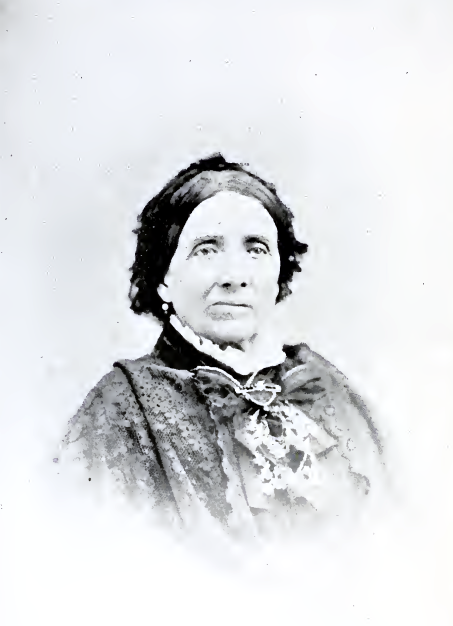
\includegraphics[scale=1]{../white/mrsWilliamAJudsonWhite.png}
	\caption {MRS. WILLIAM A. JUDSON}
\end{figure}





Henry,2 Henryi), married William B. Harrington. Child: 

water, Minn., and chaplain of the State Prison. 

Henry,2 Henryi), married Submit Rice, Nov. 10, 136. She 
was third daughter of Capt. Aaron Rice, who served in the War 
of 1812. She died at Fredonia, N. Y., Aug. 31, 1862, one 
month after the family arrived there, and Mr. Crane married 
second, Amelia Borden, second cousin to his first wife. He is a 
member of the East Ohio Conference of the M. E. Church. In 
and a law otflce, and was postmaster. Cliildren : 




He was by trade a shoemaker and born Jan. 28, 180-4. After 
trying several different locations their linal settlement was made 
in Bethlehem, Conn. Here Mr. Judson purchased a large farm, 
where for many years he, with the assistance of his sons, but 
principally of Francis E., carried on farming with considerable 
success, and became one of the most thrifty farmers of that 
region. During the latter years of his life, on account of failing 
health, was obliged to find a home with his children. He died 
Nov. 12, 1889. Mrs. Judson enjoyed a very strong constitution, 
and although it fell to her lot to labor as few women have done, 
in performing her allotted part of the duties upon a large dairy 
farm, yet she lived to enjoy a good old age ; and, had it not been 
for an accident which hastened her death, she would no doubt 
have remained much longer with her children, to whom she was 
fondly attached. She died July 11, 1885, at Trumbull, while 
stopping with her daughter Esther. She had been living a part 
of the time at her daughter's, Mrs. A. C. Peck, in Woodbury, 
and a part of the time at Trumbull. She had been a consistent 
member of the Church for over 50 years, and was 85 years and 
her kind ministrations in sickness, and her loving sympathy and 
words of encouragement in times of trouble. She had the mis- 
fortune to break her Iiip a few months before her death, and was 
never able to walk thereafter. Her remains were interred at 
Bethlehem, the funeral service having been lield in the Congrega- 
tional Church at that place. Children : 




resides in California. 


Wealthy A. Allen. 




Plumb B. Nichols. 


Peck. They reside in Woodbury, Conn., where Mr. J'cck is 
known as a successful business man and a skilful practitioner 
of dentistry. 





He, after teaching school at the age of 18, began as a clerk in 
a store at HotchkTssville, Conn., but caught the gold fever in 
ISJri) and made the trip to California, sailing round tlie Horn. 
The shining metal soon lost its charm for holding him in that 
locality, and he returned to Bethlehem, Conn., his home, by 
the way of the Nicaragua route. But while visiting a Spanish 
friend in Nicaragua, with whom he had made an acquaintance 
in California, heconceived the idea of constructing a sailing 
vessel in which to carry on a commercial and freighting trade 
with the natives about the lake there bearing that name. Soon 
after reaching home in the Spring of 1851 he began the build- 
ing of the vessel, and the Fall of that same year found him 
attempting to stem the current of the ri\\'er San Juan on his 
way to the lake. So many difficulties appeared that he sold 
his schooner for a nominal sum and entered the employ of the 
transportation company then carrying passengers to and from 
California to New York, engaging as fireman on one of the 
passenger boats running from (xraytown up the river and 
through the lake and return. So proficient did he become 
that he Avas soon promoted to the position of engineer, and 
from that to captain, and for several years was one of the 
most successful officers on the line, remaining with the com- 
pany until their charter was revoked and their property con- 
fiscated by that adventurer, William Walker, in the Spring of 
developing a desire to go West he purchased a farm in Elvas- 
ton, Hancock Co., HI., removed there and carried on farming 
a few years ; but at the solicitation of his brother Henry, then 
in Central America in the employ of a new company who had 
reopened the Nicaragua route, he, June 13, 1863, again sailed 
from New York for Gray town, where he arrived on the 23d, 
and immediately assumed his old position as captain on the 
line, continuing in that service until April 9, 1865, when from 
exposure and over-work he was stricken with a fever and d. 
at Graytown, Nicaragua, May 1. The body, although tem- 
porarily deposited in the United States naval burying-ground 
at Graytown, was finally brought home to Bethlehem, Conn., 
and placed in the cemetery there. He left tAvo children : 




residents of Placerville, Cal., for several years. Children all 
dead except the eldest one : 







hem, Conn., Feb. 1, 1855. He attended school in his native 
town and began as a clerk in a store, but when 20 years of 
age went to Nicaragua, at tlie solicitation of his brother, Le- 
Grand, for the purpose of entering the employ of the " Vander- 
bilt Transit Co." He began in the Fall of 1852 as fireman on 
one of their steamboats. It was not long before he was pro- 
moted to the position of engineer, and remained in the service 
of the company until their charter was annulled and their 




HKXHV 1'. .irnsoN. 




Mr. Judson then returned to Bethlehem, Coun., but soon pur- 
chased a farm in Elvaston, Hancock Co., 111., and removed to 
that place and carried on farming for a time, but it was not a 
business of his liking. A new company having been formed 
for reopening the Nicaragua line Mr. Judson was sought out 
and ejigaged to proceed to Graytown at the greatest p'ossible 
speed, important matters having been placed in his charge, 
requiring both promptness and secrecy, as the company's char- 
ter was at stake. He sailed from NeAV York Sept. 11, 1802, 
with drawings of an engine which was to be shipped, and 
designed for a boat then building at Graytown, and which must 
be completed on or before a certain date or the company's 
charter would be forfeited. Mr. Judson arrived at Aspinwall 
Sept. 21. There being no regular conveyance plying between 
there and Graytown, he chartered the schooner Susan Chase, 
and by canvassing the place found sutflcient freight for Gray- 
town to materially reduce his expenses in getting there, where 
he arrived Sept. 29, 10 P. M. The following day the steamer 
Granada was launched, and Mr. Judson began work assisting 
to get the boat ready to receive the machinery when it should 
steam was made and the Granada made her trial trip, saving 
the time limit by one day only. Mr. Judson was a natural 
mechanic, displaying remarkable skill. Beginning as a lire- 
man he was, Jan. 1, 1863, promoted to an engineer, and soon 
after to chief engineer of the whole line. His ability to 
accomplish the most difficult mechanical problems seemed to 
find no limit, although his preliminary training was exceed- 
ingly meagre. Late Thursday evening, April 27, 18Gr), while 
at Castillo, news came of the dangerous illness of his brother 
LeGrand at Graytown ; setting out at daylight in the morning 
he reached his brother's bedside at 3 o'clock V. M. the follow- 
ing day, to find him very low and rapidly sinking ; although 
everything was done that seemed possible, after watching over 
him constantly until 4 P. M., May 1, he passed away in quiet 
sleep. Mr. Judson remained in Nicaragua until April 3, 186(5, 
the company having relinquished the business. He reached 
New York ten days later and proceeded to Bethlehem, his 
native town, where he remained a few years Avorking on 
mechanical inventions, many of them proving of practical 
utility. About 1873 he removed to Boston, Mass., where his 
engineering skill gave him a position in the construction of 
the abattoir works at Brighton, where he again established a 
home, and at their completion he was rewarded with the situa- 
tion of chief engineer of the Avorks; a position which for a 
score of years he filled to the satisfaction of all concerned. 
During the last few years of his life Mr. Judson surtered from 
a disease of the kidney that finally terminated his life, 
although it became necessary, to prolong life, to remove 
one foot after the other, he attended regularly to his business, 
except while at the hospital, and kept up his usual cheerful 
and hopeful greeting to all, even to the last and fatal moment. 
He d. April 15, 1894, at Allston, a part of Brighton, where 
he last resided. An official of the corporation Avrote as fol- 
lows : "The recent decease of Henry P. Judson, engineer 
at the Brighton Abattoir, recalls to those conversant with the 
establishment of that institution his long and exceedingly 
able connection therewith. Coming to it at its inception as a 
stranger to its managers, he at once impressed them with his 
special fitness for the varied and, in many respects, peculiar 
demands of the situation ; and his long and faithful experience in its service has fully demonstrated the wisdom of his original selection. 

\begin{figure}[htp]
	\centering
	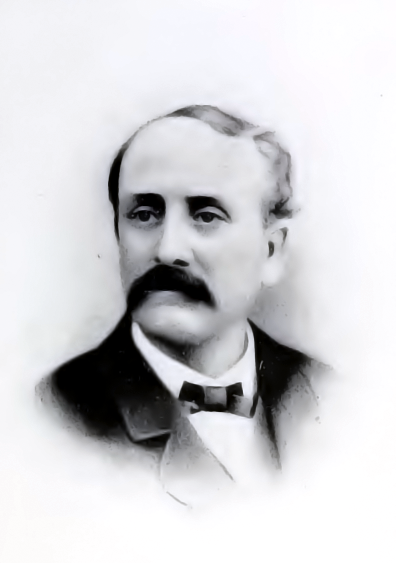
\includegraphics[scale=1]{../white/henryPJudsonWhite.png}
	\caption {HENRY P. JUDSON}
\end{figure}

"'To his thorough equipment as a practical engineer -was 
added a familiarity with the natural laws applicable to all 
branches of the business, and a further special faculty of 
being able to apply all such knowledge in the most economical 
manner to produce the best results. To the above combina- 
tion of qualities should also be added an absolute loyalty to 
what he conceived to be the best interests of the abattoir, 
and an utter disregard of his own comfort or convenience 
when they in any way conflicted with its requirements. To 
attempt to enumerate in detail his various services would be 
to practically give a history of the improved processes 
adopted during the last twenty years at the abattoir for the 
utilization of the various refuse products of the slaughtering 
business  an undertaking of altogether too great magnitude 
to be attempted in the present sketch, and we may perhaps 
conclude this imperfect notice with the reflection that the 
abattoir has been most fortunate in having for so long a 
period been able to have the services of one so exceptionally 
qualified and so thoroughly unselfish in his devotion to its 
interests." 

Mr. Judson had five cliildren, three d. young : 




1869, and settled in Trumbull, Conn., where Mr. Nichols car- 
ried on farming. She d. April 19, 1890. She was a person of 
rare womanly qualities. Although a great suflTerer for a long 
period before her death, she was always patient, hopeful, and 
even cheerful through it all, maintaining a perfect Christian 
faith to the very close of her life. She had three children, 
one, Louis, died in infancy. 



Silas,3 Heury,2 Heuryi), was Ijorn in Colebrook, N. H., April 7, 
with the family to Bethlehem, Conii., where upou a farm Robert 
grew to a youug man of seventeen years of age, passing the time 
in rendering what assistance he could about the farm work, and 
so constant were his services in demand that little time was allowed 
him for acquiring any education. In the year 1824 the family 
again returned to Colebrook, N. H., and resumed the work of 
clearing up a farm in that then wild country. As the health of the 
father soon became broken, his elder brother remaining in Con- 
necticut, Robert, although yet in his teens, was obliged to assume 
the entire responsibility of the work on the farm aiid care for the 
support and comfort of the family. By consummate energy and 
frugality of the strictest sort he managed to carry on the farm, 
and at the same time, by employing the son of a neighbor to look 
after his affairs at home during some of the Winter months, he 
improved the time in attending school at Lancaster, where, after 
spending two or three Winters and sawing wood and doing vari- 




ous chores in payment for his board, he graduated in 1831, and 
for several years afterward taught school Winters, keeping up 
the duties and responsibilities of a husbandman during the Hum- 
mer seasons. Feb. 25, 1836, he married Almira P.' daughter 
of Capt. John W. Bicknell, native of Barrington, R. I,, "born 
June 1, 1816. Mr. Bicknell for 30 years had been a seafaring 
man. In the year 1816 he removed to Canterbury, Conn., 
where he kept a hotel. After remaining here four years he 
removed to Canaan, Vt., a town lying near Colebrook. On 
Oct. 24, 1836, Mr. Crane left Colebrook to locate a home in the 
West. The Spring following found him at Beloit, Wis. Here 
he soon provided a shelter for his family, while they hastened to 
meet him, arriving there in August, 1837. Mr. Crane was one 
of the 16 original and active members known as the New England 
Emigrating Company that settled the town of Beloit, Wis. Here 
he resided until November, 1881, when to avoid the severe Win- 
ter seasons he removed to Micanopy, Fla., purchasing an orange 
grove, where he died Nov. 3, 1882, aged 75 years, 6 months and 
and an honest man. His wife, Almira, died at Beloit, Jan. 6, 
1854, aged 37 years and 7 months. Nov. 29, 1860, he married 
Jane A. French of Monroe, Conn. She died March 31, 1868, 
and he then married, March 25, 1869, Hephzibath J. Wilson, 
who survived him and resided in Florida until her death, April 
5, 1889. Had but one child : 

Henry, ' Heiiry'), married Elizabeth Rogers of Woodbury, Conn., 
Nov. 7, 1822, and settled in Bethlehem, Conn., where he died 
Aug. 10, 1867. She died there about the year 1887, leaving 
quite a little property to her children. Children : 






Silas, 3 Henry,2 Henryi), married 1st, Sarah S. Ayers, Jan. 19, 
1832; 2d, Laura Leach, Jan. 17, 1856. Had two children by 
first wife and one child by the second : 

and have a dan. 

Henry,- Henryi), married Sarah Atwood in Woodbury. Conn.. 
Nov. 11, 1829. Kept a tavern at Bethlehem Centre for several 




years. He died Dec. 9, 1836, aged 28 years, at Bethlehem, 
Conn. Child : 


Miss Harper; lived for a time in Waterbury, Conn., but 
later removed to Cheshire. 

Henry,2 Heuryi), married Gilman E. Hill, March 5, 1834. He 
was a native of Bethlehem, Conn., and resided there until the 
year 1854, when he removed to Middlebury, at which place he 
died. Deacon Hill was a man of influence, having been a mem- 
ber of the State legislature. Children : 



tion of Secretary of the Waterbury Brass Co. of Waterbury, 
Conn., where he resides and enjoys the esteem and confidence 
of his fellow-citizens. 

She was born in Stepney, Conn., April 15, 1821. Mr. Crane 
was a native of Bethlehem, Conn., and continued to reside there 

Children : \\\\



\begin{figure}[htp]
	\centering
	\includegraphics[scale=0.75]{../white/robertCraneMDWhite.png}
	\caption {ROBERT CRANE, MD}
\end{figure}

\begin{figure}[htp]
	\centering
	
\includegraphics[scale=0.75]{../white/robertCraneSignatureWhite.png}
	\caption {ROBERT CRANE'S SIGNATURE}
\end{figure}



ROBERT CRANE, MD Silas, =' Henry,2 Henryi), married Eunice M. Averill, Feb. 17, 
1847, at South Britain, Conn. She was born in Southbury, 
Conn., May 30, 1820. Mr. Crane took up the study of medicine, 
graduating from the Medical Department at Yale College in the 
year 1843. For several years he resided in Middlebury, Conn., 
where he practiced his profession ; was honored with the appoint- 
ment of postmaster, and was elected representative to the legisla- 
ture from that town. He afterward removed to Waterbury, 
Conn., where he became prominently associated in various kinds 
of business, including banking, manufacturing, etc. Here he 
was U. S. Assessor of Internal Revenue and member of the Com- 
mon Council. The activity and diligence with which he applied 
himself to all his undertakings, while it gave him financial suc- 
cess began seriously to wear upon his constitution. So apparent 
did it seem that a change of habits and responsibilities should be 
made that he removed to New Haven, where he might live more 
retired from active business strain and also have an opportunity 
to educate his sons, but even here he was drawn into serving his 
constituency in the City Council. He has a strong charactei" and 




an unswerving inclination to act riglitly in all matters, whetlier 
religious, social, or political. Children : 



22, 1870, while at Yale College. 

Heury,' Henryi), married Polly Allen, Sept. 4, 1.S44, and resided 
in Bethlehem, Conn. He died March 27, 1870. She died March 
28, 1876, aged 52 years. Children : 


Henry,2 Henryi), married Mary M. Amies, Nov. 12, 1833, at 
Westmoreland, N. Y. She was a native of Charlemont, Frank- 
lin Co., Mass., born Oct. 20, 110. Mr. Crane was born in 
Durham, 'liddlesex Co., Conn., and removed to New York State 
with his parents ; was a farmer and for many years resided in 
Westmoreland, where all his children were born. Late in life he 
removed to Silver Lake, Lincoln Co., South Dakota, where he 
died Nov. 20, 1878. Children : 


tute, Westmoreland, N. Y. 



Henryi), married Louisa Nash, April 7, 1833. She was a native 
of Denmark, N. Y., born Aug. 9, 1811. Mr. Crane died May 

27, 1871. She died Nov. 28, 'l893. Children : 




residence Lowville, N. Y. ; no children. 

N. Y. 

Henryi), married Susan C. Brown at New Haven, Conn., April 
23, 1844. She was a native of that place and born June -JC,, 




War of 1812, leaving the subject of this sketch, while but a year 
old, to be cared for aud reared by his Aunt Mehitable. He 
learned the trade of carriage-making aud for many years was 
engaged in that business in New Haven, Conn., where he died 
Nov. 19, 1888; and his wife April 29, 1889. Children: 

non, N. Y. 


A. Bond; residence. New Haven, Conn. 


Henryi), married, Oct. 5, 1840, Peter Bellinger, a native of 
Little Falls, Herldmer Co., N. Y., b. Feb. 19, 1803; by trade a 
tanner, aud settled first at Turin, N. Y. They afterwards 
removed to Denmark, N. Y., where she died Dec. 12, 1849, leav- 
ing two daughters. He enlisted as a private in Capt. P. W. 
Smith's Co.,'59th Reg., N. Y. S. V., in the Fall of 1861 ; taken 
sick and discharged in May, 1862, and died at Constable ville, 
Lewis Co., N. Y., July 16, 1862. Children: 


Fair child. 


Lyman; residence, Turin, N. Y. 


Hovey, and settled at Constableville, N. Y., where she d. 
Nov. 3, 1871, leaving one child. Mr. Hovey d. in the Winter 
of 1889. Child : 

N. Y. 

Henry, 2 Henry i), married John Wikoff and settled at Ontario, 
Knox Co., 111. Children: 






Henryi), married Hopkins. Child : 


Henry,2 Henryi), married Cornelia L. Whitmore. He is a farmer 
and resides (1880) at Ontario, 111. Children: 





Heury,2 Henryi), married J. M. Hitchcock; settled in Chicago, 



Henryi), married Reuben Hill of Manchester, N. Y., and resided 
on a farm about two miles from Clifton Springs, N. Y., where 
Mr. Hill died many years since. Mrs. Hill continued to reside 
on the same farm until her death about 1885. Children : 




b. and reared. 


Henry, ' Henryi), married Warner of Orleans, N. Y., and 

settled on a farm near Albion, Orleans Co., N. Y. Shortly prior 
to his death, which occurred Oct., 1878, he removed to the 
village of Albion, where he died. He was twice mamed but had 
no children by his second wife. Children : 



Petti ngill. 

Henryi), married John B. Crosby of Rush, Monroe Co., N. Y. 
He died about 1860, and his widow some ten years later. 

Children : 




Henryi), married Theodore Crosby of Canandaigua, N. Y., and 
a farmer. He was a brother of John B. who married her sister 
Polly. She died 1887 at Canandaigua, N. Y., leaving one 
daughter : 


Henryi), married Phebe Jane Howard of Dutchess Co., N. Y., 
and settled at Clifton Springs, N. Y. ; a farmer. He died in 
September, 1856, and his wife March 13, 1868, at Clifton Springs, 
N. Y. Children : 





Henryi), married Amy Clark, a native of Courtland, Courtlaud 
Co., N. Y. She was born in 1805. Mr. Crane was a farmer, 
and served during the War of 1812, having been stationed at 
Child : 


Henryi), married Rachel Berger. Lived at Adrian, Mich. He 
died Feb. 10, 1880, aged 85 years and 8 months ; buried at the 
old cemetery, Canandaigua, N. Y. Child : 


Henryi), married Reuben Beeman. Children: 


d. of consumption, Dec. 3, 1867, leaving three children : 





has three children : 





d. Aug. 12, 1883, leaving two children : 




and d. Aug. 9, 1892, leaving eight children : 













186G. Children : 






C. Albert Manning (Beeman) . 


Children : 




Henryi), married 1st, Eussell Colsou in 1823. He was drowned 
in 1825 ; left a daughter. Married 2d, Joshua Thompson in 
of 90 years old. Children : 









Nov., 1889; living on the old homestead, Canandalgua, N. Y. 





dence, Newark, N. Y. Children : 










Aug. 3, 1858, and died at San Diego, Cal., Feb. 11, 1893, leav- 
ing three children, residing at Denver, Colo. Children : 





of consumption at Denver, Colo., April 26, 1889, leaving: 


N. Y. 



Colo., March, 1877, where they reside. Children : 






Hatfield, Oct. 5, 1880; resides at Texarkana, Texas; is agent 
for the Pacific Express. Children : 




Heury,' Heury'), married Sarah Martin at Canandaioua, Ontario 
Co., N. Y., Feb. 6, 1846. She was born March 1;5, 1822. He 
is a farmer and resides at South Bristol. Has been a member of 
the New York State militia. Children : 



Henry, 2 Henryi), married Booth at Victor, N. Y., Dec, 



Henryi), married Margaret Davenport at Bristol, N. Y., Nov. 
11, 1S40. She was born in Monroe, Orange Co., N. Y., Jan. 
30, 1816. Occupation, farmer; residence, Fentonville, Genesee 
Co., Mich.; died Feb. 2, 1893. Children: 

1070-1. Jesse D., b. Oct. 2, 1841, at Canandaigua, N. Y. 

Henry, 2 Heury'), was born at Paterson, N. J. ; married at Lock- 
port, N. Y., June 3, 1855, Jeanette McKain. She was a native 
of Lockport, N. Y., and born Feb. 23, 1831. They removed 
to Amboy, 111., where their children were born. Subsequently the 
family removed to Chicago, 111., where Mr. Crane was for many 
years engaged in mercantile business. He died at Kirkwood, 
Mo., Aug. 17, 1880. Children: 

\begin{figure}[htp]
	\centering
	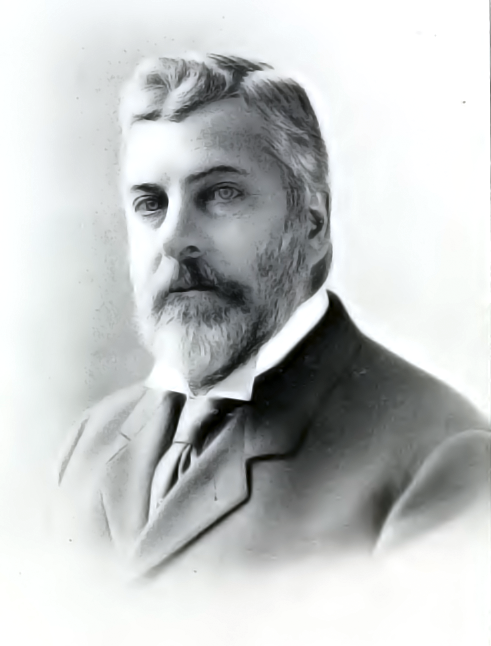
\includegraphics[scale=0.8]{../white/richardTellerCraneWhite.png}
	\caption {RICHARD TELLER CRANE}
\end{figure}

RICHARD TELLER CRANE Henry, 3 Henry,' Henryi), was born in Paterson, N. J., May 15, 
much to do with the better class of work in New York City and 
Paterson, N. J., during the first third of the nineteenth century 
and up to the time of the panic in 1837, when he was swept by 
the devastating tide and left in very straitened circumstances 
with a large family to provide for. The subject of this sketch, 
being next to the youngest of the children, was obliged to find a 
position in a factory when but nine years of age, and continued 
to work there until 1847, when he ohtained a situation to leani a 
trade in a brass foundry and tinishing shop in Brooklyn, X. \\ ., 
where he remained about four years. He afterwards secured 
employment in New York City, continuing there up to the year 
1855, when he removed to Chicago, 111., and laid the foundations 
for the establishment of the prosperous enterprises which are now 
known as the Crane Company and the Crane Elevator Company. 
The business was started in a very small way in the manufacture 
of brass castings, to which was gradually added the work of brass 
finishing in the steam-engine line. Afterwards was added the 
line of steam-fitters' supplies, the conducting of steam-heating 
business, the manufacture of wrought-iron pipe, steam-engine 
building, and finally the construction of steam and hydraulic 
elevators. In the development of business the two branches 
have been kept entirely separate, and the lines of each closely 
defined. The Crane Company now (1894) manufactures exclu- 
sively steam-fitters' supplies, that is, goods used for heating build- 
ings and steam-engineering work generally, while the other 
company is devoted entirely to the building of elevators. It is 
proper to state that both these institutions are the largest and 
best equipped in their line of any in the country, employing in 
normal times about 2,500 hands. The Crane Company, in addi- 
tion to running their factories, have branch stores in the fijllow- 
ing cities : New York, Philadelphia, St. Paul, Minneapolis, 
Duluth, Kansas City, Omaha, Los Angeles, San p>aucisco, Cal., 
and Portland, Oregon. Goods from both the above-named facto- 
ries are sold throughout the country, from the Atlantic to the 
Pacific. Very few instances can be found where business of a 
strictly competitive nature, not protected by patents or enjoying 
special privileges, has been conducted with such marked success. 

Notwithstanding the pressing demands on his time consequent 
to the conduct and development of such a gigantic enterprise, 
Mr. Crane has found opportunity for considering public questions, 
especially those of an educational nature, and no insignificant 
share of his time and means has been devoted to providing for 
the social and mental improvement of the lower classes, believing 
that in elevating the condition of that portion of our population 
he is helping to strengthen and perpetuate the principles of good 
government, the neglect of which may endanger the stability of 
our institutions, which have been the pride and joy of our prosper- 
ous country. The manual training school and kindergarten he 
believes to be a step in the right direction in furnishing a means 
by which the louver classes in society may be early helped to a 
self-sustaining position in the community where they live, thereby 
making them a support and not a menace to our highest and best 
Interests. 

So much in earnest was he on tliis subject that al)out the year 
Chicago to fit up an unused basement in the Tilden School, cor- 




ner of Lake aud Elizabeth Streets, for the purpose of trying 
manual training there. As the Board of Education were not 
inclined to supply anything beyond the empty basement, Mr. 
Crane began the work of putting it in order, and furnished it 
with 12 carpenters' benches fully equipped with proper tools, 
giving space for 24 lads to work at one time. In fact, has at his 
own expense furnished everything complete for systematic work, 
even to supplying a thoroughly competent teacher for three years, 
during which time this branch of the school has been enlarged by 
Mr. Crane obtaining another basement and fitting that, giving 
double the capacity of the first room. The manual training 
taught in the "Crane School" is now made compulsory. The 
boys from 11 to 15 years are taught, during certain hours each 
week, the proper use of tools and how to cultivate the eye and 
the hand in the manufacture of many useful articles. The Board 
of Education no longer look upon it as an experiment, but are 
now (1894) cooperating with Mr. Crane, and the same system 
has been introduced into some nine other schools in various parts 
of the city. Certainly great credit is due Mr. Crane for his gen- 
erosity and forethought in paving the way for the accomplishment 
of so much good, especially in the direction of helping the poor 
boys. 

He married, Oct. 8, 1857, Mary Josephine Prentice. She was 
born Feb. 22, 1836, and died Jan, 28, 1885. Children all born 
in Chicago, 111. : 


\begin{figure}[htp]
	\centering
	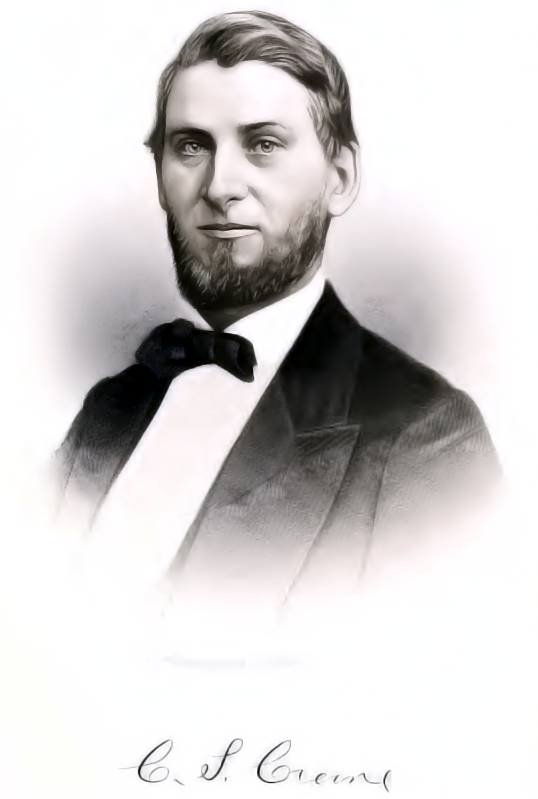
\includegraphics[scale=0.75]{../white/whitecharlesSquireCraneWhite.png}
	\caption {CHARLES SQUIRE CRANE}
\end{figure}



CHARLES S CRANE Henry,3 Henry,' Henryi), was born at Passaic Falls, Paterson, 
N. J., where he attended school during his boyhood days. At 
the age of 16 he went to Lockport, N. Y., to learn the trade of 
moulding. After which he returned to Paterson, aud for a time 
was engaged with the Danforth Locomotive Works as a moulder. 
In 1855 he removed to Chicago, 111., and entered into business 
with his brother in the manufacture of brass goods under the firm 
name of R. T. Crane \& Brother. In 1859 they added the foundry 
business, and in 1865 they introduced the manufacture of iron 
pipe, which they manufactured quite extensively, it being the 
first industry of the kind established west of Pittsburg, Penn. 
About the same time they added the manufacture of malleable 
iron. Soon after a stock company was formed and the business 
was conducted by the North Western Manufacturing Company, 
and was so continued until the year 1872, about which time Mr. 







-" U, \\£rj 



'-'->"v\_C 




Charles S. Crane retired from the company. In 1871 ]Mr. Crane 
assisted in organizing the Wright ct Lawther Oil and Lead iNIan- 
ufacturiug Company, accepting the otHce of vice-president, and 
in 1885 was chosen its president. Mr. Crane identified himself 
with various kinds of business and was always interested in 
public matters, whether of a local. State, or national character ; 
was widely known and highly respected. Sept. 23, 1857, he 
married Eliza J. Beyea of Paterson, N. J. He died Sept. -S, 
tou Boulevard, Chicago, 111. Children : 



Henry, 3 Henry, ' Henry'), married Harriet Carrier. He Avas a 
farmer and settled at Volney, Oswego Co., N. Y., where they 
died he April 24, 1878 ; she June 14, 1846. Children : 

resides at Volney; no children. 


Henryi), married. May 12, 1833, Samuel Emerson 3Iosher at 
Sauquoit, N. Y. Here they resided until March 25, 1.S41), after 
which time they removed to Ontario, 111., where she died ]March 
10, 1857. He died Feb. 23, 1867, at Galesburg, 111. They left 
the following children : 








rio, HI., Nov. 26, 1868. Children : 






Ontario, Ih., Sept. 19, 1867. Children: 












Henry," Henryi), married Jane E. Cook, Sept. 23, 1838, at Rus- 




sellburgli, Penn. She was a native of New Hartford, Oneida 
Co., N. Y., and born June 9, 1816. They resided in Paris, 
Oneida Co., N. Y. ; a farmer. He died May 9, 1872. Cliildren : 




Henryi), married Henry Gilbert of Gilbert's Mills, N. Y., in 
September, 1844, and died Nov. 30, 1855. Children: 







Henry, ' Henry, ' Henry'), married at Litchfield, Herkimer Co., 
N. Y., Sept. 5, 1852, Mary Grould Brown. She was a native of 
Litchfield, N. Y., and born Jan. 25, 1827. Mr. Crane was a 
native of Sauquoit, Oneida Co., N. Y., born Feb. 5, 1823 ; grad- 
uated from Dartmouth College 1849 ; read law with Hon. Joshua 
A. Spencer and Francis Kerman of Utica, N. Y., and began the 
practice of his profession in that city, continuing from 1852 to 
where he remained until Nov., 1863, when he removed to Leaven- 
worth, Kansas ; was County Attorney for two years, beginning 
January, 1864. He afterwards returned to Osawatomie, and was 
attorney for Miami County and also engaged in farming. Have 
an adopted daughter : 


Henry, 3 Henry,' Henryi), married Charles P. Adams, Aug. 10, 
1854, and settled at Randolph, N. Y., where he became engaged 
as a merchant. But for more than 20 years has been cashier of 
the State Bank of Randolph, where they now reside. Children : 


lives at .Jamestown, N. Y. ; have six children. He is an 
attorney at law. 


Henry,' Henryi), married Lizzie Johnson in 1860; settled at 
Troy, Ohio, and engaged in the grocery business. She died 
leaving a daughter. He died some years later. Children : 



New Mexico. He is general manager of the Pecos Valley 

Railroad. 



\section{SEVENTH GENERATION.}


Ebenezer,' John,- Henryi), marrk'd Ennice C. Rouer.s, May U, 
1832, at Tolland, Mass., and settled at West Granville, Hampden 
Co., Mass. He was a blacksmith by trade, but also carried on 
farming. Died at Goodrich, Mich., Oct. 17, 1850, aged 43 3'ears 
and 9 months. Children : 


ezer,3 John,' Henryi), married Sjdvester Stilman, ]\\Iarch 30, 


Amherst or Andover, Ohio. Child : 


Ebenezer,' John,- Henryi), married Roxauua P. Lyon, Oct. 19, 
Hartland, Conn., then removed to Winsted, Conn., wliere he 
died May 14, 1854. Children : 






Ebenezer,' Johu,' Henryi), married William Cowdry, Jan. 11, 
1835; settled at Granville, ]Mass., but after'vards removed to 
Ohio, where their son Lester D. was born. Children : 





Ebeuezer,3 John,- Henry'), married Sarah Parker. Sht- was a 
native of Wolcott, Conn., born in February. 1.S15, and dieil 
May 27, 1872, at Burlington, Conn., where the family resideil. 




Mr. Crane was a farmer aud also died at Burliugtou, Conn., Aug. 
19, 1881. Children: 

ezer,3 John,2 Henryi), married Ansel Pratt, Dec. 16, 1855; set- 
tled in Burlington, Conn. Had but one child : 


Mr. Crane settled first in Burlington, but after a few years 
removed to Meriden, and later on to Naugatuck. His occupation 
was the making of knife blades. Children : 


Ebenezer,3 john,' Henryi), married Francis J. Rathbun, April 
17, 1850, at Waterbury, Conn. Lived for a short time in Hart- 
land, but mainly their home has been iu Burlington ; now resides 
at Bristol. Children : 







Ebenezer,3 John,' Henryi), married Jerusha Stoddard, February, 
1838, at Monroe, Mich., where he resided some years and where 
his children were born. He afterwards removed to Penn Yan, 
where he carried on the business of a carpenter and contractor. 

Children : 



1127- 




Frank D. 


1128- 




Mary L. 


1129- 




Delos S. 


1130- 




Charles Z. 


1131- 




Anna G. 


1132- 




Henry W. 


1133- 




Katie G. 


1184- 




Russell A. 



Ebenezer,3 John,' Henry'), married William D. Washburn, July 
4, 1840, at Jerusalem, Yates Co., N. Y. He was born at Fort 
Plains, Montgomery Co., N. Y. Their residence for a time was 
at Jerusalem, where their two eldest children were born, after 
which they removed to Italy Hill, Yates Co., N. Y., where their 
daughter Annie was born. From there they removed to Pultney, 
Steuben Co., N. Y., where P'lorence and Melissa were boria. 
But January, 1<S55, found the family in the town of Wayne. 
Mr. Washburn was a tailor by trade. Children : 




\begin{figure}[htp]
	\centering
	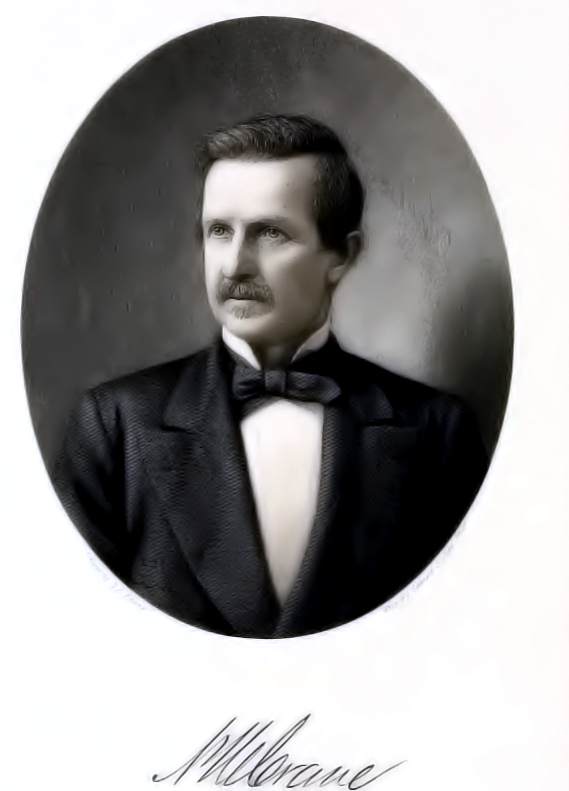
\includegraphics[scale=0.75]{../white/niromSCraneWhite.png}
	\caption {GEN. NIROM MARIUM CRANE}
\end{figure}

GEN. NIROM MARIUM CRANE (Nirom, Daniel,' Ebenezer,' John, 2 Henryi), born at Penu Yau, Yates 
Co., N. Y.,.Dec. 13, 1828. His father, a well-to-do farmer, 
assisted him to a liberal education, and being possessed of no 
small degree of ambition, as well as a desire to gain a position 
among his colaborers in life, he, in his seventeenth year, left the old 
homestead and went to the neighboring town of Wayne, Steuben 
Co., N. Y., to occupy a situation as clerk in a store for Harry 
Easton. Here he remained about two years and then returned to 
Penn Yan to accept a similar position in the employ of Hancock 
\& McNulty. In the Spring of 1849 he began business for him- 
self, opening a store for the sale of general merchandise in the 
town where he first began his clerkship, Wayne. Oct. 19, 1852, 
he was married there to Marie Louise, youngest daughter of 
Mathew McDowell, an accomplished lady, graduate of Alfred 
Seminary. April, 1853, he removed to Ilornellsville, N. Y., 
where he continued in the dry goods ti-ade until the year 1856, at 
which time the first banking establishment was opened in the 
town, the "Bank of Hornellsville," and Mr. Crane was chosen 
Vice-President. The following year, 1857, he was honored fur- 
the bank closed its business and Mr. Crane opened a private 
banking office and continued the business until the breaking out 
of the Rebellion. Already the patriotic blood which had been 
instilled into the very organization and conduct of the subject 
of this sketch had asserted itself, and was only awaiting an oppor- 
tunity when his public spirit and devotion to country should more 
prominently be made known. He descended through :i Hue of 
ancestors who could and did show their courage in times of need. 
Captain Henry, his progenitor, experienced more than 35 years 
of civil and military life. Captain John, who died in New York 
on his return from an expedition to Canada, left an enviable 
career as a statesman and soldier. Daniel, the grandfather of 
Gen. Nirom, gave four years of service diu-ing tlu' w:ir of the 
Revolution, so that in some measure it may l>e said that he 
partook of a soldierly make-up. He early enlisteil in the New 




York State militia aud for some years was iu eommaucl of the 
Canacadea Light Guards, one of the best companies of the 
National Guard of the State, but April 12, 1861, the attack 
on Fort Sumter found him Lieut. -Colonel of the 60th Regiment 
New York militia, and one of the first to raise a company for 
the war, aud joining the twenty-third (Southern tier) Reg. N. 
Y. State Volunteers, was chosen Lieiit.-Colonel. He was in 
command of this regiment, which was a division of the 1st 
Army Corps, from 1861 to 1863, and joined in the engage- 
ments at Rappahannock, Sulphur Springs, Grove ton, the Second 
Bull Run, Chantilly, South Mountain and Antietam. After the 
last named battle he was in 1862 appointed Acting Inspector- 
General of First Army Corps on Staff of Major-General John F. 
Reynolds, where he served until after the battle of Fredericks- 
burg. At the last named battle he acted as Aide-de-Camp to 
General Reynolds on the field, and was complimented in general 
orders for gallant services during action. Being superseded as 
Inspector-General by Col. Bankhead of the regular army, Gen. 
Crane was appointed in 1863 Assistant Provost Marshal General 
of the Army of the Potomac on Staff of General Hooker, and con- 
tinued iu that position until made Colonel of the 107th Reg. N. 
Y. Vols. ; was at Gettysburg in command of a regiment. In the 
Fall of 1863 went to join General Sherman with the 20th Army 
Corps ; was in the Atlanta campaign aud in command of a brigade 
at the capture of the last named city, and marched with Sherman 
through the Carolinas ; was present at the surrender of Gen. 
Johnston's army near Raleigh, N. C. ; took part in battles of 
Averasboro and Bentonville ; was brevetted Brigadier-General on 
March 19, 1865, for gallant and meritorious services rendered 
during the campaign through Georgia and the Carolinas. The 
war having been brought to a close. Gen. Crane received his dis- 
charge from the army in Juue, 1865, having experienced four 
years and two months active service in the field. One of his 
associates in the 107th Reg., N. Y. Vols., in sketching the services 
of that regiment, says : "In Colonel Crane it had a commander 
who was an accomplished military man and one always ready to 
lead where need required. His abilities as an ofiScer were quickly 
recognized at brigade, division, and corps headquarters, and it 
followed that he was assigned with his regiment to many impor- 
tant and responsible duties. He was much beloved and admired 
by his men, aud the 'Little Colouel,' as the boys used to call 
him, made a record of which they were justly proud." 

Soon after returning to his home in Hornellsville he established 
in the Fall of 1865 another banking estabhshmeut, and the same 
has for many years been known as "Crane's Bank," and of 
which he is President, and his son, Sidney Hallett Crane, Cashier. 
In November, 1868, Gen. Crane was elected Clerk for Steuben 
County to serve for three years. He was appointed by Gov. 
Robinsou, and confirmed by the Senate of New York, one of the 




first Trustees of the Soldiers aud Sailors' Home at Bath, and at a 
meeting of the board elected Treasurer for two years. He pnn-ed 
a very active and etticient worker, ever striving to make the institu- 
tion a means of comfort to those so unfortunate as to require aid 
at its doors. As a business man Gen. Crane ranks high among 
his fellow's. For many years he has been a member of " Christ 
Church" at Hornellsville, also serving as vestryman, and is 
greatly esteemed as a citizen. At a meeting of some of the 
descendants of the Crane Family, held at New Haven, Conn., 
Sept. 8, 1880, the Crane Genealogical Association was formed 
for the purpose of encouraging genealogical work among mem- 
bers of the family, and Gen. Crane was chosen first Vice-Presi- 
dent. At a subsequent meeting of this Association, held at 
Chickering Hall, New York City, he was present, and while pre- 
siding made a very graceful speech, in which he expressed his 
thorough interest in the history of the family. Children : 


Daniel, 4 Ebenezer,' John, ' Henry'), married Almira Randall and 
settled in Jerusalem, Yates Co., N. Y. ; a farmer. Children: 


11-12-2. William S., b. Dec. 14, 1843; residence in Detroit, JNlicb., 







Ebenezer,' John, ' Henryi), married Ann Merrill in 1848. She 
was born Dec. 11, 1830, and died July 26, 185o. Mr. Crane 
died at Ypsilauti, Mich., Oct. 25, 1878. Children: 

114<,) 1. Mortimer 11., b. Nov. 25, 1849; m. Jan., 1884, Lottie, dau. 
of Alvin and Margaret Mead; resides at Ypsilanti, Mich. 

Ebenezer,3 John,2 Henryi), married Dorcas E. WIuh'Ut at lU'ii- 
tou, Yates Co., N. Y., June 5, 1849. She was l)()ni in Yates 
Co., Feb. 15, 1831. Mr. Crane settled in Benton: a pliysieian 
and graduate of Geneva Medical College in 18 IC; has held the 
office of Supervisor and Superintendent of Schools. .Airs. Crane 
died May 13, 1877. Child : 


Ebenezer,' Jolai,- Henrv'), married at .Ierus:deni. Yates Co.. N. 




Y., Lucy P. Benedict, Nov. 5, 1840, and for a brief time resided 
at Italy, Yates Co., N. Y., and also in Jerusalem, but removed 
to Somerset, Mich., before 1852; subsequently lived in Addison, 
Mich. Children : 





E])enezer,3 John,' Henry'), born in Clinton, Conn.; married 
George Redfield Burrows, Nov. 25, 1838. He was also a native 
of CUnton, where they settled; was born Oct. 29, 1815, son of 
John and Jeunette Redfield Burrows. Occupation, a mariner, 
and has for many years been in the employ of the N. Y. \& H. 
Steamboat Co. Children : 


Bushuell, Feb. 14, 1866; served in the U. S. Navy and Haytian 
Navy. 



1873, Austin Lord, a physician. North Haven, Conn. 


Ebeuezer,3 John,' Henry'), born in Clinton, Conn., and died 
there ; married Ely Stannard, by whom she had one child. After 
the death of Mr. Stannard she married Jared Hurd. She died 
Dec. 27, 1866. Her children : 




Daniel,' Ebenezer,' John,' Henry'), married D. S. Dibbell of 
Baltimore, Md., Dec. 13, 1865. Children: 


City. 


Ebenezer," John,' Henry'), married Elizabeth Tuthil, and for 
some years resided at 222 Spring Street, New York City. He 
died about 1891. Children : 




Ebeuezer,3 John,' Henry'), married Mary S. Willard, Oct. 18, 
1848, at Clinton, Conn. He was a tea merchant in New York 




City, one of the firm of George W. Lane \& Co. of Front Street, 
and died in Saybrook, Conn., Oct. 4, 1875. A man greatly 
respected for bis courteous manners and unswerving integrity. 
For a quarter of a century be was connected witli tbe above pop- 
ular firm, and no merchant stood higher among his associates 
than he. Children : 




L. Nichols, Bridgeport, Conn. 

Augusta Storn of New Yorlt. 

Ebeiiezer,3 John,' Henryi), born in Baltimore, Md., where he 
was married, July 3, 1863, to Ellen Gaines D. Cormis. She was 
born in Norfolk, Va., Fel). 3, 1845. Mr. Crane was educated 
at St. Mary's College, Baltimore. About 1871 he removed to 
New York City, where he engaged in the silk goods trade. 

Children : 








Nathaniel, 3 Theophilus,' Henryi), married Thomas A. Stevens, 
a native of Killingworth, Conn., Dec. 25, 1838, at Madison, 
Conn. He was a carriage-maker; removed to Birmingham, 
Mich., and from there to Port Huron, Mich., where he died 
March 23, 1857. She died there Jan. 14, 1887. Children : 






Mich., July 13, 1867, and had: 








Nathaniel, 3 Theophilus,- Heury'), married Elsworth Scrantou. 
Children : 










Elisha,'* Natliauiel,' Theophilus,' Heury'), married Alleu, 

1857, and died June 15, 1873, leaving one child: 


Nathaniel, 3 Theophilus, 2 Heury'), married Noble Blatchley, 18G4. 

Oue child : 

iel, ' Theophilus,' Henryi), married William Golden, 1870. Has 
one child. 

Nathaniel,' Theophilus,' Heuryi), was born in Kent, Ohio, and 
married Abby Eliza Melleu, a native of Quincy, 111., Jan. 2, 
and served until the close of the war; on staft" duty, A. D. C, 
3d Brig., 1st Div., 15th Army Corps; was wounded at battle of 
Missionary Ridge, Ga. ; settled at Mt. Pleasant, Iowa ; a hard- 
ware merchant; and here he died Dec. 20, 1887. Children: 



1185- 




Anna Mabel. 


1186- 




Herbert Wilder. 


1187- 




Laura Evelyn. 


1188- 




Fred Baron. 


1189- 




George Eber. 


1190- 




Julius Howard. 


1191- 




Ralph Knowlton. 


1192- 




Helen Van Doorn. 



iel, ' Theophilus,' Henryi), married Louisa M. Dickerman at 
Middlebury, Vt., Oct. 20, 1831. They resided for a time in 
Vermont and then removed West. Two or three children not 
named here died young, before the family left Vermont. 

Children : 





Martha Jane. 




Maria Ann. 




John Edgar. 




Ezra. 


1198-5. 


James. 




Demis. 


1200-7. 


Eva. 



Nathaniel, 3 Theophilus,' Henryi), married James T. Foster, 




Jan. 20, 1836, and first settled iu Middlel)ury, Vt., soon removed 
from there and was last residing in Astoria, N. Y. Children : 









Nathauiel,3 Theophilns, 2 Henryi), married 1st, Leonard G. Lester 
of Port Jervis, N. Y., Sept. 27, 1849. He was killed June 20, 
1864, at battle of Kenesaw Mountain, Ga. She married 2d, 
April 11, 1872, J. W. Fields, by whom she had no children. 

Child : 


Nathaniel, 3 Theophilus, 2 Henryi), married April 19, 1841, p:iiza 
B. Corlew ; settled in Middlebury, Vt. ; a farmer, and removed 
to Sadorus, 111., where he died April 17, 1880. Children: 


18G1, and served nntil his death, May IG, 18()4. 


Nathaniel,"' Theophilus,' Henry'), married R. .]. 'Melius at East 
Greenbush, N. Y., Sept. 23, 1858. Afterwards removed to Bath 
on the Hudson, where he entered the grocery business. Children : 






Nathaniel, 3 Theoplulus,' Henry'), was born at Stockton. Chau- 
tauqua Co., N. Y. Went with his parents to the town of Leroy, 
Ohio, about the year 1827. When a young man the family 
removed to Indiana and took up a residence near South Bend. 
He was a farmer, and married Nancy Keep. His hist icsiih'ucc 
was at Hamilton, Steuben Co., Ind. He was killed by :i hull 
some years ago. Children : 









Nathaniel, 3 Tlieophilus,' Henryi), was bom in Stockton, Chau- 
tauqua Co., N. Y. ; married, Feb. 23, 1842, Aurilla Ferris, at 
Jackson, Mich. He removed from there to Ridgeville, 111., and 
For 21 years Mr. Crain followed the occupation of a mariner, 
rising in due time from cabin-boy, at the age of 13, through all 
the stages of rank to master of the vessel ; sailing ten years on 
the lakes. In 1849 he crossed the plains to California, but 
returned in 1853, since which time he has followed farming. 

Children : 













1227-11. Ida May, b. Dec. 30, 1863, at Durand, Wis. 



Nathaniel, 3 Theophilus,' Henryi), married Olivia Hill about 
1844, at Evanston, 111. She died about the year 1873, and he 
married Mrs. Siter, whose maiden name was Dama L. Morse. 
No children by either marriage. Was a cooper by trade and car- 
ried on that business. Was also engaged in the real estate trade 
for some years at Evanston. After the death of his sister, Mrs. 
Kelley, he adopted two of her children : 



Nathaniel, 3 Theophilus,' Henryi), married Alonzo Burroughs at 
Evanston, 111. He was formerly from Ashtabula, Ohio, and 
moved from that locality in the year 1842, in company with his 
two sisters, making their journey in a "Prairie Schooner," as 
those large covered wagons were called in which families per- 
formed their migrations when in pursuit of a location for a home 
at the then far West. Children : 










Nathaniel,' Tlieophilus,' Heuryi), was born in Stockton, Chau- 
tauqua Co., N. Y. In 1833 his parents removed to Le Roy, Oliio, 
and from there they removed in 1836 to De Kalb Co., Ind. In 
1840, at the age of 18, Mr. Craiu went to Dutcliman's Point, now 
Glenwood, near Northfield, 111., to work for his cousin John Miller. 
After a brief time he returned to his home in Indiana, where he 
remained until his mother's death in 1842, when he located in the 
known as Evanston, 111., and entered the employ of William 
Foster to learn the trade of a cooper, and for six years carried 
on the cooperage business. But in the Spring of 1850 he " caught 
the gold fever," and in company with his brother Osro and some 
of his neighbors, started overland for California. They made a 
very quick trip of it and were styled the "Lightning Express." 
Their first mining venture was in a place called in honor of the 
party "Greenhorn Caiion," and has since retained that name. 
Grain's Gulch, also named for them, still goes by that name. 
Charles Grain returned home in March, 1851, and engaged in 
market gardening, continuing in that business until 1875, when 
he became a dealer in real estate. He married in 1846 Sarah 
Burroughs, formerly from Ashtabula, Ohio, sister of Alonzo 
Burroughs, who married Anna L. Grain. Mr. Grain died June 
2, 1891. Children: 












Nathaniel, 3 Theophilus,' Henryi) . She early in life went to what 
is now called Evanston, 111., where her brothers then resided, and 
for about eight years was emjJoyed in Chicago, 111. She married 
Daniel B. Kelley, and some eight years later died leaving three 
daughters. Mr. Kelley died the following year. Children : 



Iowa. 


Nathaniel, 3 Theophilus,' Ilenryi). Before her marriage sjie 
passed several years with her brother Osro in what is now 
Evanston, 111. Soon after her return to Indiana, where her father 




then resided, she married Russell Little and settled on a farm not 
far from her father's home. Had ten children. The names of 
only four have been obtained : 





Nathaniel, 3 Theophilus,' Henry'), married Edward Haydon 
Morton, Oct. 19, 1852, and had one child. Post-Offlce address, 
Middleton, Vt. 


Nathaniel, 3 Theophilus,' Henryi), was born at Malone, N. Y. ; 
married, Oct. 24, 1848, at Yonge, Ont., Mary Shipman, a native 
of that place. Settled at Ogxlensburg, N. Y. ; cabinetmaker by 
trade. Children : 

June 29, 1886 ; resides at New Haven, Conn. ; no children. 

Ezra,4 Nathaniel,' Theophilus,' Henryi), married, March 8, 1858, 
Amasa Sawyer Tracy, a native of Dover, Me., born March 16, 








Nathaniel,3Theophilus, 2 Henryi), married Andrew J. Crain [856]. 
He was born in Stockton, N. Y., in 1826; was son of Charles 
and Fidelia (Case) Crain. (See page 114.) For a time resided 
at Eau Goalie, Dunn Co., Wis. ; late residence, Farm Hill, Pierce 
Co., Wis. Children: 





Nathaniel, 3 Theophilus,' Henryi), married, November, 1867, 
Widow Holland, whose maiden name was Ruth Lavinnia Bi-isfo-s, 




she having one son by her first husband. They settled in St. 
Charles, Minn. In June, 1872, they removed to New Mexico, 
where Mr. Crane died July, 1876. December followino-, the 
widow and children returned to Minnesota, and have made thcii' 
home at Winona. Children : 





Ezra,' Nathaniel,' Theophilus,- Henryi), married Esther L. 
Portis at Cleveland, Ohio. She was a native of Thorn Hill, 
Scotland. He enlisted in the Ohio Vol. Infantry, 7th Reg. ; was 
captain, and promoted to major and colonel of the same regiment ; 
a very brave soldier. He was killed at the battle of Renggold, 
Dec. 27, 1863. Children : 

12G3  1. William Cook, b. .Jan. 20, 1858; m. Miss Axworthy; no 

children. 
12(U 2. James Robert, b. June 7, 1800; m. Catherine Wedell ; no 

children. 

LsOl ; no children. 

Ezra,"* Nathaniel,-' Theophilus,' Henryi), married Viola L. Lake, 
April 27, I860.- She was a native of Denmark, Lewis Co., N. 
Y., born March 28, 1844. Mr. Crane has lived in Rensselaer 
Falls, N. Y., and held the office of deputy sheriff and constable 
for 32 years. Children : 


NathanieU' Theophilus,' Henryi), was a mitive of Stockton, 
Chautnu(iua Co., N. Y. Removed Avith his parents to Spring 
Valley, Minn., where he married Nellie S. Thayer. Oct. 20. l.SCxS. 
Nov. 7, 1894, he was residing at Fargo, N. Dak. Cliildri-n : 



Nathaniel,-' Theophilus,- Henry'), married 1st, Flora A. Church, 
wlio died in 187;'); mai'ried 2(1, Amanda Learned. She dii'd in 
1.S.S7, leaving a son Callie or Calvin. He in 1.S91 married .'L'Iis 
IJronson. Mr. Crane enlisted, April 16, 1861, for the late war as 
private, and was discharged Oct. 29, 1865, as First Lieut., Co. K, 




7th Kansas Cav. At the close of the war he went to Nebraska, 
and since 1867 has made his home in Ashland. Child : 

Nathaniel,:* Theophilus,' Henryi) , married, in 1867, James Tyler ; 
reside in Lincoln, Neb. Children : 





Nathaniel, 3 Theophilus,' Henry'), married E. B. Woodbury in 



Nathaniel, 3 Theophilus,' Henryi), married Delia Curtiss at 
In early life Mr. Crane followed the millwright business, but 
enlisted in 1862 to serve in the war with the 68th Ohio Vols. 
Late residence, Paw Paw, Van Buren Co., Mich. Children, born 
in Ravenna : 

dence, Muskegon, Mich., where he is a practicing physi- 
cian. 


Nathaniel,' Theophilus,' Henry'), married Margaret Bradley of 
Camden, Mich., July 4, 1858. Had one child : 


Nathaniel,' Theophilus,' Henryi), married Ester Bradley of 
Camden, Mich., Dee. 24, 1863, and settled in that place, where 
he died Feb. 16, 1872, leaving an only daughter: 


iel,2 Theophilus,' Henry'), was born in Canton, St. Lawrence 
Co., N. Y. ; married, March 27, 1851, Fidelia Brainard, a native 
of Gustavus, Trumbull Co., Ohio, where they reside. He fol- 
lows the occupation of a steamboat pilot. Children : 





Nathaniel, 3 Theopbilus,' Henryi), married, Aug. 12, 1851, Jane 
Eliza Bunker, a native of New York City, and born April 2fi, 
Mr. Crane being in feeble health, returned to New York City, 
where he died in April, 1890. Children : 



Sing Sing, N. Y. 
1297-10. Charles Bunker, b. April 24, 1874, in Yonkers, N. Y. 

Nathaniel, 3 Theophilus,' Henryi), born at Rondout, N. Y. ; 
married, Feb. 11, 1858, at Silver Hill, N. C, Jannette p:iizabeth 
Residence at present (1894) at Corinth, N. Y. Children: 

1299-1. Jane Eliza, b. Aug. 5, 1860, at Silver Hill, N. C. 










Ezra,' Nathaniel, 3 Theophilus,' Henryi), married M. F. Rowe, 
Yonkers, N. Y. ; removed to Sing Sing, N. Y., where Mr. Rowe 
and his son are proprietors of a newspaper. Children : 



Nathaniel, 3 Theophilus,' Henryi), married, in 1.S67, William 
Harkisheimer, a native of New York City, born 1847, and 
removed to Jacksonville, Fla. Children : 




Ezra,4 Nathaniel, 3 Theophilus,- Henryi), married, Oct. 13, 1SG9, 




at Burlington, Vt., Margaret Hood Hill, a native of Nashua, N. 
H., born Dec. 11, 1850. He was born at Cambridge, Vt. ; en- 
listed as a soldier in the late war, serving in Virginia during Win- 
ter of 1862 and 1863. Settled for a time at Burlington, Vt., but 
in 1894 was residing at St. Albans, Vt. ; an express agent. 
Children : 


store. 

Robert Gr.,' Silas, ' Henry,' Henryi), married Dora Wakefield, 
daughter of Elder Edwin W. Conley, March 4, 1873. Children : 

\begin{figure}[htp]
	\centering
	\includegraphics[scale=0.75]{../white/EBCraneWhite.png}
	\caption {ELLERY BICKNELL CRANE}
\end{figure}

\begin{figure}[htp]
	\centering
	
\includegraphics[scale=0.75]{../white/EBCraneSigWhite.png}
	\caption {ELLERY BICKNELL CRANE'S SIGNATURE}
\end{figure}


ELLERY B CRANE (Robert P., Eleazer, Robert G.,' Silas, ' Henry,' Henry'), born at Colebrook, Coos 
Co., N. H., Nov. 12, 1836; married Salona Aldrich Rawson, 
May 13, 1859, at the home of his uncle, Samuel B. Cooper, 
Esq., in Beloit, Rock Co., Wis., Rev. C. P. Bush performing 
the ceremony. In the Summer of 1837, his mother, in com- 
pany with her brother, George W. Bicknell, Eleazer Crane and 
his wife, grandfather and grandmother of the subject of this 
sketch, together with his aunt, Sarah T. Crane, set out from the 
town of Colebrook for their new western home, which the father, 
Robert P. Crane, had already gone to establish. A private team 
carried them to Burlington, Vt., where they took a steamboat for 
Whitehall, N. Y. ; thence by canal via Troy to Buffalo, N. Y. ; 
again patronizing the steamboat to Detroit, Mich. ; thence by 
team to Pittsfield, Mich., where a short stop was made at the 
home of an uncle Prudden. After a few weeks' delay the journey 
was again taken up, the mother travelling the remaining distance 
to Beloit, Rock Co., Wis., in a lumber wagon drawn by four 
horses driven by Capt. Thomas Crosby. The party from Pitts- 
field to Beloit consisted of the mother, Mrs. R. P. Crane, and 
baby (Ellery), Thomas Crosby, his wife and baby (George), Mr. 
Crosby's mother, and Mrs. James Cass, all from Colebrook, N. 
H. They arrived at their destination August 9, thoroughly ex- 
hausted from the trials of the journey, and on that day Ellery 
Bicknell Crane was lacking three days of being nine months old. 
In this then new western town Mr. Crane was reared, receiving 
his education in the schools there, both common and select, and 
was a pupil at the seminary when it was transferred from the 
basement of the Congregational Church to the first Beloit College 

In the year 1860 Mr. Crane made the trip overland to Cali- 
fornia with private team. After si)ending little more than two 
years in California and Oregon he returned via the Isthmus to 




New York City, intending to proceed to his old liome at Beloit, 
Wis., but was persuaded by friends of his Avife to locate in 
Boston, Mass., where he remained little more than four years, as 
salesman and bookkeeper for a lumber merchant. lii Ai)ril, 
1867, he removed to Worcester, where he located a lumber-yard 
and established himself in that business, and now (l.S'J5) after 
of his adoption, and where he has enjoyed the confidence of his 
fellow-citizens in so far as having been elected to represent his 
ward both in the Council and Aldermauic chamber for a term of 
years, and recently elected to rei)resent the 21st District (his 
ward) in the Massachusetts Legislature. For 12 years he was 
President of the Worcester Society of Antiquity ; has been a 
member of the Board of Trustees of the Worcester County 
Mechanics Association for several years, its Vice-President two 
years and President two terms ; a member of the Board of 
Directors of the Worcester Board of Trade and one of its Vice- 
Presidents. Mr. Crane has always been an active, public-spirited 
citizen, ever ready to contribute a portion of his time to the 
service of the public weal. For several years he was President 
of the Builders' Exchange, also one of the founders of the associa- 
tion known as the Sons and Daughters of New Hampshire and 
for three years its President. He compiled and published in 
deeply interested in matters of local history and family genealogy. 

Child : 


Silas, 3 Henry, ' Heury'), married Ralph Muuson ; settled in Beth- 
lehem, Conn., and had three children. He died Nov. 2;), 18'.M, 
in the 71st year of his age. Children : 




lol9. Charles S. Crane- [98.S], (.lohu X.,'- Phiiieas,'"' 
Robert CI.,** Silas, ' Henry,- Henry'), married Imogene .7. MoitIs 
('f Woodbury, Conn., Feb. IG, 1847, and for a short time lived in 
that place. About 1856 removed to Monroe, Conn. ; subsecinently 
he removed to Breckenridge, Mo., but in 1894 was residing in 
Proctorville, Mo. Children : 


in Chicago, III. ; no children. 





G.,4 Silas, 3 Henry,2 Henryi), married Cornelia Serry, Nov. 18, 


Robert G.,' Silas, ' Heury,' Henryi), married Gilbert Allen, 
March 11, 1852, in Bethlehem, Conn. Children: 






G.,' Silas, 3 Henry,2 Henry'), married Francis E. Judson [979] 
at Bethlehem, Conn., April 29, 1873. He for many years was 
engaged in business there as a merchant, but failing in health was 
obliged to retire from active trade, and for the past few years 
has resided in Allston and Cambridgeport, Mass., assisting and 
caring for his brother Henry during his entire sickness. Since 
whose death he has removed to Woodbury, Conn. Have one 
child : 


G.,' Silas, 3 Henry,2 Henryi), married Levi T. Knox, Nov. 2, 
1854, and settled at Bethlehem, Conn. Child : 


Robert G.,"* Silas, ' Henry,' Heiiryi), married David B. Jackson, 
Oct. 26, 1864. Children : 




Robert G.,'* Silas, ' Henry, ' Henry'), married Sarah Jane Stone, 
April 18, 1864; resided for a time in Bethlehem, Conn., after- 
ward removed to Morris, Conn. Now (1894) living iu Bay City, 
Mich. ; was a soldier in the late war. Children : 


Robert G.,'* Silas, ' Henry,' Henry'), married Frances Hoyt at 
Bethlehem, Conn., Jan. 5, 1878. She was a native of Warren, 




Conn., bom June 4, 1856. He was a painter and settled in his 
native town, Betlilehem, Conn. Children : 






Robert G.," Silas, ' Henry, ' Henry'), married Cordelia I. Corl'ett 
of New Haven, Conn., Aug. 28, 1888. Dr. Crane was l)()rn in 
Waterbury, Conn. ; a graduate from Yale Academic Dei)artnu'nt 
in 1885, and in 1887 from the Medical Department of Yale Tiii- 
versity. He served on the House Staff of the New Haven Hospi- 
tal about a year and a half, when his ability as a physician and 
surgeon led to his being selected as Government Resident Physi- 
cian at the Sandwich Islands, where he spent some three years. 
While there he was employed by the local government, having a 
district of about 200 square miles under his supervision as general 
health officer, and where he was enabled to make extended study 
of the subject of leprosy. In 1891 he returned to New York 
City and passed a year in surgical study at the post graduate 
schools in the hospitals there, and for five months was First 
House Surgeon at the German Hospital on 77th Street. January, 
1892, he settled in Waterbury, Conn., where he has the reputa- 
tion of being a very successful practitioner and a citizen of 
sterling qualities. Children : 


Robert G.,'* Silas, ' Henry, " Henry'), married Mary Stilsou, July 
G, 1870. He died in April, 1875. Children: 


Robert G.,' Silas, ' Henry,- Henry'), married Lulu Wheeler of 
Woodbury, Conn., Nov. l-S, 1879.' He died Oct. K;, 1S,S2. \\vax- 
ing one child. His widow married James Wilson Turner, and in 
April, 1894, was living in Danbury, Conn. Child: 


i:ii,' Silas,3 Henry,2 Henry'). She was educated at Dehiiicy 
Institute, Westmoreland, N. Y., and married. May 1, l.s5;), at 
Rome, Wis., Norman Wheelock. He served in Co. D, 2.sth 
Reg., Wis. Vol. Infantry; resides at Beresforil, So. Dak., a 
retired farmer. Children : 




.3. Grace M. (Wheelock). 


at Beresford, So. Dak. 



Press, au eight-page paper, published at Beresford, So. Dak., 



Hudson, So. Dak. Children: 




at Beresford, So. Dak. Children : 






Beresford, So. Dak. Children : 

1353i. Owen E. Wheelock [5] ; m. Alma Gertrude Everts, March 10, 
1892, at Oneida, So. Dak. He d. at Oneida, So. Dak., Sept. 
11,1894. Children: 



Eli,' Silas, 3 Heury,' Heury') , married Andrew C. Brown. Resides 
(Jan. 20, 1895,) at Beresford, So. Dak. Children: 





(). Archie (Brown). 

Henry,2 Heuryi), married Henrietta, daugliter of Rev. Samuel 
Orcutt, the historian, Jan. 1, 1876, and was (1894) residing in 
San Francisco, Cal. Children : 

1355i-l. Paul C. 





13G0 G. Laurence J. 

Frederick,' Silas,' Heury,' Henryi), married Carrie Wood 

Children : 






Silas, 3 Heury,2 Heuryi), married Hemietta St. John, Nov. 22, 


Jobu,4 Henry,3 Heury,' Henryi), boru at Clifton Springs, N. Y. ; 
Mr. Crane entered into the banking business at Marathon, N. Y., 
in 1864, but removed to Cortland Village, N. Y., in 1867 and 
became cashier of the First National Bank at that place, Avhich 
position he held seven years until obliged through failing health 
to relinquish it. On regaining his health, he in 1878 assisted in 
organizing the First National Bank of Homer, N. Y., and has 
been cashier of that bank from that date to the compiling and print- 
ing of this record. Been clerk of his native town, treasurer of 
the village of Cortland two years, trustee four years, and president 
of the village one year ; treasurer for Homer five years and of the 
Academy there four years ; supervisor of the town seven years, 
and just elected to serve two years more, and chairman of the 
board several terms ; President of the Cortland Agricultural 
Society in 1886, and later President of the Board of Education 
at Homer. Many times has he received the honors of being 
selected to represent his fellow-townsmen at district, county, and 
State conventions. Children : 

1368-1. Maude Howard, b. Sept. 16, 1865, at JNIavatlion, N. Y. ; 

graduate of Homer Academy, Cortland State Normal 

School, and Wellesley College, Wellesley, Mass., class of 



Henry,3 Henry,- Henry'), married Jacob S'pann of Canandaigua, 
N. Y., in 1859, and died at Wichita, Kan., Nov. 2, 18S6. 

Children : 




Henry,3 Henry,- Henry'), married :Mary J. r>enham in the town 
of Hopewell, Ontario "' Co., N. Y., Feb. 22. l.sCd. She was a 
native of that place, born July 31, 1835. Mr. Cniiu' settli'd in 
Canandaigua, N. Y., his native town, and is an uudcrlaker. 





CMldreu : 





Heury,3 Heury,' Henryi), was born in Canandaigua, N. Y., and 
married Henrietta Kuapp, a native of Hopewell, N. Y., and born 
Oct. 12, 1840. They now (1895) reside in Linden, Mich. 

Have one child : 


Henry,3 Henry,' Heiiryi), married P'lizabeth Glover, Dec. 31, 
1862, and continued his residence in Fentonville, Mich,, to which 
place he went when quite a small boy. Is now (1894) a retired 
farmer. Children : 

sity and a lawyer ; resides at Flint, Mich. 










Timothy B.,' John," Henry,' Henry, ' Henry'), married Cornelia 
Workman Smith, Nov. 2, 1881, at Paterson, N. J., and settled 
in Chicago, 111., where he still resides and where his children 
were born, with the exception of the eldest. Children : 





Timothy B.,' John," Henry,' Henry,' Henry'), married in 
Chicago, 111., Feb. 22, 1883, Jessie Elizabeth Doolittle ; settled 
in that city and their children were born there, with the exception 
of the last mentioned. Children : 









thy B.,5 John,4 Heury,3 Henry, 2 Henryi), married Ad(jlph 
Frederick Gartz in Chicago, 111., Jau. 8, 1888, where they reside. 

Children : 



Wis. 

B.,' John, 4 Heury,' Henry, ' Henryi), married in Chicago, 111., 
Nov. 1, 1888, Edmund Allen Russell, and reside in that city on 
Michigan Avenue. Child : 


John,' Henry,3 Henry,' Henryi), married Jau. 25, 1888; resides 
in Chicago, 111. Children : 




\section{EIGHTH GENERATION.}


Johii,' Ebenezer,' John,' Heuryi), born in West Granville, 
Hampden Co., Mass. ; married, May 11, 1856, Sophia Blakeslee 
at Plymonth, Ashtabula Co., Ohio, where she was born April 25, 
nue Collector in Michigan, 1864 and 1865 ; has also been both 
merchant and commercial traveller. In 1879 resided in Wauke- 
gan, Lake Co., 111., but now (December, 1894,) his home is in 
Wilmette, a suburb of Chicago. Children : 

140fi 1. Ellen Maria, b. March 27, 1857, at Goodrich, Mich. 



John,'* Ebenezer,3 Johu,' Henryi), married Hiram C. Smith, and 
resides in Lawrence, Kan., although formerly for a time they lived 
in Berlin, 111., and also in Stockton, 111. Children: 

\begin{figure}[htp]
	\centering
	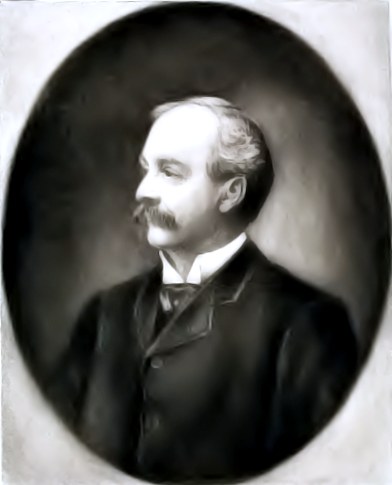
\includegraphics[scale=0.75]{../white/WCCraneWhite.png}
	\caption {WARREN CODY CRANE}
\end{figure}

\begin{figure}[htp]
	\centering
	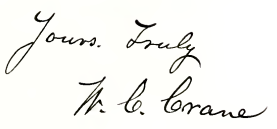
\includegraphics[scale=0.75]{../white/WCCraneSigWhite.png}
	\caption {WARREN CODY CRANE'S SIGNATURE}
\end{figure}



WARREN CADY CRANE (Austin, Aaron, Ebenezer,5 John,' Ebenezer,' John,' Henryi), born in West 
Granville, Hampden Co., Mass. ; married Caroline E. Cleveland, 
a native of Winsted, Conn., at that place, Oct. 10, 1865. But 
soon removed from there to Brooklyn, N. Y., and subsequently 
from there to New York City, where he is engaged in the dry 
goods trade and is a successful merchant. Children : 



Ebeuezer,' John,' Ebeuezer,3 John,2 Henryi), born in Hartlaud, Conn. ; married Albert P. Woodruff at Bristol, Sei)t. 15, 
1852, aud settled iu Forestville. Cliildreu : 



Ebeuezer,' Johu,' Ebeuezer,' Joliu,' Henryi), uiarricd .Inlia 
George, aud resided iu ludiauapolis, lud. Cliildreu : 


Ebeuezer,' Johu,' Ebeuezer,' Johu,' Heury'), married at Water- 
bury, Couu., Ettie L. Morris, April 21, 1.S7.S. She was daui>liter 
of William F. aud Elizabeth Morris, aud was boru June H, is57, 
at Oakville, Couu. Mr. Craue is a mechanical eugiueer aud 
resides at Waterbury, Couu. Childreu : 


Daniel,' Daniel,'* Ebeuezer,' Johu,~ Heuryi), boru in Hornells- 
ville, N. Y. ; married at that place, April 30, 1879, Sarah Juhu- 
Mr. Craue was a graduate of Cary Semiuary, Genesee Co., N. 
Y. ; occupation, banker, aud was for many years cashier of 
Crane's Bank, Horuellsville, N. Y., where he resides. Childreu : 

U29-2: Berth!; \}b- """ '2, 1880, at Rochester, N. Y. 

Beujamiu,' Daniel,' Ebeuezer,' Johu,' Heuryi), married Annie 
L. Jones, May 3, 1877, aud settled in Hartford, Conn., hut later 
removed to New Haven, Couu., at which place he made his home 
iu 1895. Children : 


min, ' Daniel,' Ebeuezer,' John,- Henry'), uuirried (ieorge A. 
Baker, Jr., June 1, 1876, and settled iu New York City. Slie 
afterwards married Edward P. Schuyler of New York.' Child : 


James,5Ezra,4Nathauiel,3Theopliilus,- Henry"), born in .Mi.ldk- 
bury, Vt. ; enlisted aud served iu the late war, principally iu the 




Department of Tennessee; married, Feb. 14, 1877, at Helena, 
Mont., .Tnlia I. Payne, a native of New Mexico, born Oct. 9, 
he was postmaster four and one-half years, notary public six 
years. About 1879 he removed to Fort Benton, and in 1894 was 
a prosperous merchant there and also notary public. Children : 




14384:. George Wilber, b. Aug. 16, 1886, at Fort Benton, Mont. 

1439\_5, Julia Ione, b. Jan. 21, 1890, at Fort Benton, Mont. 

1440-6. , b. March 8, 1894, at Fort Benton, Mont. 

Ezra,'* Nathaniel, 3 Theophilus,' Henry'), married Charles Elston, 
and were in 1894 residing in Defiance, Woodson Co., Kan. 

Children : 






James, ' Ezra,"* Nathaniel, 3 Theophilus,' Henryi), was born in 
Ridgeville, now Evanston, 111. ; married . Children : 





James,' Ezra,"" Nathaniel, ' Theophilus,' Henryi), married Delia 
J. Crain [1256], daughter of Frances B. Crain of Farm Hill, 
Pierce Co., Wis., Dec. 24, 1884. Children: 

1450-3. Blain. 

Ezra,' Nathamel,3 Theophilus,' Henryi), married O. D. Angle, 
a native of New York, in Evanston, 111., where they first settled. 
By trade he was a carpenter, but for some years was foreman 
he purchased a farm near Charlotte, Mich., where he resided 
until 1892, when he sold it and returned to Evanston to live. 
Mr. Angle served three years, as a soldier in the late war. 

Children : 



Griffln of Charlotte, Mich. 







Ezra,-* Nathauiel,3 Theophilus,' Heuryi), married, March 4, 
on the western frontier, and in 1887 was in company with his 
brothers William and George engaged in the horse hiisiness at tlie 
West, but of late years has made his home in Kvaiiston, 111., 
where he has been employed in the meat business. Children : 


James, 5 Ezra,' Nathaniel, ' Theophilus,- Henryi), married, April 
4, 1887, Wallace H. Blake of J'vanston, 111., and there they have 
resided. He is in the employ of H. Hoyt \& Co., wholesale 
grocers of Chicago. Children : 



Ezra,4 Nathaniel, 3 Theophilus,' Henryi), married, Nov. 7, IHJSl), 
Amelia C. Lewis, sister to his brother Charles' wife. On leaving 
school he secured a position in McClurg's book-store, but soon 
applied for a situation with the Chicago \& North- Western K. K. 
Co., was accepted, and for many years has been in llie employ of 
that company, now (1895) holding the position of discount clei-k 
in the freight auditor's department. Children : 


man,6 Martin,' Ezra,' Nathaniel, ' Theophilus,- Henry' ). innrricd, 
Jan. 1, 1886, Sarah Jane Wilson. Child: 


Ezra, 4 Nathaniel, 3 Theophilus, ' Henryi), married Nellie J. 
Havens, Jan. 1, 1883, at Ogsdeuburg, N. Y., where they n'sifU- 
and where she was born May 5, 18G6. Mr. Crane ii'Cfivt'd his 
education through the schools of Canton, N. V.. the iilacc of iiis 
nativity, and has been employed as a salesman. Child : 


miah,-"' P'zra,-* Nathaniel,' Theoi)liilus,- Hemyi). niMiii.Ml ;it 
Rensselaer Falls, N. Y., Elmer E. Ilellegas, .Jan. 2(1, 1M>2. He 




was a native of De Kalb, N. Y., born June 30, 1871, and now 
(1894) resides there ; a farmer by occupation. Cliild : 


Simeon, 5 Ezra,' Nathaniel,' Theophilus,' Henryi) , married Cliarles 
Valentine Smitli, editor St. Joseph County Republican. She died 
May 1, 1886. Their residence was Centreville, St. Joseph Co., 
Mich. He died quite suddenly while at the neiohborino- city of 
Grand Rapids, Mich, Feb. 1, 1888. Child: 


William," Aaron, ' Ezra,' Nathauiel,' Theophilus,' Henry'), mar- 
ried, Oct. 29, 1873, Harriet Elizabeth Buckley. Children : 

1466-1. Harry Braker, b. June 2, 1876, at Yonkers, N. Y. ; d. July 


Ezra,4 Nathaniel, 3 Theophilus,' Henry'), married Elmer E. Ide 
at Troy, N. Y., Aug. 6, 1884. Children : 





Aaron, ' Ezra,'* Nathaniel, ' Theophilus,' Henryi), married Charles 

B. Wilson at Troy, N. Y., Oct. 25, 1881. For a time they lived 
in Troy, N. Y., but for some years their residence has been at 
Saratoga Springs, N. Y. Children : 




Aaron, 5 Ezra,'* Nathaniel, ' Theophilus,' Henry*), married Buleah 
Dunham, June, 1893. Child : 

1471'  '1. Laura Elizabeth. 

Aaron, 5 Ezra,' Nathaniel,' Theophilus,' Henry*), married George 

C. Butler at Corinth, N. Y., Oct. 24, 1889. Children: 



Phineas," Robert G.,' Silas,' Henry,' Henry*), married Alice 




Rowland, Dec. 30, 1885, and was residino- in Proctorvillc, :Mo., 
in 1894. Child : 


Phineas,' Robert G.,' Silas, ' Henry,'- Henry'), married (ieorue 
E. Nichols, Sept. 27, 1880, and in 1894 were residinu; in Fartm, 
N. Dak. Children: 





Phineas,' Robert Cx.,4 Silas, ' Henry, ' Hem-yi), married Flora 
Nellis, Dec. 26, 1888, and settled 'in Proctorville, Mo., where 
they were li\\'ing in 1894. Children : 




\chapter{CRANES AS LAWMAKERS AND PUBLIC OFFICIALS}



A list of Cranes are here presented who served in Connecticut 
as Lawmakers and public otiicials. No attempt, however, has 
lieen made to ascertain the names of descendants of the female 
lines who may have rendered equally as worthy service. Those 
who are among the descendants of Henry Crane of Guilford have 
notes referring to the numbers where their names appear in the 
body of the book. Explanatory notes also point to the ancestor 
or progenitor of the other persons whose names appear in the list. 
It was contributed by William Wallace Lee of Meriden, Conn., 
grandson of Clarenda Crane, No. 656, page 98. His family. No. 
663, page 100. Mr. Lee is deeply interested in family history, 
and fully realizing the task of collecting and compiling genealogi- 
cal data, has had the goodness to supply the following, with other 
conti-ibutious, thereby adding greatly to the value of the book. 



While it does not necessarily follow that lecause a man has 
been selected for official position that he is either good or great, 
yet it does prove that to be repeatedly chosen to such positions 
he must have the esteem and confidence of those who know him ; 
and it further follows that to retai-n that confidence and regard 
he must be of good repute before the world. All public officials 
will, in the long run, represent the average virtue and morality 
of those by whose votes they have been chosen to office, whether 
in church, civil, or military life. Hence we are justified in the 
belief that in a community, composed as were the early colonies, 
of men of such sturdy moral and religious convictions, no one of 
loose morals or lax living would be called to officiate in any 
public capacity. So we may, without egotism, I think, justly 
claim that the Cranes mentioned in this article were at least fair 
representatives of morality and intelligence of the early Conntc- 
ticut pioneers. 

The matter contained in this article has been carefully com- 
piled from a thorough search of the ancient colonial records and 
a review of all the lists of legislators in Connecticut from H\\"7 
down to and including the year 1800. While I do not claim that 
it is perfect in every particular, I am certain that the omissions, 
if any, are very few. I have personally gone over the entire list, 
preferring to trust my own labors rather than any one else. 




As my Grandmother Clarenda Crane Sumner died when I was 
a mere child, as did my mother a few years later, I grew up in 
ignorance of my mother's relatives and only learned when past 
tracing out the descendants of John Lee (who came to Boston in 
1634, "to Hartford in 1635, becoming one of the proprietors of 
Farmington, Conn., in 1641), with our allied families of Hart, 
Hubbard, Sedgwick, Hayes, I knew something of the nature of 
the task our kinsman, E. B. Crane, had in store ; and knowing 
also that matter culled from our ancient records have an interest 
and are sometimes a help to those who are engaged in tracing out 
family histories, I, in this manner, offer what I have gathered 
pertaining to the Crane family. 

The settlements that were on the banks of the Connecticut 
River, at Hartford, Windsor, and Wethersfield became, when 
united under one government in 1637, the original Connecticut 
Colony, and maintained its colonial existence until the Declara- 
tion of Independence in 1776. The first settlement at New 
Haven or Quinipiac was made in 1639, and the same year a por- 
tion of the emigrants made settlements in Milford and Guilford. 
These settlements united with the one at Quinipiac and became 
the New Haven Colony, and so continued a separate existence 
until 1664. As these colonies were less than 40 miles apart and 
in a few years many removed from one to the other it was but 
natural that questions would arise of sometimes serious difference, 
and so jealousies and sometimes acrimonious disputes would fol- 
low. The story is too long to tell here in all its details. After 
quite a number of conferences and discussions the two colonies 
were united under one government in 1664, but not without great 
reluctance on the part of many of the more prominent of the 
members of the New Haven Colony ; and this fact explains why 
commissioners were appointed to negotiate with and administer 
the oath of allegiance to the Connecticut Colony. 

From New Haven Colonial Records' Volume I. 

Jasper Crane* was one of the original proprietors ; had the 
fifth seat in the meeting-house in 1646 ; owned land in East 
Meadows ; name appears frequently as serving on committees ; 
arbitrator, etc. ; seems to have been quite prominent in town 
matters. 

Neio Haven Colonial Records' Volume II. 

Jasper seems in this to have become one of the proprietors of 
Totokett or Branford ; was Deputy from that town (or plantation 
as they were sometimes called) to the General Court, May, June, 
August, October, November, March, 1653; April, May, June, 
August, October, January, 1654; October, 1655; March, 1656; 
May, 1657; May, 1659; May, 1660; May, 1661; May, 1662; 
May, 1663; May, 1664; also show that he was Magistrate or 




I IC.V.i: 


<\\v I'l-olll 


i." If-sl. 


', 1701, 


; Com- 


), ICix;, 


> Olll" of 


['oiiiitrv 




Connecticut Colonial Records, Volume I. 

Jasper Crane in 1664 was appointed one of the t'oininissiDncis 
to administer tlie oath of allegiance to all the freemen of New 
Haven Colony after the nnion'with the Coniieetieut Colony. In 
Colony against " De Ruyter," the Dutch Admu-al.' who was then 
cruising in the Sound and threatening the settlements along the 
coast. 

New Haven Colonial Records, Volume II. 

Henry Crane* is enrolled as a freeman in Guilford ii 
appears as a Deputy in the Connecticut Colonial Asscnih 
Killing-worth in 1675, 1678, 1679, 1680, l(;.si, ](;s2, IC.s; 
1702; was Justice of the Peace in l(i98, 1701, 1702, 1703 : 
missioner of the Court 1690, 1691, 1692, 1693, 1694, 1695, 

Benjamin CRANE,t senior, of Wethei'sfield in 16.Si\\ w; 
the petitioners to set out a plantation in the Wapaquasset d 
(in and about what is now known as Woodstock, Coiui.). 

Jonathan Crane J of Windham, Deputy in Colonial Assemhlv 
in 1701, 1702, 1703, 1705, 1707, 1709, 1711, 1713, 1714, 1717, 
1718, 1721, 1722; Ensign in the Train Band. 1695; Lieutenant, 

John Crane of Killingworth, Deputy in Colonial AssemMy, 
1703, 1705, 1706, 1707, f708, 170!), 17i0, 1711 : Caj.tain in the 
militia, 1708; was Captain in the expedition against Canada in 
1711; died while on his return at New York; funei-al t'xpenses 
paid by the Colony; amount, 19 pounds, 11 shillings, 6 pence. 

Henry Crane|| of Durham, I)ei)uty in Colonial Assembly, 
1730, 1731, 1732, 1733, 1734; Justice of the Peace. 172s. I72',i. 
1730, 1731, 1732, 1733, 1734, 1735, 1736, 1739. 17 lo; Captain 

John Crane' of Mansfield, in 174.'> one of tiic petitionei-s for 
the selection of a meeting-house site in that town. 

John Crane** of Killingworth was First Liculrnant in the ex- 
pedition against Canada in 1760; was Captain in 17i'il: Deputy 

Daniel CRANEft of Killingwortli as adniinistiator one >tate of 
Samuel Stevens petitions for leave to sell land 175:i. 



* See page 52, Xo. 1. t Was brotlier of Henry, p 


||See page (i.5. No. :U. t<'i"it"""'J" <'f Henjamin. 

**See page 70, No. 105. tfSee page 74, No. 15:5. 




Zebulon Crane* of Kent asks leave to sell land as executor in 

Stephen Crane and Adonijah Crane, f both of New Milford, 

Captain Samuel Crane, J Representative from Killing-worth, 
May, 1779, October, 1779, May, 1780, October, 1780, October, 

Joel Crane of Southbury, Representative, May, 1813, Octo- 




Darius CRANEff of Ellington, Representative, 1850 ; Senator, 
1853, 20th District. 


The New Haven Colonial Records are in two volumes only. The 



*Great-grandson of Benjamin. fGreat-grandsons of Benjamin. 

JSee page 75, No. 172. Descendant of Jasper. 

IJDescendant of Benjamin. 'Descendant of Benjamin. 

**Descendant of Benjamin. ffDescendant of Benjamin. 

IJSee page 130, No. 1006. Descendant of Benjamin. 

IJIlDescendant of Benjamin. ffDescendant of Benjamin. 



\chapter{THE CRANE GALLEY.}


During the Revolutionary War the Coiuu'cticut Colony, in 
order to iucrease facilities for her coast defence, caused to l)e 
put into service three boats, or galleys as they were called. They 
were named the Shark, which was built at Norwich and com- 
manded by Capt. Stanton, the Whiting by Capt. McCk'ave. and 
the Crane. The latter named in honor, no doul)t, of the family 
who so loyally stood by the Colony. The Crane was commanded 
by Capt. Jehiel Tinker. Each galley was manned with 50 men, 
including officers, the latter consisted of a captain, two lieuten- 
ants, a master, a gunner, a mate, a steward, two sergeants of 
marines, two corporals of marines, a boatswain, a drunnner, a 
fifer, a cook, a carpenter's mate, a surgeon or mate. June 20, 
1776, Capt. Tinker was ordered to proceed to New London. Six 
days later two of the nine-pound cannons at New London wvw 
orders came to take two three-pounders from the old fort there, 
also eight swivel guns soon as could be obtainetl. witli ten 
muskets and such an amount of powder and liall and military 
stores as thought necessary ; that the galley should cruise from 
Stonington to the mouth of the Connecticut River, and as far 
southward as Montauk Point, with precaution and prudence ; 
officers and men to be under the rules of the Continental Fleet 
until further rules should be adopted. July 16, at solicitation of 
Gen. Washington, the galleys Whiting and Crane were ordered 
by the governor and council to proceed to New York to assist in 
the defence there under direction of Gen. Washington. The 
galley Crane was built at East Haddam by Job Wiuslow, at a 
cost of £1013610. 



\chapter{ROLL OF HONOR.}


During the year 1885, while William Wallace Lee, Esq., of 
Merideu, was serving as a Representative in the Connecticut 
Legislature, and occupying his spare moments in examining 
ancient records at the State Library in quest of matters relating 
to his ancestry, much to his surprise he learned that very little 
attention had been given toward accumulating a list of names of 
the men who gave their services in behalf of our National Inde- 
pendence. It seemed to him that the people of Connecticut had 
neglected a very important work ; that a State which sent to 
the front nearly 32,000 men out of a population of about 
170,000, could do no less to show their respect and appreciation 
for their services in that great cause than to prepare a roster of 
their names, so far as possible, that it might serve as a memorial 
to their patriotism and devotion to country. As the discovery 
was made too late for action that year, and having been reelected 
to the Legislature the following session of 1886, he caused a bill 
to be drawn, which he introduced and, after some delay, was, 
chiefly thi'ough his efforts, passed, and a very creditable publica- 
Although the record is not complete, yet it is a most worthy docu- 
ment for the State to issue, and Mr. Lee is to be congratulated 
on his success in accomplishing so much towards perfecting and 
perpetuating the records of the past. And it is through the 
advantages afforded by this publication, and the kindness of Mr. 
Lee in copying the names from that list, that we are able here to 
present the following roll of honor. A few names, however, 
have been added to the list furnished by Mr. Lee of those whg 
went into service from outside the State of Connecticut and were 
descendants of Henry Crane of Guilford or became connected to 
them by marriage. Only those appear in the Roll who were men- 
tioned as having rendered service in their returns to the compiler. 
Some names in the Roll were spelled Crain, but that fact cannot 
change their relationship with the family. The number following 
a name, except where used to indicate date of service, refers to 
the body of the book for further information. 

Henry, served in Indian wars, I. 



\section{REVOLUTIONARY WAR.}
Aaron, descendant of Benjamin of Wethersliekl, served under (icn 

Aarox, descendant of Benjamin of Wethersfleld, Capt. Jonathan .1. Vin- 
son's Co., 177(1. 
Amariah, descendant of Benjamin of Wetberstield, Cant. Ueni 'I'Ihood'n 

Co., 1777 to 17.S0.  

Curtis, descendant of Benjamin of Wetherslield, Capt. Tho.s. Woostcr's 

Co., 1778-1781. 
Curtis, descendant of Benjamin of Wettiersfleld, Capt. Howr .Mden's 

Daniel, descendant of Benjamin of Wetlierstield, Capt. lOxpcrii-iicc 

Danikl, descendant of Benjamin of Wetliersfleld. 
Daniel, descendant of Henry of Guilford, ;i4;!. 
David, descendant of Benjamin of Wethersfield, Caitt. ])ickin,sun"s Co., 

Ebenezer, descendant of Henry of Guilford, 3;]0. 
Elihu, descendant of Henry of Guilford, 20-1. 
Elihu, descendant of Benjamin of Wethersfield, served under Col. 

Elijah, descendant of Benjamin of Wethersfield, Beardsleys Co., 1775; 

Fnller's Co., 177(5. 
Elisha, descendant of Henry of Guilford, oOl. 
Hezekiah, descendant of Benjamin of Wethersfield, Cii|)t. liuswell 

Hezekiah, descendant of Benjamin of Wetherslield. under (ien. (iatcs. 

Hezekiah, Jr., descendant of Benjamin of Wetherslield, Cai)t. Isaac 

Sergeant's Co., 177(1. 
James, descendant of Benjamin of Wethersfield, Cai)t. David Beebe's 

John, descendant of Henry of Guilford, 10;>. 
Jonathan, descendant of Benjamin of Wethersfield, Cai)l. Tlios. Knowl- 

Joseph, descendant of Benjamin of Wetherslield, Capt. John ClRsferV 

Nathaniel, descendant of Henry of (Juilford, I'.x;. 
KuEus, descendant of Benjamin of Wetherslield, ("apt. Kosw.'ll Graiif.s 

KuFUS, descendant of Benjamin of Wetherslield, luider Col. (has. 

Silas, descendant of Henry of Guilford, Col. Samuel Webbs \\lvii., I7>n, 

Simeon, descendant of Henry of (Juilford, !]. 




William, descendant of Benjamin of Wethersfleld, Capt. John Chester's 

William, descendant of Benjamin of Wethersfleld, Capt. Hezekiah 

William, descendant of Benjamin of Wethersfleld. 







George, descendant of Henry of Guilford, under Capt. Jared Strickland. 







\section{WAR OF THE REBELLION.}

2d Lt. Alvin, Co. D, 21st Reg., C. V., enlisted 1862; 1st Lt. July, 1863; 


Charles S., Co. H, 1st Reg., C. V., enlisted 1863; was in Co. F, 8th 





John, Co. C, 14th Reg., C. V., enlisted 1.S65. 






William B., Co. K, 17th Eeg., C. V., enlisted isr,2, iiiusicinii. \\.\\:',2. 
William O., 1:U0. 

Married to, or 1)i;sci:ni>axts hv, fuANKs. 

Belden Greenslett, S87. 
Henry Greenslett, SS8. 
Martin C. Greenslett, S85. 

\end{document}
